%%%%% Set up %%%%%

% Set document style and font size
\documentclass[12pt]{article}\usepackage[]{graphicx}\usepackage[]{color}
%% maxwidth is the original width if it is less than linewidth
%% otherwise use linewidth (to make sure the graphics do not exceed the margin)
\makeatletter
\def\maxwidth{ %
  \ifdim\Gin@nat@width>\linewidth
    \linewidth
  \else
    \Gin@nat@width
  \fi
}
\makeatother

\definecolor{fgcolor}{rgb}{0.345, 0.345, 0.345}
\newcommand{\hlnum}[1]{\textcolor[rgb]{0.686,0.059,0.569}{#1}}%
\newcommand{\hlstr}[1]{\textcolor[rgb]{0.192,0.494,0.8}{#1}}%
\newcommand{\hlcom}[1]{\textcolor[rgb]{0.678,0.584,0.686}{\textit{#1}}}%
\newcommand{\hlopt}[1]{\textcolor[rgb]{0,0,0}{#1}}%
\newcommand{\hlstd}[1]{\textcolor[rgb]{0.345,0.345,0.345}{#1}}%
\newcommand{\hlkwa}[1]{\textcolor[rgb]{0.161,0.373,0.58}{\textbf{#1}}}%
\newcommand{\hlkwb}[1]{\textcolor[rgb]{0.69,0.353,0.396}{#1}}%
\newcommand{\hlkwc}[1]{\textcolor[rgb]{0.333,0.667,0.333}{#1}}%
\newcommand{\hlkwd}[1]{\textcolor[rgb]{0.737,0.353,0.396}{\textbf{#1}}}%
\let\hlipl\hlkwb

\usepackage{framed}
\makeatletter
\newenvironment{kframe}{%
 \def\at@end@of@kframe{}%
 \ifinner\ifhmode%
  \def\at@end@of@kframe{\end{minipage}}%
  \begin{minipage}{\columnwidth}%
 \fi\fi%
 \def\FrameCommand##1{\hskip\@totalleftmargin \hskip-\fboxsep
 \colorbox{shadecolor}{##1}\hskip-\fboxsep
     % There is no \\@totalrightmargin, so:
     \hskip-\linewidth \hskip-\@totalleftmargin \hskip\columnwidth}%
 \MakeFramed {\advance\hsize-\width
   \@totalleftmargin\z@ \linewidth\hsize
   \@setminipage}}%
 {\par\unskip\endMakeFramed%
 \at@end@of@kframe}
\makeatother

\definecolor{shadecolor}{rgb}{.97, .97, .97}
\definecolor{messagecolor}{rgb}{0, 0, 0}
\definecolor{warningcolor}{rgb}{1, 0, 1}
\definecolor{errorcolor}{rgb}{1, 0, 0}
\newenvironment{knitrout}{}{} % an empty environment to be redefined in TeX

\usepackage{alltt}

% File path to resources (style file etc)
\newcommand{\locRepo}{csas-style}

% Style file for DFO Technical Reports
\usepackage{\locRepo/tech-report}

% header-includes from R markdown entry
\usepackage{pdflscape}

%%%%% Variables %%%%%

% New definitions: Title, year, report number, authors
% Protect lower case words (i.e., species names) in \Addlcwords{}, in "TechReport.sty"
\newcommand{\trTitle}{Summary of the annual 2020 sablefish (\emph{Anoplopoma fimbria}) trap survey, October 7 - November 21, 2020}
\newcommand{\trYear}{2021}
\newcommand{\trReportNum}{nnn}
% Optional
\newcommand{\trAuthFootA}{Email: \href{mailto:Lisa.Lacko@dfo-mpo.gc.ca}{\nolinkurl{Lisa.Lacko@dfo-mpo.gc.ca}} \textbar{} telephone: (250) 756-7385}
\newcommand{\trAuthsLong}{Lisa C. Lacko, Schon M. Acheson and Brendan M. Connors}
\newcommand{\trAuthsBack}{Lacko, L.C. and Acheson, S.M. and Connors, B.M.}

% New definition: Address
\newcommand{\trAddy}{Pacific Biological Station\\
Fisheries and Oceans Canada, 3190 Hammond Bay Road\\
Nanaimo, British Columbia, V9T 6N7, Canada\\}

% Abstract
\newcommand{\trAbstract}{This document describes sampling activities and summarizes results from the 2020 British Columbia Sablefish research and assessment survey. The survey was comprised of stratified random sets (StRS) at five depth-stratified areas. A portion of the survey (traditional inlet sets) were removed to shorten the survey in response to the COVID-19 pandemic. Biological sampling for sablefish included collection of length, weight, sex, maturity and age structures. Sablefish were randomly sampled from every third trap on all sets, up to a maximum sample size of 60 sablefish. The tag and release study conducted annually since 1991 was continued in 2020. Sablefish were selected randomly for tag and release from every third trap up to a maximum of 125 fish.

A total of 48,092 sablefish were caught in 2020, of which 3,691 were used for biological samples and 8,200 were tagged and released. Catch per unit effort (CPUE) is an important product from this survey as it is used to infer population trends. In most recent years, survey data from stratified random sets showed increasing trends in CPUE in both mean weight and numbers of fish per trap. At the 2020 StRS sites, the stratified mean survey abundance was 35 kg/trap, down -17\% from 2019 and -13\% from the 2018-2019 average.}

% Resume (i.e., French abstract)
\newcommand{\trResume}{Voici le résumé. Lorem ipsum dolor sit amet, consectetur adipisicing elit, sed do eiusmod tempor incididunt ut labore et dolore magna aliqua. Ut enim ad minim veniam, quis nostrud exercitation ullamco laboris nisi ut aliquip ex ea commodo consequat. Duis aute irure dolor in reprehenderit in voluptate velit esse cillum dolore eu fugiat nulla pariatur. Excepteur sint occaecat cupidatat non proident, sunt in culpa qui officia deserunt mollit anim id est laborum.}

\newcommand{\trISBN}{}

%%%%% Start %%%%%

% Start the document
\IfFileExists{upquote.sty}{\usepackage{upquote}}{}
\begin{document}

%%%% Front matter %%%%%

% Add the first few pages
\frontmatter

%%%%% Drafts %%%%%

%\linenumbers  % Line numbers
%\onehalfspacing  % Extra space between lines
\renewcommand{\headrulewidth}{0.5pt}  % Header line
\renewcommand{\footrulewidth}{0.5pt}  % footer line
%\pagestyle{fancy}\fancyhead[c]{Draft: Do not cite or circulate}  % Header text

%%%%% Main document %%%%%
\hypertarget{introduction}{%
\section{Introduction}\label{introduction}}

Sablefish (\emph{Anoplopoma fimbria}) are a commercially valuable species that are harvested in British Columbia (BC) using trap, longline and trawl gear as part of the integrated management plan for the groundfish fishery. For the past ten years (2011 to 2020), BC fishermen have landed an average of 2,113 metric tons of sablefish annually. The majority of sablefish in 2020 were captured by longline trap gear (55\%) and longline hook gear (40\%). Commercial harvest of sablefish typically occurs at depths up to 985 fathoms, along the steep-walled slopes off the west coast of Haida Gwaii (formerly Queen Charlotte Islands), in the complex troughs of Queen Charlotte Sound, and in the steep canyons and ridges off the west coast of Vancouver Island.

Fishery-independent research and assessment surveys for sablefish have been conducted in BC coastal waters since 1988. Survey procedures have evolved over time, but each year they have consisted of fishing sets using trap gear at randomly selected and/or index sites. These surveys are used to obtain catch rate data, gather biological samples, capture oceanographic measurements and collect tag release and recapture data. This information is used as the key contemporary index of abundance for assessing the biological status of the sablefish stock, and to condition an operating model that serves as the biological basis of the coastal Management Strategy Evaluation (DFO \protect\hyperlink{ref-DFO2020}{2020}).

The design of the sablefish survey has remained consistent since 2011, and has been comprised of stratified random sampling (StRS) for sites along BC's continental shelf and the continuation of sampling at standardized index sites at four mainland inlets. Due to the COVID-19 pandemic, the 2020 survey was shortened and the inlet sites were not surveyed. In addition, a single science crew were contracted from Archipelago Marine Research (AMR) for the duration of the trip. For details about past survey designs, see the historic overview provided by (Wyeth and Kronlund \protect\hyperlink{ref-Wyeth2003}{2003}) and (Wyeth et al. \protect\hyperlink{ref-Wyeth2004b}{2004}\protect\hyperlink{ref-Wyeth2004b}{a}). For details on specific surveys conducted from 1988 through 1993 see (Smith et al. \protect\hyperlink{ref-Smith1996}{1996}); for surveys in 1994 and 1995 see (Downes et al. \protect\hyperlink{ref-Downes1997}{1997}); for surveys from 1996 to 2000 see (Wyeth and Kronlund \protect\hyperlink{ref-Wyeth2003}{2003}). For the 2001 through 2006 surveys see (Wyeth and Kronlund \protect\hyperlink{ref-Wyeth2003}{2003}), (Wyeth et al. \protect\hyperlink{ref-Wyeth2004a}{2004}\protect\hyperlink{ref-Wyeth2004a}{b}), (Wyeth et al. \protect\hyperlink{ref-Wyeth2004b}{2004}\protect\hyperlink{ref-Wyeth2004b}{a}) and (Wyeth et al. \protect\hyperlink{ref-Wyeth2006}{2006}), respectively. Surveys in 2018 and 2019 are found in (Lacko et al. \protect\hyperlink{ref-Lacko2020}{2020}).

In this technical report we describe survey operations and summarize data collected on the 2020 chartered survey aboard the F/V Pacific Viking. Tables and figures referred to in the main text are numbered sequentially. Tables and figures in the appendices are labelled with a letter code. \clearpage

\hypertarget{methods}{%
\section{Methods}\label{methods}}

\hypertarget{survey-design}{%
\subsection{SURVEY DESIGN}\label{survey-design}}

Methodology for the 2020 sablefish research and assessment surveys employed a stratified random sampling (StRS) design. The survey protocol required the StRS component to be completed from the southern end of Vancouver Island to the north coast of Haida Gwaii. The survey design was modified in 2020 in response to the COVID-19 pandemic. The length of the trip was reduced by removing the traditional inlet component of the survey.

\hypertarget{stratified-random-sampling-survey-design-component}{%
\subsubsection{STRATIFIED RANDOM SAMPLING SURVEY DESIGN COMPONENT}\label{stratified-random-sampling-survey-design-component}}

Since 2011, the StRS design has been conducted in all offshore survey areas. The StRS design began in 2003 with the purpose of distributing tag releases at random, collecting biological samples and developing a catch-rate based index of abundance (Wyeth and Kronlund \protect\hyperlink{ref-Wyeth2003}{2003}). It also provided an alternative design to the historic traditional offshore component of the survey (1990 to 2010) which occured at fixed locations.

Under the StRS design the offshore survey area is partitioned into five spatial strata (S\textsubscript{1} to S\textsubscript{5}) and three depth strata (RD\textsubscript{1} to RD\textsubscript{3}) for a total of 15 (Figure~\ref{fig:figure1}). The five spatial strata are S\textsubscript{1} (South West Coast Vancouver Island or SWCVI), S\textsubscript{2} (North West Coast Vancouver Island or NWCVI), S\textsubscript{3} (Queen Charlotte Sound or QCS), S\textsubscript{4} (South West Coast of Haida Gwaii or SWCHG), and S\textsubscript{5} (North West Coast of Haida Gwaii or NWCHG). The three targeted depth ranges are 100-250 fathoms (RD\textsubscript{1}), 250-450 fathoms (RD\textsubscript{2}), and 450-750 fathoms(RD\textsubscript{3}). The area within each of the 15 strata are sectioned into 2 km x 2 km grid cells or `fishing blocks' from which set locations are randomly chosen.

From 2003 through 2005, five grid cells were randomly selected in each spatial-depth stratum. From 2006 through 2010, the number was increased to six. An analysis was completed for the 2011 survey to optimize the allocation of the blocks to strata for the 2011 and 2012 survey. However, in order to lower survey costs, the number of blocks were further reduced for the 2013 survey, from a total of 110 to 91 offshore blocks while maintaining the same relative allocation of blocks to strata. This total number of blocks has been in place on all subsequent surveys (Table~\ref{tab:table1}), including 2020 (Figure~\ref{fig:figure2}).

\hypertarget{vessels}{%
\subsection{VESSELS}\label{vessels}}

The 2020 survey of 87 sets was chartered aboard the 25.34 meter F/V Pacific Viking (Figure~\ref{fig:figure3}), skippered by Albert (Deacon) Melnychuk between Oct 7 - Nov 21 , 2020 (Appendix~\ref{app:first-appendix}). Information about the vessel can be found at \href{http://marinetraffic.com}{\underline{http://marinetraffic.com}}.

\hypertarget{fishing-gear}{%
\subsection{FISHING GEAR}\label{fishing-gear}}

The longline trap gear consisted of a groundline resting on the ocean floor with 25 baited traps attached to beckets at 150 foot intervals along its length and 90 pound anchors at each end (Figure~\ref{fig:figure4}, b). A flagpole was required for at least one end of the set to improve visibility for retrieval. The traps were steel frame with a bottom hoop diameter of 54 inches and covered with an North American \#84 black braided nylon web of 2.75 inch mesh (Figure~\ref{fig:figure4}, a). The tunnels were made of green braided, knotless, 1.25 inch mesh. The traps did not include escape rings; but instead a `rot panel' of \# 21 cotton located above the middle ring.

Standard bait bags (6 by 12 inches) made of 1/8 inch web with a nylon drawstring and \#7 stainless trolling snaps were included with the traps.

\hypertarget{fishing-operations}{%
\subsection{FISHING OPERATIONS}\label{fishing-operations}}

During normal survey fishing operations gear was deployed on alternate days. Prior to deployment, the Fishing Master inspected the block to determine fishability and if it was within the targeted depth range. The goal was to have as much gear as possible within the block boundaries. If unfishable, the survey protocol requires that an alternate block is to be chosen to the east, west, north, and south, respectively. If none of those blocks meet the criteria, an alternate block of the same area and depth strata was randomly chosen. In 2020, the choice of alternate blocks were limited to a pre-selected list prepared by DFO in advance of the survey. Additionally, the crew size was reduced to three and all data collected during fishing operations were recorded on paper forms, rather than electronically.

Two science staff recorded information associated with the deployment of the gear. One science member was positioned in the wheelhouse and recorded set details on the bridge log data form. The start and end geo-referenced positions of each set were entered at the time when the first and last traps were set over the stern. Depths were recorded at one-minute intervals between the first and last anchors being set. Later, the duration of the set was calculated as the time elapsed between the first anchor being set over the stern and the first anchor hauled aboard (Appendix~\ref{app:second-appendix}, Figure B.1).

A set log was filled out on the deck by the science recorder who had maximum visibility of the crew setting the traps over the stern rail. The set log included the time and identity of the first and last buoys, anchor time, a tally of beckets and traps, as well as the unique identifying numbers of sensors deployed (Appendix~\ref{app:second-appendix}, Figure B. 2)

\hypertarget{stratified-random-component-strs}{%
\subsubsection{Stratified Random Component (StRS)}\label{stratified-random-component-strs}}

Sets in StRS blocks had a targeted soak time of 24 hours. Fishing sets were designated useable if hauled between 22 and 26 hours. Traps were baited with 10 pounds of loose offshore Pacific Hake (\emph{Merluccius productus}) and 2 pounds of bagged squid.

\hypertarget{catch-processing}{%
\subsection{CATCH PROCESSING}\label{catch-processing}}

Haulback speed allowed the science crew to accurately record catch. One science and one crew member were positioned on deck at the haul card station; the science staff recorded the catch and the crew member managed the movement of baskets. As the groundline was hauled, each becket and trap were entered in the charter catch log form (Appendix~\ref{app:second-appendix}, Figure B.3). Crew members alerted the recorder about any damage to a trap (i.e.~holes) which was then recorded.

Catch by species from each trap was sorted into baskets by the crew. Baskets were then weighed to the nearest 0.2 kg on a motion compensating scale and given a basket use code of D, A, T, L, SD or F. Code D designated fish species as discards or commercial catch; code A allocated sablefish for age samples; code T allocated sablefish to be tagged and released; code L allocated fish for length samples; code SD identified sublegal sablefish discards; code F represented fish frames with amphipod or hagfish damage (Appendix~\ref{app:second-appendix}, Figure B.3). The next day, the entries on charter catch log form were transposed to tabular format on the charter catch log entry form (Appendix~\ref{app:second-appendix}, Figure B.4).

\hypertarget{sablefish-allocation-details}{%
\subsubsection{Sablefish Allocation Details}\label{sablefish-allocation-details}}

Prior to 2018, sablefish were tagged from 1/3 of the traps on StRS sets and 1/2 of the traps on the inlet sets. Due to high catch numbers, the survey protocol was revised in 2018 to designate \textasciitilde125 sablefish to be tagged (T) from 1/3 of the traps on all sets. When catches were high, traps targeted for tagging were spread throughout the string to avoid tagging the first 125 fish. A biological sample was collected from the coded ``A'' traps with the goal of selecting 50 to 60 fish. If CPUE was high, the new survey protocol of 2018 designated a minimal of two traps to be used for samples. If both traps contained more than 60 sablefish, a random process was used to select \textasciitilde60 specimens.

The remaining traps were allocated to the discard category and sorted by size into either legal (D) or sublegal (SD) discards. The SD (sublegal discards) code was added during the 2017 survey to account for the large numbers of juvenile sablefish and facilitate their quick return to the ocean. Legal discards (D) of sablefish were kept by the vessel and processed as commercial catch.

\hypertarget{biological-sampling-lwsmo}{%
\subsection{BIOLOGICAL SAMPLING (LWSMO)}\label{biological-sampling-lwsmo}}

Biological samples were collected from sablefish and rougheye/blackspotted rockfish (\emph{Sebastes aleutianus/Sebastes melanostictus}) specimens. Measurements were recorded for fork length (L), body weight (W), sex (S) and maturity level (M) (Appendix~\ref{app:second-appendix}, Figure B.5). Sagittal otoliths (O) were collected and stored for potential ageing by the sclerochronology laboratory. In addition, tissue for DNA was collected from the rougheye/blackspotted rockfish complex for later species determination. Since this complex of two distinct species (Orr and Wildes \protect\hyperlink{ref-Orr2008}{2008}) have similar appearances with slight variations in colour markings and dorsal fin lengths, the sampler visually identifed each specimen as either a rougheye, a blackspotted or a hybrid species. All rockfish and legal-sized sablefish (fork length \textgreater{} 55 cm) that were sacrificed for biological samples were dressed, frozen, and landed as commercial catch.

\hypertarget{sablefish-tagging}{%
\subsection{SABLEFISH TAGGING}\label{sablefish-tagging}}

Fish destined to be tagged were transferred from the sorting area to a tagging tank. A vessel crew member was positioned to retrieve sablefish from the tank and provide assistance with fish handling. A scientist stood at the sample station and tagged fish with a Mark II Long Tagging gun loaded with Floy FD-94 T-bar anchor tags. The tag was inserted on the left side of the fish, 1 cm below and 2-3 cm behind the anterior insertion of the first dorsal fin. Fork length (mm) measurements were taken. Before release, any sampling errors, injuries or damage to the fish were recorded on the tagging form by a second scientist. Tag checks were performed systematically to ensure tag numbers on the data form matched those on the fish specimen (Appendix~\ref{app:second-appendix}, Figure B.6).

\hypertarget{sablefish-tag-recovery}{%
\subsection{SABLEFISH TAG RECOVERY}\label{sablefish-tag-recovery}}

Any previously tagged fish brought aboard may have been treated in one of two ways. First, sablefish with Canadian tags were re-released with a new tag and the previous tag was removed. In addition, any wounds from the old tag were recorded. Second, sablefish with a foreign agency tag or sablefish that had sustained numerous injuries were retained for biological sampling. For these specimens, the tag and otoliths were stored in a bar-coded vial that was later scanned into the GFBioField Tag Recovery Entry form by DFO staff (Olsen \protect\hyperlink{ref-Olsen2010}{2010}). Foreign tags were returned to their country of origin.

During survey years 1992 through 1997 and 2004, previously tagged sablefish were re-released with the same tag. New tagging protocols of replacing the tag began in 2005.

\hypertarget{oceanographic-sensor-data-collection}{%
\subsection{OCEANOGRAPHIC SENSOR DATA COLLECTION}\label{oceanographic-sensor-data-collection}}

A Sea-bird Bird SBE 39 temperature and pressure logger was placed in a protective plastic pipe and attached to the middle trap on the string of gear. Data was successfully collected from 87 sets in 2020 (Appendix~\ref{app:third-appendix}). A SBE 39 was also placed in the tagging tank on hauling days to record water temperature. Data from the SBE temperature and pressure loggers were processed at sea after the set was complete.

\hypertarget{electronic-monitoring-video-data-collection}{%
\subsection{ELECTRONIC MONITORING VIDEO DATA COLLECTION}\label{electronic-monitoring-video-data-collection}}

During haulback, the electronic monitoring (EM) system cameras were activated by the hydraulic sensor. Three standard analog cameras were positioned at optimal viewing angles to record survey activities. Two cameras were stationed along the mast to record the catch as it was processed at the hopper. A third camera was stationed on the side of the wheelhouse to record the traps as they were brought over the rail. The video data from each set was reviewed by science staff the following day to provide quality control on catch data.

\clearpage

\hypertarget{results-and-discussion}{%
\section{Results and Discussion}\label{results-and-discussion}}

\hypertarget{fishing}{%
\subsection{FISHING}\label{fishing}}

The 2020 survey was 46 days long and divided into two legs of 16 and 29 days, with a single day between in Port Hardy. Several weeks of inclement weather contributed to a longer second leg. In total, 27 fishing days were recorded.

Of the 91 original blocks for the StRS portion of the survey, ten were replaced at-sea and four blocks were rejected, for a total of 87 blocks successfully fished (Table~\ref{tab:table1}). Of the ten replacements, one was revoked after on-ground inspection, three were located within unfishable habitat, four had failed to meet depth strata requirements, one was located in a conservation area and one was for an unknown reason (the track-line was in the neighboring block).

\hypertarget{catch-per-unit-effort-cpue}{%
\subsection{CATCH PER UNIT EFFORT (CPUE)}\label{catch-per-unit-effort-cpue}}

The sablefish survey of 2020 have documented recent changes in the sablefish population structure.

\hypertarget{stratified-random-set-cpue}{%
\subsubsection{Stratified Random Set CPUE}\label{stratified-random-set-cpue}}

Catch per unit effort (CPUE), as indexed by kilograms of sablefish per trap, decreased in 2020 across the mid depth strata (RD\textsubscript{2}); and remained steady in the shallow (RD\textsubscript{1}) and deep (RD\textsubscript{3}) depth strata (Figure~\ref{fig:figure5}). Comparison across spatial and depth strata indicate declining CPUE (kg/trap) in areas S\textsubscript{2} to S\textsubscript{5}, but increasing in the most southern area S\textsubscript{1} (Figure~\ref{fig:figure6}). The CPUE (\#fish/trap) across all strata declined remarkably with the exception of the northern strata S\textsubscript{5} (Figure~\ref{fig:figure7}). The mean weight is similar or slightly decreasing compared to 2019 (Figure~\ref{fig:figure8}). The stratified mean survey abundance in 2020 was 35 kg/trap, down -17\% from 2019 and -13\% from the 2018-2019 average (Figure~\ref{fig:figure9}).

\hypertarget{catch-composition}{%
\subsection{CATCH COMPOSITION}\label{catch-composition}}

A total of forty-two taxonomic groups were represented in the catches in StRS sets in 2020 (Table~\ref{tab:table2}). These included ten roundfish species, seven rockfish species, four flatfish species and twenty-one invertebrate species. Other than sablefish, the most common species, by weight, were Pacific halibut (\emph{Hippoglossus stenolepis}), lingcod (\emph{Ophiodon elongatus}), spiny dogfish (\emph{Squalus acanthias}), yelloweye rockfish (\emph{Sebastes ruberrimus}) and redbanded rockfish (\emph{Sebastes babcocki}).

\hypertarget{sablefish-sampling}{%
\subsection{SABLEFISH SAMPLING}\label{sablefish-sampling}}

A detailed breakdown of the fate of the catch in each trap for the 2020 survey is listed in Appendix~\ref{app:fourth-appendix}.

During the 2020 StRS, a total of 48,092 sablefish were caught. Of that total, 8,277 were tagged and released and 3,691 were retained for biological sampling. Of the tagged fish, 77 were previously tagged fish that were re-released with a new tag. One previously tagged fish was retained for sampling (Appendix~\ref{app:fifth-appendix}).

Overall, the StRS sets had a higher proportion of females than males over all spatial strata (Table~\ref{tab:table3}). More females than males were caught in the shallow depth stratum within all spatial strata. In the mid depth stratum, there were more males than females in S\textsubscript{1}, S\textsubscript{2} and S\textsubscript{5}. The deepest depth stratum saw more females in spatial strata S\textsubscript{1}, S\textsubscript{2}, S\textsubscript{3} and S\textsubscript{4}.

Significant differences in length distributions between female and male sablefish are exhibited in the data collected from the StRS portion of the 2003 - 2020 surveys. The mean fork length (\(\bar{x}\)) for females was 65.0 cm and the mean fork length (\(\bar{x}\)) for males was 58.4 cm (Figure~\ref{fig:figure10}).

In 2020, the average mean fork length for the 1,925 females was 60.4 cm and the average mean fork length for the 1,676 males was 54.8 cm. The mean length of both females and males reached their lowest mean size since 2003 (Figure~\ref{fig:figure11}).

On average, female sablefish grow faster and reach a far greater size (Figure~\ref{fig:figure12}a) compared to males (Figure~\ref{fig:figure12}b).

\hypertarget{sablefish-sub-legal-encounters}{%
\subsection{SABLEFISH SUB-LEGAL ENCOUNTERS}\label{sablefish-sub-legal-encounters}}

Distinct distribution patterns became apparent across strata of increasing sub-legal sablefish (\textless55 cm fork length), following highly anomalous warm ocean conditions known as the ``Blob'' and the ``Blob 2.0''. The first marine heat wave (Blob) began in the NE Pacific in late 2013 (Bond et al. \protect\hyperlink{ref-Bond2015}{2015}) and persisted until 2016 (Dorantes-Gilardi and Rivas \protect\hyperlink{ref-DORANTESGILARD2020}{2019}). A similar marine heat wave (Blob 2.0) with warm sea surface temperatures appeared again in the summer of 2019 (Amaya \protect\hyperlink{ref-Amaya2020}{2020}).

More than half of the sub-legal specimens were captured in the southern strata (S\textsubscript{1}) mid-depth waters (RD\textsubscript{2}) in 2014 and shallow waters (RD\textsubscript{1}) in 2015. The sub-legal specimen count was above 50\% in both 2017 and 2018 in the northern strata of S\textsubscript{4} and S\textsubscript{5} mid-depth waters (RD\textsubscript{2}). In 2019, the sub-legal specimens dominated in all StRS survey strata (S\textsubscript{1} to S\textsubscript{5}) mid-depth waters (RD\textsubscript{2}). In 2020, the sub-legal specimen count was over 50\% in S\textsubscript{1}, S\textsubscript{4} and S\textsubscript{5} in the mid-depth waters (RD\textsubscript{2}) (Figure~\ref{fig:figure13}).

\hypertarget{recovered-tagged-sablefish}{%
\subsection{RECOVERED TAGGED SABLEFISH}\label{recovered-tagged-sablefish}}

Of the 77 Canadian tagged fish that were recovered on the survey, the majority (79\%) had travelled no more than 50 kilometers of the release site. Most recoveries (70\%) were recaptured within 5 years at liberty (Table~\ref{tab:table4}). Three fish were recovered a second time and released a third time (Table~\ref{tab:table5}).

\hypertarget{other-fish-sampling}{%
\subsection{OTHER FISH SAMPLING}\label{other-fish-sampling}}

Length, sex, maturity, otoliths and DNA samples were collected for 126 rougheye/blackspotted rockfish samples. The science samplers visually identified 68 as rougheye, 58 as blackspotted and none as hybrid species (Appendix~\ref{app:sixth-appendix}).

\hypertarget{sablefish-ages}{%
\subsection{SABLEFISH AGES}\label{sablefish-ages}}

At the time of this report, sablefish ages were only available prior to 2019. The highest proportion of male ages in StRS sets for 2003 through to 2011 were 3, 5, 5, 6, 8, 8, 8, 10 and 12 years of age, respectively. Another cohort appeared in 2012 through to 2016 as 4, 5, 7, 7 and 8 year olds. A cohort also appeared to arrive in 2017 which was dominated by 3 year olds and in 2018 by 5 year olds (Figure~\ref{fig:figure14}b).

The highest proportion of female ages in the StRS sets for 2003 through to 2010 were 3, 4, 5, 6, 7, 8, 9 and 10 years of age, respectively. Then, another cohort appeared in 2011 through to 2015, showing up as 3, 4, 5, 6 and 7 year olds. In 2016, 2017, and 2018 the highest proportion of female sablefish were ages 3, 4, and 5 (Figure~\ref{fig:figure14}a).

Historic data from all samples lists the oldest female sablefish at 92 years of age, collected in 2003 where as the oldest male sablefish with the age of 96 years old was documented for the year 2018.

\hypertarget{oceanographic-temperatures-and-depths}{%
\subsection{OCEANOGRAPHIC TEMPERATURES AND DEPTHS}\label{oceanographic-temperatures-and-depths}}

Co-plots of average temperatures and average depths by 1-degree latitude intervals from south-west Vancouver Island to northwest Haida Gwaii indicate that 2020 survey data exhibited a general trend of decreasing temperature with depth over latitude. The coldest average temperature per set recorded was 2.6 \(^\circ\)C with an average depth of 1295 m in the latitude zone of 52\(^\circ\) - 53\(^\circ\) (Figure~\ref{fig:figure15}).

SBE 39 recorders have been placed on survey fishing sets since 2006. In the shallow waters, the lowest average temperature of 4.1 \(^\circ\)C was recorded in 2016 (latitude zone 52\(^\circ\) - 53\(^\circ\)); the highest average temperature was 7.4 \(^\circ\)C in 2016 (50\(^\circ\) - 51\(^\circ\)) . In the mid-depth waters, the lowest average temperature was 2.9 \(^\circ\)C in 2019 (52\(^\circ\) - 53\(^\circ\)); the highest average temperature was 6.4 \(^\circ\)C in 2013 (50\(^\circ\) - 51\(^\circ\)). In the deepest waters, the lowest average temperature was 2.2 \(^\circ\)C in 2016 (54\(^\circ\) - 55\(^\circ\)) and the highest average temperature was 4.1\(^\circ\)C in 2016 (48\(^\circ\) - 49\(^\circ\)) (Figure~\ref{fig:figure16}).

\hypertarget{acknowledgements}{%
\subsection{ACKNOWLEDGEMENTS}\label{acknowledgements}}

The stock assessment survey and data report is the result of the collaborative efforts of many individuals. Wild Canadian Sablefish has provided coordination and support of the annual Sablefish survey since 1994. The scientific staff that conducted the 2020 sablefish research charter included Guy Boxall, Dean Gaidica, Talyn Ridgway of Archipelago Marine Research Ltd (AMR). A special thanks to the skipper and crew of the F/V Pacific Viking, whose efforts made the survey successful and safe during the COVID-19 pandemic. In 2020, the crew consisted of Deacon Melnychuk (skipper), Cody Melnychuk,Rick Schneider, David Holomego, Rory Johnson and Bruno Olsen.

\clearpage

\hypertarget{tables}{%
\section{Tables}\label{tables}}



\begin{table}[!h]

\caption{\label{tab:table1}Spatial strata allocation and completed strata counts (blue) for the 2020 sablefish research and assessment survey. ~\\
\hspace*{0.333em}\\}
\fontsize{10}{12}\selectfont
\begin{tabular}[t]{l>{\raggedleft\arraybackslash}p{0.5cm}>{\raggedleft\arraybackslash}p{0.5cm}>{\raggedleft\arraybackslash}p{0.5cm}>{\raggedleft\arraybackslash}p{0.5cm}>{\raggedleft\arraybackslash}p{0.5cm}>{\raggedleft\arraybackslash}p{0.5cm}>{\raggedleft\arraybackslash}p{0.7cm}>{\raggedleft\arraybackslash}p{0.5cm}}
\toprule
\multicolumn{1}{c}{\textbf{ }} & \multicolumn{6}{c}{\textbf{Depth Strata}} & \multicolumn{2}{c}{\textbf{ }} \\
\cmidrule(l{3pt}r{3pt}){2-7}
\textcolor{black}{\textbf{Spatia Strata}} & \textcolor{black}{\textbf{RD1}} & \textcolor{black}{\textbf{RD1 2020}} & \textcolor{black}{\textbf{RD2}} & \textcolor{black}{\textbf{RD2 2020}} & \textcolor{black}{\textbf{RD3}} & \textcolor{black}{\textbf{RD3 2020}} & \textcolor{black}{\textbf{Total}} & \textcolor{black}{\textbf{Total 2020}}\\
\midrule
S1 (South West Coast Vancouver Island or SWCVI) & 6 & \textcolor{blue}{6} & 8 & \textcolor{blue}{8} & 5 & \textcolor{blue}{5} & 19 & \textcolor{blue}{19}\\
S2 (North West Coast Vancouver Island or NWCVI) & 6 & \textcolor{blue}{6} & 7 & \textcolor{blue}{7} & 5 & \textcolor{blue}{5} & 18 & \textcolor{blue}{18}\\
S3 (Queen Charlotte Sound or QCS) & 8 & \textcolor{blue}{7} & 6 & \textcolor{blue}{6} & 5 & \textcolor{blue}{4} & 19 & \textcolor{blue}{17}\\
S4 (South West Coast Haida Gwaii or SWCHG) & 6 & \textcolor{blue}{4} & 6 & \textcolor{blue}{6} & 5 & \textcolor{blue}{5} & 17 & \textcolor{blue}{15}\\
S5 (North West Coast Haida Gwaii or NWCHG) & 6 & \textcolor{blue}{6} & 7 & \textcolor{blue}{7} & 5 & \textcolor{blue}{5} & 18 & \textcolor{blue}{18}\\
\midrule
\textbf{Total} & \textbf{32} & \textbf{\textcolor{blue}{29}} & \textbf{34} & \textbf{\textcolor{blue}{34}} & \textbf{25} & \textbf{\textcolor{blue}{24}} & \textbf{91} & \textbf{\textcolor{blue}{87}}\\
\bottomrule
\end{tabular}
\end{table}
\clearpage



\begin{table}[!h]

\caption{\label{tab:table2}Summary of species captured during the 2020 survey StRS sets conducted by the Pacific Viking. No value in the weight column indicates that the catch was not weighed. No value in weight and count of 1 indicates trace weights of less than 1 kg recorded. ~\\
\hspace*{0.333em}\\}
\fontsize{8}{10}\selectfont
\begin{tabular}[t]{lllrr}
\toprule
\textbf{Category} & \textbf{Common Name} & \textbf{Scientific Name} & \textbf{Count} & \textbf{Weight(kg)}\\
\midrule
Roundfish Species & Sablefish & ANOPLOPOMA FIMBRIA &  & 92169\\
 & Lingcod & OPHIODON ELONGATUS &  & 1522\\
 & Spiny dogfish & SQUALUS ACANTHIAS &  & 1122\\
 & Pectoral rattail & ALBATROSSIA PECTORALIS &  & 219\\
 & Pacific grenadier & CORYPHAENOIDES ACROLEPIS &  & 201\\
 & Pacific cod & GADUS MACROCEPHALUS &  & 6\\
 & Pacific flatnose & ANTIMORA MICROLEPIS &  & 2\\
 & Walleye pollock & THERAGRA CHALCOGRAMMA &  & 1\\
 & Pink snailfish & PARALIPARIS ROSACEUS &  & 1\\
 & Pacific viperfish & CHAULIODUS MACOUNI & 1 & \\
\midrule
Rockfish Species & Yelloweye rockfish & SEBASTES RUBERRIMUS &  & 303\\
 & Redbanded rockfish & SEBASTES BABCOCKI &  & 288\\
 & Rougheye/blackspotted rockfish complex & SEBASTES ALEUTIANUS &  & 222\\
 & Shortraker rockfish & SEBASTES BOREALIS &  & 65\\
 & Shortspine thornyhead & SEBASTOLOBUS ALASCANUS &  & 55\\
 & Rosethorn rockfish & SEBASTES HELVOMACULATUS &  & 4\\
 & Longspine thornyhead & SEBASTOLOBUS ALTIVELIS & 2 & \\
\midrule
Flatfish Species & Pacific halibut & HIPPOGLOSSUS STENOLEPIS &  & 1554\\
 & Arrowtooth flounder & ATHERESTHES STOMIAS &  & 287\\
 & Dover sole & MICROSTOMUS PACIFICUS &  & 11\\
 & Petrale sole & EOPSETTA JORDANI &  & 2\\
\midrule
Invertebrate Species & Grooved Tanner Crab & CHIONOECETES TANNERI &  & 117\\
 & Brown box crab & LOPHOLITHODES FORAMINATUS &  & 6\\
 & Oregontriton & FUSITRITON OREGONENSIS &  & 6\\
 &  & ALLOCENTROTUS FRAGILIS &  & 3\\
 &  & PARALOMIS MULTISPINA &  & 3\\
 & Red Queen Crab & LITHODES COUESI &  & 3\\
 & Jellyfish & SCYPHOZOA &  & 2\\
 & Octopus & OCTOPUS &  & 2\\
 & Fish-eating star & STYLASTERIAS FORRERI &  & 1\\
 & Prawn & PANDALUS PLATYCEROS &  & 1\\
 & Sea whip & OSTEOCELLA SEPTENTRIONALIS & 1 & \\
 & Golden king crab & LITHODES AEQUISPINA & 1 & \\
 & Papillose sea cucumber & SYNALLACTES CHALLENGERI & 1 & \\
 & Ophiuroidea & OPHIUROIDEA & 1 & \\
 &  & PYROSOMA & 1 & \\
 &  & SOLASTER & 1 & \\
 &  & TARSASTER ALASCANUS & 1 & \\
 &  & HETEROZONIAS ALTERNATUS & 1 & \\
 &  & MEDIASTER TENELLUS & 1 & \\
 &  & MYXODERMA SACCULATUM & 1 & \\
\bottomrule
\end{tabular}
\end{table}
\clearpage



\begin{table}[!h]

\caption{\label{tab:table3}Summary of sablefish sex ratios and fork length measurements collected during the 2020 stratified random sets by spatial and depth stratum. ~\\
\hspace*{0.333em}\\}
\fontsize{9}{11}\selectfont
\begin{tabular}[t]{llrrrrr}
\toprule
\multicolumn{2}{c}{\textbf{Depth Strata/Locality}} & \multicolumn{2}{c}{\textbf{Proportion}} & \multicolumn{3}{c}{\textbf{Mean Fork Length (mm)}} \\
\cmidrule(l{3pt}r{3pt}){1-2} \cmidrule(l{3pt}r{3pt}){3-4} \cmidrule(l{3pt}r{3pt}){5-7}
\textbf{Spatial} & \textbf{Depth} & \textbf{Males} & \textbf{Females} & \textbf{Males} & \textbf{Females} & \textbf{Tagged}\\
\midrule
S1 & RD1 & 0.34 & 0.66 & 544 & 589 & 563\\
 & RD2 & 0.64 & 0.36 & 516 & 552 & 528\\
 & RD3 & 0.32 & 0.68 & 549 & 612 & 601\\
\midrule
\textbf{} & \textbf{} & \textbf{0.43} & \textbf{0.57} & \textbf{536} & \textbf{584} & \textbf{564}\\
\midrule
S2 & RD1 & 0.28 & 0.72 & 576 & 611 & 595\\
 & RD2 & 0.63 & 0.37 & 547 & 606 & 562\\
 & RD3 & 0.44 & 0.56 & 559 & 639 & 604\\
\midrule
\textbf{} & \textbf{} & \textbf{0.45} & \textbf{0.55} & \textbf{561} & \textbf{619} & \textbf{587}\\
\midrule
S3 & RD1 & 0.33 & 0.67 & 577 & 627 & 607\\
 & RD2 & 0.50 & 0.50 & 548 & 588 & 569\\
 & RD3 & 0.45 & 0.55 & 584 & 662 & 603\\
\midrule
\textbf{} & \textbf{} & \textbf{0.43} & \textbf{0.57} & \textbf{570} & \textbf{626} & \textbf{593}\\
\midrule
S4 & RD1 & 0.21 & 0.79 & 607 & 634 & 623\\
 & RD2 & 0.50 & 0.50 & 529 & 562 & 552\\
 & RD3 & 0.46 & 0.54 & 570 & 646 & 615\\
\midrule
\textbf{} & \textbf{} & \textbf{0.39} & \textbf{0.61} & \textbf{569} & \textbf{614} & \textbf{597}\\
\midrule
S5 & RD1 & 0.21 & 0.79 & 562 & 617 & 587\\
 & RD2 & 0.58 & 0.42 & 541 & 583 & 553\\
 & RD3 & 0.63 & 0.37 & 573 & 627 & 581\\
\midrule
\textbf{} & \textbf{} & \textbf{0.47} & \textbf{0.53} & \textbf{559} & \textbf{609} & \textbf{574}\\
\bottomrule
\end{tabular}
\end{table}
~\\
\hspace*{0.333em}\\


\begin{table}[!h]

\caption{\label{tab:table4}Sablefish tag recovery counts in 2020, by distance from release site and years at liberty. Distances were determined using the great circle distance between the release location and recovery location. ~\\
\hspace*{0.333em}\\}
\fontsize{9}{11}\selectfont
\begin{tabular}[t]{l>{\raggedright\arraybackslash}p{1.1cm}lllllll}
\toprule
\multicolumn{1}{c}{\textbf{ }} & \multicolumn{7}{c}{\textbf{Distance (km) from Release Location}} & \multicolumn{1}{c}{\textbf{ }} \\
\cmidrule(l{3pt}r{3pt}){2-8}
\textbf{Years at Liberty} & \textbf{<10} & \textbf{11-50} & \textbf{51-100} & \textbf{101-250} & \textbf{251-500} & \textbf{501-1000} & \textbf{1000+} & \textbf{Recovery count}\\
\midrule
1 & 13 & 3 & 1 & 0 & 1 & 1 & 0 & 19\\
2-5 & 25 & 3 & 1 & 5 & 0 & 1 & 0 & 35\\
6-10 & 3 & 4 & 0 & 1 & 2 & 0 & 0 & 10\\
11+ & 7 & 3 & 1 & 2 & 0 & 0 & 0 & 13\\
\midrule
Total Counts & 48 & 13 & 3 & 8 & 3 & 2 & 0 & 77\\
\bottomrule
\end{tabular}
\end{table}
\clearpage



\begin{table}[!h]

\caption{\label{tab:table5}Tag history of the events of three previously tagged sablefish recovered on the 2020 survey. Measurement errors (instrumental, environmental or observational) may have caused the shortened lengths. ~\\
\hspace*{0.333em}\\}
\fontsize{9}{11}\selectfont
\begin{tabular}[t]{>{\raggedright\arraybackslash}p{1.7cm}>{\raggedright\arraybackslash}p{1.7cm}>{\raggedright\arraybackslash}p{1.1cm}>{\raggedleft\arraybackslash}p{0.7cm}>{\raggedleft\arraybackslash}p{0.7cm}>{\raggedleft\arraybackslash}p{0.7cm}>{\raggedleft\arraybackslash}p{0.7cm}>{\raggedright\arraybackslash}p{1.3cm}>{\raggedright\arraybackslash}p{3.2cm}>{\raggedleft\arraybackslash}p{0.7cm}}
\toprule
\textbf{Release Tag number} & \textbf{Previous Tag number} & \textbf{Event} & \textbf{Event no.} & \textbf{Event Trip} & \textbf{Event Set} & \textbf{Event year} & \textbf{Date} & \textbf{Fish State} & \textbf{Length (mm)}\\
\midrule
A00550705 &  & RELEASE & 1 & 48110 & 29 & 2002 & 10/15/2002 & LIVE, RE-RELEASED & 595\\
A00545713 & A00550705 & RELEASE & 2 & 80471 & 29 & 2016 & 10/20/2016 & LIVE, RE-RELEASED & 590\\
A00125680 & A00545713 & RELEASE & 3 & 85690 & 32 & 2020 & 10/20/2020 & LIVE, RE-RELEASED & 590\\
\midrule
A00315966 &  & RELEASE & 1 & 77830 & 51 & 2015 & 10/26/2015 & LIVE, RE-RELEASED & 535\\
A00984002 & A00315966 & RELEASE & 2 & 84250 & 62 & 2018 & 11/1/2018 & LIVE, RE-RELEASED & 525\\
A00866014 & A00984002 & RELEASE & 3 & 85690 & 49 & 2020 & 10/25/2020 & LIVE, RE-RELEASED & 544\\
\midrule
A00733036 &  & RELEASE & 1 & 58145 & 33 & 2004 & 10/21/2004 & LIVE, RE-RELEASED & 549\\
A00254854 & A00733036 & RELEASE & 2 & 69067 & 64 & 2009 & 10/28/2009 & LIVE, RE-RELEASED & 575\\
A00493546 & A00254854 & RELEASE & 3 & 85690 & 45 & 2020 & 10/25/2020 & LIVE, RE-RELEASED & 619\\
\bottomrule
\end{tabular}
\end{table}
\clearpage

\hypertarget{figures}{%
\section{Figures}\label{figures}}


\begin{figure}[htb]

{\centering \pdftooltip{\includegraphics[width=410px]{c:/github/surveyreport_2020/figures/figure1}}{Figure \ref{fig:figure1}} 

}

\caption{Location of the boundaries of the five spatial areas (S\textsubscript{1}-S\textsubscript{5}) of the 2020 stratified random survey design. The three depths strata (RD\textsubscript{1}-RD\textsubscript{3}) are colour-coded and nested within each of the five spatial strata.}\label{fig:figure1}
\end{figure}
\clearpage


\begin{figure}[htb]

{\centering \pdftooltip{\includegraphics[width=480px,height=381px]{c:/github/surveyreport_2020/figures/figure2}}{Figure \ref{fig:figure2}} 

}

\caption{Start locations of survey sets (red markers) conducted in 2020 for the stratified random survey areas S\textsubscript{1} through S\textsubscript{5}.}\label{fig:figure2}
\end{figure}
\clearpage


\begin{figure}[htb]

{\centering \pdftooltip{\includegraphics[width=480px,height=480px]{c:/github/surveyreport_2020/figures/figure3}}{Figure \ref{fig:figure3}} 

}

\caption{Image of the F/V Pacific Viking used for the 2020 sablefish research and assessment survey. Photo by Cody Melnychuk.}\label{fig:figure3}
\end{figure}
\clearpage


\begin{figure}[htb]

{\centering \pdftooltip{\includegraphics[width=380px,height=626px]{c:/github/surveyreport_2020/figures/figure4}}{Figure \ref{fig:figure4}} 

}

\caption{Trap elements (A). Trap gear elements consisting of 25 baited traps snapped to beckets along a groundline (B).}\label{fig:figure4}
\end{figure}
\clearpage


\begin{figure}[htb]

{\centering \pdftooltip{\includegraphics[width=400px]{c:/github/surveyreport_2020/figures/figure5}}{Figure \ref{fig:figure5}} 

}

\caption{Sablefish catch per unit effort (CPUE) by depth and year for StRS sets. Dashed lines delineate depth strata (shallow(RD\textsubscript{1}) = 100-450m, mid(RD\textsubscript{2}) = 450-850m, deep(RD\textsubscript{3}) = 850-1400m).}\label{fig:figure5}
\end{figure}
\clearpage


\begin{figure}[htb]

{\centering \pdftooltip{\includegraphics[width=450px,height=576px]{c:/github/surveyreport_2020/figures/figure6}}{Figure \ref{fig:figure6}} 

}

\caption{Average Sablefish catch per unit effort (CPUE; mean +/- 95\% CIs) by survey strata since 2003. Panels run deep to shallow (left to right) and north to south (top to bottom).}\label{fig:figure6}
\end{figure}
\clearpage


\begin{figure}[htb]

{\centering \pdftooltip{\includegraphics[width=450px,height=576px]{c:/github/surveyreport_2020/figures/figure7}}{Figure \ref{fig:figure7}} 

}

\caption{Average number of sablefish per trap (mean +/- 95\% CIs) by StRS survey strata over time. Panels run shallow to deep (left to right) and south to north (top to bottom).}\label{fig:figure7}
\end{figure}
\clearpage


\begin{figure}[htb]

{\centering \pdftooltip{\includegraphics[width=450px,height=576px]{c:/github/surveyreport_2020/figures/figure8}}{Figure \ref{fig:figure8}} 

}

\caption{Average weight of sablefish (mean +/- 95\% CIs) by survey strata over time. Panels run shallow to deep (left to right) and south to north (top to bottom).}\label{fig:figure8}
\end{figure}
\clearpage


\begin{figure}[htb]

{\centering \pdftooltip{\includegraphics[width=450px,height=576px]{c:/github/surveyreport_2020/figures/figure9}}{Figure \ref{fig:figure9}} 

}

\caption{Annual mean weight of sablefish per trap (kg/trap) (A); annual mean number of sablefish per trap (\#fish/trap) (B); annual mean weight of sablefish (kg) (C) by StRS survey strata over time. Horizontal line is median and blue dots are arithmetic mean.}\label{fig:figure9}
\end{figure}
\clearpage


\begin{figure}[htb]

{\centering \pdftooltip{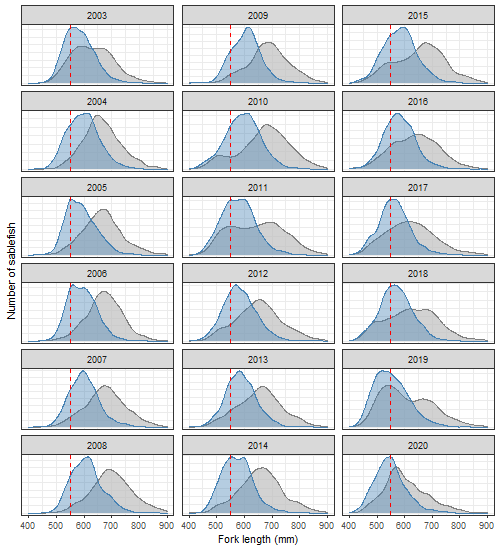
\includegraphics[width=450px,height=354px]{c:/github/surveyreport_2020/figures/figure10}}{Figure \ref{fig:figure10}} 

}

\caption{Length frequencies for female (grey) and male sablefish (steel blue) up to 2020 for all StRS sets. The number of specimens is denoted by the letter n, the mean indicated by the xbar \(\overline{x}\) and the standard deviation is represented by the symbol sigma \(\Sigma\).}\label{fig:figure10}
\end{figure}

\begin{figure}[htb]

{\centering \pdftooltip{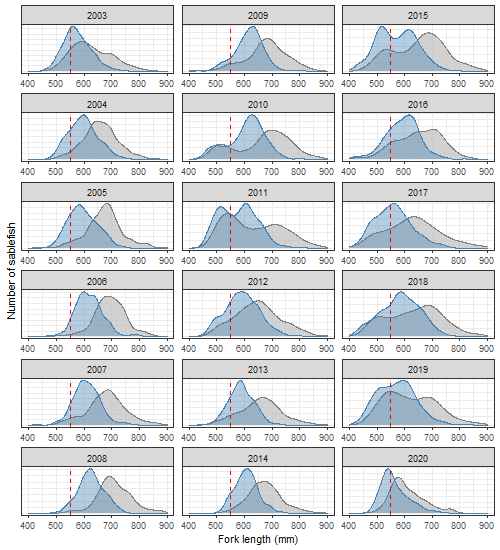
\includegraphics[width=450px,height=276px]{c:/github/surveyreport_2020/figures/figure11}}{Figure \ref{fig:figure11}} 

}

\caption{Average length and ratios of male and female sablefish by year. Counts by sex are labelled on top of the plotted lines.}\label{fig:figure11}
\end{figure}

\begin{figure}[htb]

{\centering \pdftooltip{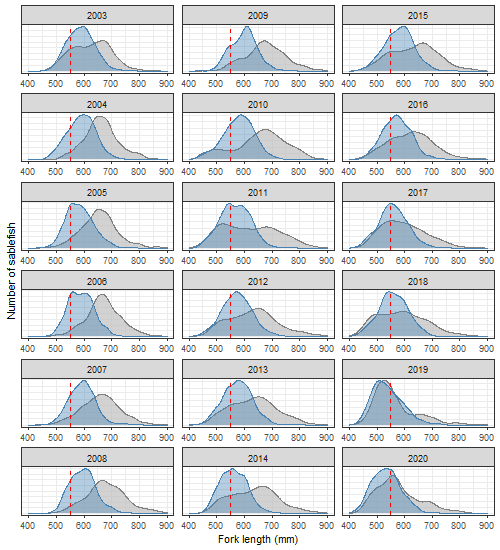
\includegraphics[width=480px,height=282px]{c:/github/surveyreport_2020/figures/figure12}}{Figure \ref{fig:figure12}} 

}

\caption{Sablefish fork length (L in cm) vs weight (W in kg) for females (A) and males (B) for the 2020 survey.}\label{fig:figure12}
\end{figure}

\begin{figure}[htb]

{\centering \pdftooltip{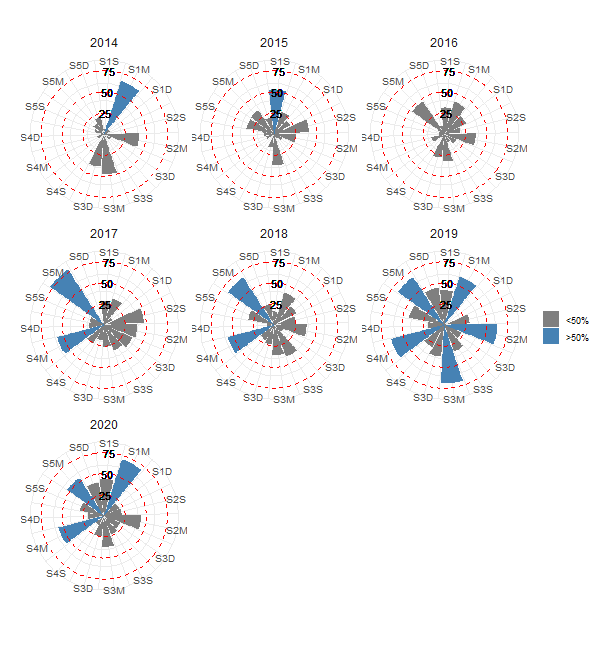
\includegraphics[width=450px,height=500px]{c:/github/surveyreport_2020/figures/figure13}}{Figure \ref{fig:figure13}} 

}

\caption{The percentage of sub-legal sablefish (\textless55 cm fork length) sampled by area (S\textsubscript{1}-S\textsubscript{5}) and depth strata (S=shallow, RD\textsubscript{1}; M=mid, RD\textsubscript{2}; D=deep, RD\textsubscript{3}) over time. Sub-legal specimen count above 50\% sampled shown in blue.}\label{fig:figure13}
\end{figure}
\clearpage


\begin{figure}[htb]

{\centering \pdftooltip{\includegraphics[width=500px,height=577px]{c:/github/surveyreport_2020/figures/figure14}}{Figure \ref{fig:figure14}} 

}

\caption{Bubble plot for female (A) and male (B) sablefish ages by survey year from StRS sets that have been aged. The sizes of the circles are proportional to the number of fish with given ages. Fish age 35 and older are included in one bubble. The total number(n) of fish aged are listed across the top of each panel. The ages with the highest ratios are posted to the right of each bubble.}\label{fig:figure14}
\end{figure}
\clearpage


\begin{figure}[htb]

{\centering \pdftooltip{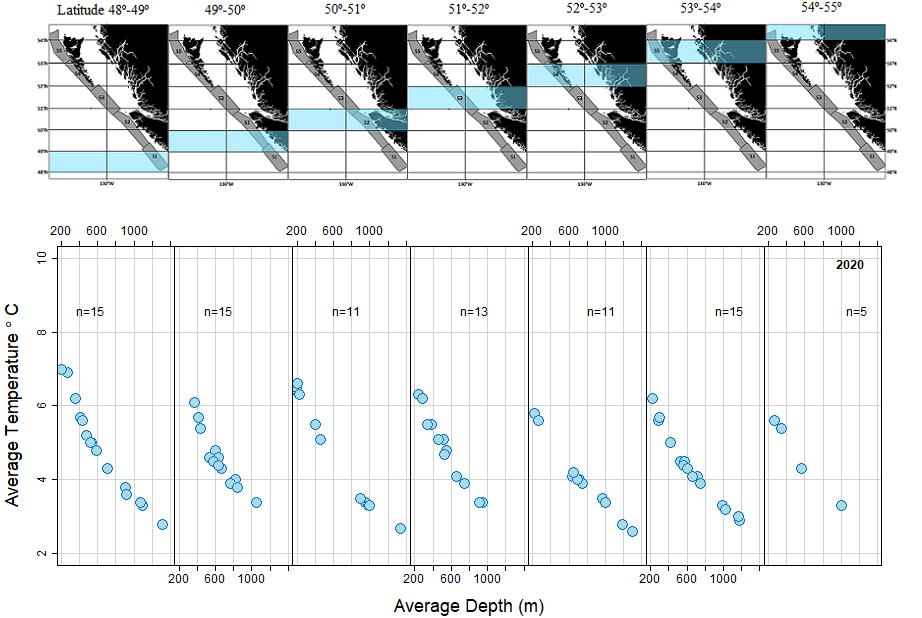
\includegraphics[width=500px,height=335px]{c:/github/surveyreport_2020/figures/figure15}}{Figure \ref{fig:figure15}} 

}

\caption{Coplot of average depth (m) vs average temperature (\(^\circ\)C) for a given 1-degree latitude range (blue bands) for 2020. The number of fishing sets deployed with a SBE 39 recorder are represented by n.}\label{fig:figure15}
\end{figure}
\clearpage


\begin{figure}[htb]

{\centering \pdftooltip{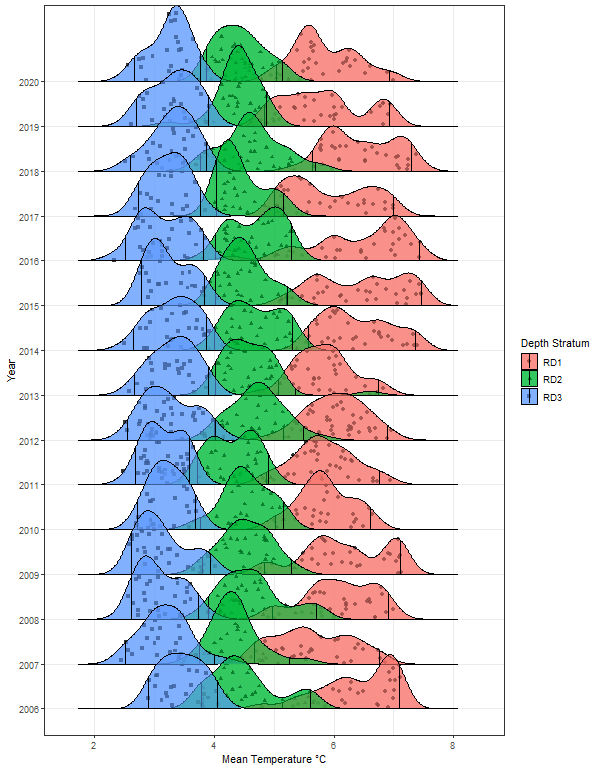
\includegraphics[width=480px,height=616px]{c:/github/surveyreport_2020/figures/figure16}}{Figure \ref{fig:figure16}} 

}

\caption{Vertical density ridgeplots of mean temperatures per year as reported by set from the Sea-bird SBE 39 loggers on traps at three depth intervals, RD\textsubscript{1} = shallow (100-450 m), RD\textsubscript{2} = mid (450-850 m), RD\textsubscript{3} = deep (850-1400 m). Lines indicate the 2.5\% and 97.5\% tails.}\label{fig:figure16}
\end{figure}
\clearpage

\begin{appendices}
\counterwithin{figure}{section}
\counterwithin{table}{section}
\counterwithin{equation}{section}

\clearpage

\section{LIST OF SABLEFISH RESEARCH AND ASSESSMENT SURVEYS.}
\label{app:first-appendix}

\begingroup\fontsize{8}{10}\selectfont
\begin{longtable}{rlllrr}
\toprule
\textbf{Year} & \textbf{Dates} & \textbf{Vessel} & \textbf{Captain} & \textbf{Set Count} & \textbf{GFBIO Id}\\
\midrule
1988 & Oct 28  - Nov 24 & VICIOUS FISHER & VANCE FLETCHER & 16 & 43990\\
1989 & Oct 19  - Nov 18 & LA PORSCHE & SIGURD BRYNJOLFSON & 29 & 43910\\
1990 & Nov  8  - Nov 18 & VIKING STAR & DOUG FARRINGTON & 24 & 43750\\
1991 & Oct  9  - Oct 29 & W. E. RICKER & ALAN FARRINGTON & 32 & 43673\\
1992 & Oct 13  - Nov  4 & W. E. RICKER & RON ROBERTS & 38 & 43670\\
1993 & Oct 19  - Nov 11 & W. E. RICKER & ALAN FARRINGTON & 42 & 43650\\
1994 & Oct 13  - Oct 31 & LA PORSCHE & RICHARD BEAUVAIS & 39 & 43630\\
1994 & Oct 18  - Nov 13 & WESTERN VIKING & RICK JONES & 27 & 43390\\
1995 & Oct  8  - Oct 20 & OCEAN PEARL & ROBERT FRAUMENI & 29 & 43270\\
1995 & Oct 11  - Oct 28 & VICTOR F & MICHAEL DERRY & 34 & 43330\\
1995 & Oct  1  - Oct 31 & VIKING SUNRISE & JASON OLSEN & 40 & 43350\\
1996 & Sep 26  - Oct 10 & OCEAN PEARL & MICHAEL DERRY & 32 & 43039\\
1996 & Sep 30  - Oct 22 & VIKING STAR & OTTO ELVAN & 49 & 43210\\
1996 & May 10  - May 30 & VIKING SUNRISE & ALBERT (DEACON) MELNYCHUK & 42 & 43024\\
1997 & Sep 26  - Oct 21 & OCEAN PEARL & MICHAEL DERRY & 74 & 42699\\
1997 & May 20  - Jun 10 & VIKING SUNRISE & ALBERT (DEACON) MELNYCHUK & 42 & 42760\\
1998 & Sep 22  - Oct 17 & OCEAN PEARL & MICHAEL DERRY & 89 & 41122\\
1999 & Sep 29  - Oct 30 & OCEAN PEARL & MICHAEL DERRY & 109 & 40589\\
2000 & Oct  8  - Nov 14 & PACIFIC VIKING & ALBERT (DEACON) MELNYCHUK & 131 & 40517\\
2001 & Oct  6  - Nov  6 & OCEAN PEARL & MICHAEL DERRY & 134 & 43233\\
2002 & Oct  4  - Nov  7 & PACIFIC VIKING & ALBERT (DEACON) MELNYCHUK & 125 & 48120\\
2002 & Oct  5  - Nov 13 & VIKING SUNRISE & JASON OLSEN & 90 & 48110\\
2003 & Oct 15  - Nov 13 & OCEAN PEARL & MICHAEL DERRY & 94 & 52100\\
2003 & Oct  7  - Nov 10 & VIKING STAR & JIM FARRINGTON & 84 & 52120\\
2004 & Oct  5  - Nov 15 & MILBANKE SOUND & DON QUAST & 95 & 58145\\
2004 & Oct  5  - Nov  3 & OCEAN MARAUDER & ALBERT (DEACON) MELNYCHUK & 84 & 57360\\
2005 & Oct  4  - Nov  2 & PACIFIC VIKING & ALBERT (DEACON) MELNYCHUK & 84 & 60529\\
2005 & Oct  7  - Nov 17 & VIKING SUNRISE & RORY JOHNSON & 88 & 60503\\
2006 & Oct  1  - Nov  1 & PACIFIC VIKING & ALBERT (DEACON) MELNYCHUK & 98 & 62966\\
2006 & Oct  2  - Nov 15 & SENA II & TIM JOYS & 98 & 62666\\
2007 & Oct  7  - Nov 12 & PACIFIC VIKING & ALBERT (DEACON) MELNYCHUK & 99 & 65106\\
2007 & Oct  8  - Nov 12 & VIKING TIDE & JASON OLSEN & 91 & 65107\\
2008 & Sep 29  - Nov 16 & OCEAN PEARL & ROBERT FRAUMENI & 157 & 67007\\
2009 & Oct  8  - Nov 25 & OCEAN PEARL & ROBERT FRAUMENI & 155 & 69067\\
2010 & Oct  9  - Nov 30 & OCEAN PEARL & ROBERT FRAUMENI & 153 & 70787\\
2011 & Oct  9  - Nov 21 & OCEAN PEARL & DARCY NICHOLS & 132 & 72067\\
2012 & Oct  9  - Nov 17 & OCEAN PEARL & DARCY NICHOLS & 135 & 73190\\
2013 & Oct 11  - Nov 17 & PACIFIC VIKING & ALBERT (DEACON) MELNYCHUK & 111 & 74872\\
2014 & Oct  9  - Nov 17 & OCEAN PEARL & DARCY NICHOLS & 111 & 76150\\
2015 & Oct  9  - Nov 20 & PACIFIC VIKING & ALBERT (DEACON) MELNYCHUK & 111 & 77830\\
2016 & Oct  7  - Nov 22 & OCEAN PEARL & DARCY NICHOLS & 111 & 80471\\
2017 & Oct  6  - Nov 21 & PACIFIC VIKING & ALBERT (DEACON) MELNYCHUK & 109 & 82790\\
2018 & Oct  9  - Nov 19 & OCEAN PEARL & DARCY NICHOLS & 111 & 84250\\
2019 & Oct  8  - Nov 25 & PACIFIC VIKING & ALBERT (DEACON) MELNYCHUK & 109 & 85230\\
2020 & Oct  7  - Nov 21 & PACIFIC VIKING & ALBERT (DEACON) MELNYCHUK & 87 & 85690\\
\bottomrule
\end{longtable}
\endgroup{}

\clearpage

\section{DATA FORMS OF THE 2020 SABLEFISH SURVEY.}
\label{app:second-appendix}
\begin{flushleft}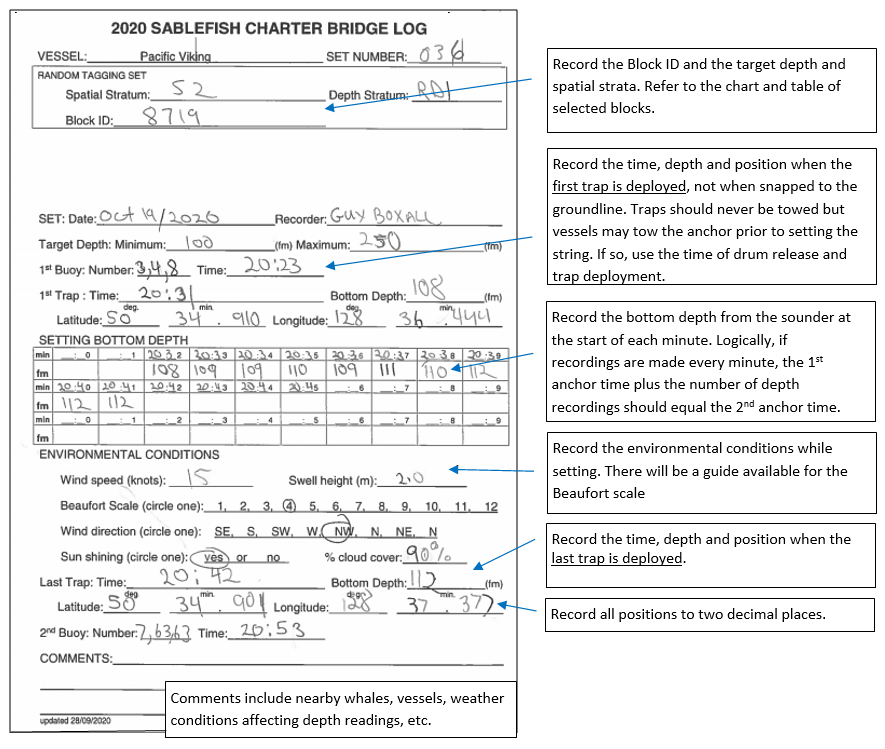
\includegraphics[width=480px,height=406px]{c:/github/surveyreport_2020/figures/AppendixB_BridgeLogIns3} \end{flushleft}

Figure B.1. Example of a completed bridge log data form with directions from the 2020 survey instruction manual.

\clearpage
\begin{flushleft}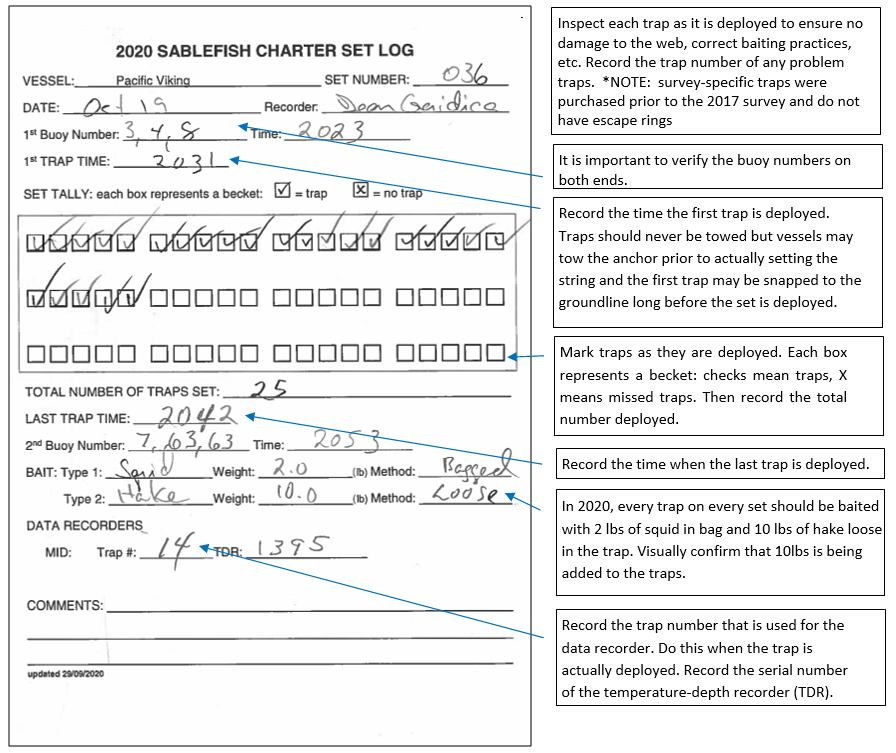
\includegraphics[width=500px,height=420px]{c:/github/surveyreport_2020/figures/AppendixB_SetLogIns3} \end{flushleft}

Figure B.2. Example of a completed set log data form with directions from the 2020 survey instruction manual.

\clearpage
\begin{flushleft}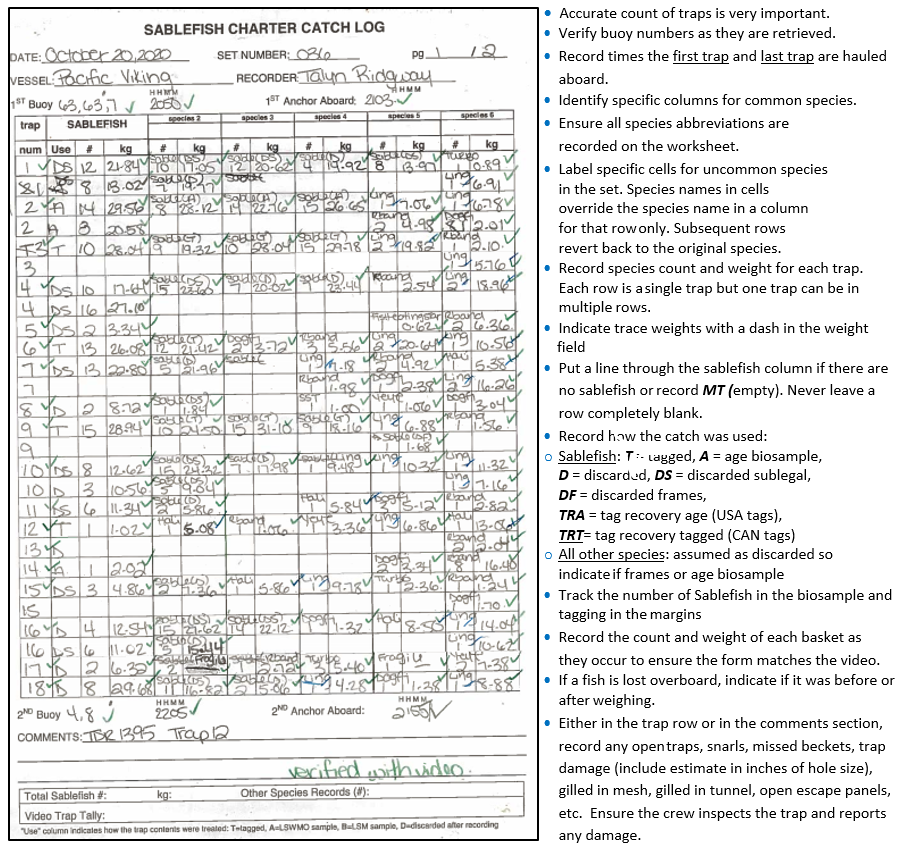
\includegraphics[width=500px,height=476px]{c:/github/surveyreport_2020/figures/AppendixB_CatchLogIns3} \end{flushleft}

Figure B.3. Example of a completed catch log data form with directions from the 2020 survey instruction manual. \clearpage
\begin{flushleft}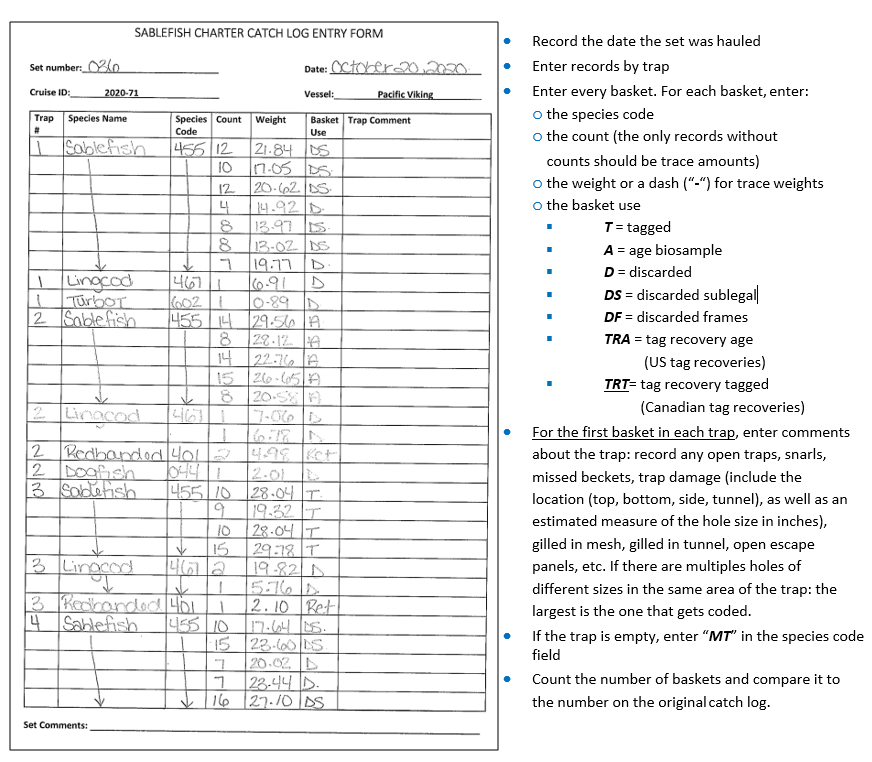
\includegraphics[width=500px,height=426px]{c:/github/surveyreport_2020/figures/AppendixB_CatchLogTabIns3} \end{flushleft}

Figure B.4. Example of a tabular catch log data entry form transposed from the catch log in Figure B.3. Directions from the 2020 survey instruction manual.

\clearpage
\begin{flushleft}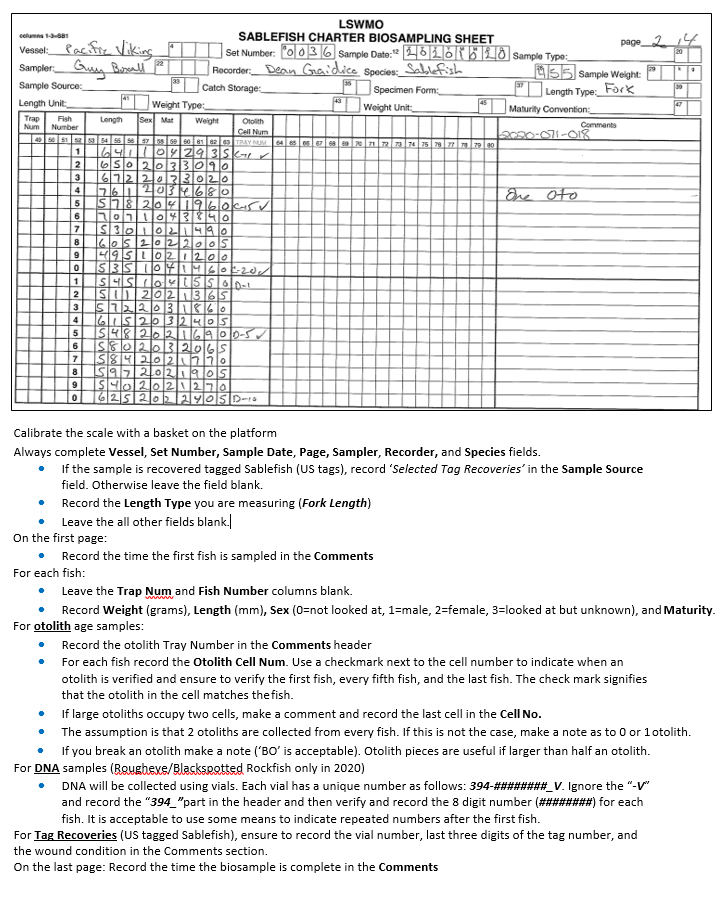
\includegraphics[width=480px,height=588px]{c:/github/surveyreport_2020/figures/AppendixB_LSWMOIns3} \end{flushleft}

Figure B.5. Example of a completed Sablefish biological sampling form and directions from the 2020 survey instruction manual.

\clearpage
\begin{flushleft}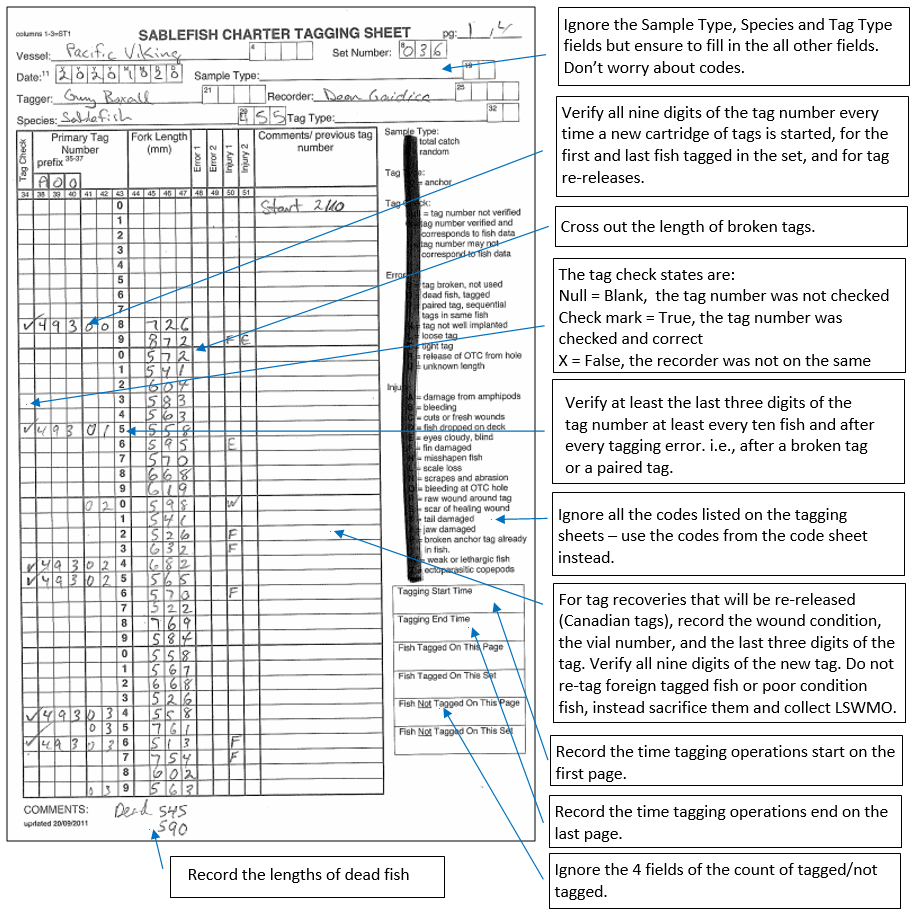
\includegraphics[width=500px,height=501px]{c:/github/surveyreport_2020/figures/AppendixB_TaggingSheetIns3} \end{flushleft}

Figure B.6. Example of a completed tagging form with directions from the 2020 survey instruction manual.

\clearpage

\section{SURVEY SET DETAILS 2020.}
\label{app:third-appendix}

Details of sets completed during the 2020 survey program (F/V Pacific Viking). Sets are listed by stratum/inlet name, set type, depth stratum, start date, end of gear deployment time and duration in minutes. The depth strata for type 3 tagging sets include RD\textsubscript{1} (100-250 fathoms), RD\textsubscript{2} (250-450 fathoms) and RD\textsubscript{3} (450-750 fathoms). The position data includes the major area and start and end latitude and longitude in degrees decimal minutes. The bottom depths (in meters) of the fishing set are shown with the mean bottom depth calculated from recordings at one minute intervals between the start and end of the set. The number of traps fished for each set excludes open traps, while holed or fouled traps have been included. Sets that successfully deployed a Seabird SBE temperature and pressure recorder are indicated with an `x'.
\begin{landscape}\begingroup\fontsize{8}{10}\selectfont
\begin{longtable}{>{\raggedright\arraybackslash}p{0.7cm}>{\raggedleft\arraybackslash}p{0.5cm}>{\raggedright\arraybackslash}p{0.4cm}>{\raggedright\arraybackslash}p{0.7cm}>{\raggedright\arraybackslash}p{0.9cm}>{\raggedright\arraybackslash}p{0.6cm}>{\raggedleft\arraybackslash}p{0.9cm}>{\raggedright\arraybackslash}p{0.5cm}>{\raggedright\arraybackslash}p{1.2cm}>{\raggedright\arraybackslash}p{1.7cm}>{\raggedright\arraybackslash}p{1.2cm}>{\raggedright\arraybackslash}p{1.7cm}>{\raggedleft\arraybackslash}p{0.7cm}>{\raggedleft\arraybackslash}p{0.7cm}>{\raggedleft\arraybackslash}p{0.5cm}>{\raggedleft\arraybackslash}p{0.6cm}>{\raggedright\arraybackslash}p{0.4cm}}
\toprule
\textbf{Spatial Stratum} & \textbf{Set} & \textbf{Type} & \textbf{Depth Stratum} & \textbf{Date} & \textbf{Time} & \textbf{Duration (minutes)} & \textbf{Area} & \textbf{Start Latitude} & \textbf{Start Longitude} & \textbf{End Latitude} & \textbf{End Longitude} & \textbf{Start Depth (m)} & \textbf{End Depth (m)} & \textbf{Mean Depth (m)} & \textbf{Traps Fished} & \textbf{SBE 39}\\
\midrule
\endfirsthead
\multicolumn{17}{@{}l}{continued.}\\
\toprule
\textbf{Spatial Stratum} & \textbf{Set} & \textbf{Type} & \textbf{Depth Stratum} & \textbf{Date} & \textbf{Time} & \textbf{Duration (minutes)} & \textbf{Area} & \textbf{Start Latitude} & \textbf{Start Longitude} & \textbf{End Latitude} & \textbf{End Longitude} & \textbf{Start Depth (m)} & \textbf{End Depth (m)} & \textbf{Mean Depth (m)} & \textbf{Traps Fished} & \textbf{SBE 39}\\
\midrule
\endhead

\endfoot
\bottomrule
\endlastfoot
S1 & 1 & StRS & RD1 & Oct  9 & 08:04 & 1334 & 3C & 48° 7'N & 125° 53'W & 48° 6.4'N & 125° 53.2'W & 405 & 468 & 433 & 25 & x\\
S1 & 2 & StRS & RD3 & Oct  9 & 10:31 & 1398 & 3C & 48° 7.7'N & 126° 7.9'W & 48° 7.5'N & 126° 8.9'W & 904 & 973 & 898 & 25 & x\\
S1 & 3 & StRS & RD3 & Oct  9 & 12:07 & 1421 & 3C & 48° 8.8'N & 126° 13.9'W & 48° 8.8'N & 126° 14.9'W & 1086 & 1092 & 1110 & 25 & x\\
S1 & 4 & StRS & RD2 & Oct  9 & 13:54 & 1429 & 3C & 48° 3.2'N & 126° 10.1'W & 48° 3.8'N & 126° 10.6'W & 477 & 495 & 477 & 25 & x\\
S1 & 5 & StRS & RD1 & Oct  9 & 15:30 & 1479 & 3C & 48° 8.8'N & 126° 10.5'W & 48° 8.8'N & 126° 11.5'W & 336 & 390 & 356 & 25 & x\\
S1 & 6 & StRS & RD3 & Oct  9 & 17:28 & 1534 & 3C & 48° 1.4'N & 126° 21.3'W & 48° 1.5'N & 126° 22.3'W & 982 & 1169 & 1075 & 25 & x\\
S1 & 7 & StRS & RD1 & Oct  9 & 19:37 & 1537 & 3C & 48° 4'N & 126° 9'W & 48° 3.7'N & 126° 9.8'W & 188 & 232 & 207 & 25 & x\\
S1 & 8 & StRS & RD3 & Oct 11 & 08:19 & 1317 & 3C & 48° 2.3'N & 126° 43.9'W & 48° 2.4'N & 126° 45'W & 1324 & 1330 & 1331 & 25 & x\\
S1 & 9 & StRS & RD2 & Oct 11 & 10:28 & 1330 & 3C & 48° 5.4'N & 126° 33.8'W & 48° 5.4'N & 126° 34.9'W & 629 & 690 & 675 & 25 & x\\
S1 & 10 & StRS & RD1 & Oct 11 & 12:02 & 1330 & 3C & 48° 7.6'N & 126° 29.3'W & 48° 7.6'N & 126° 30.3'W & 261 & 269 & 265 & 25 & x\\
S1 & 11 & StRS & RD2 & Oct 11 & 13:17 & 1378 & 3C & 48° 8.6'N & 126° 37.3'W & 48° 8.7'N & 126° 38.3'W & 499 & 559 & 526 & 25 & x\\
S1 & 12 & StRS & RD3 & Oct 11 & 15:52 & 1403 & 3C & 48° 5.2'N & 126° 51.4'W & 48° 5.1'N & 126° 52.3'W & 941 & 930 & 935 & 25 & x\\
S1 & 13 & StRS & RD2 & Oct 11 & 17:16 & 1422 & 3C & 48° 8.7'N & 126° 48.4'W & 48° 8.8'N & 126° 49.4'W & 524 & 574 & 547 & 25 & x\\
S1 & 14 & StRS & RD1 & Oct 11 & 19:06 & 1442 & 3C & 48° 7.8'N & 126° 43.1'W & 48° 7.9'N & 126° 44'W & 410 & 430 & 420 & 25 & x\\
S1 & 15 & StRS & RD2 & Oct 14 & 07:04 & 1329 & 3C & 48° 9.7'N & 126° 51.5'W & 48° 9.7'N & 126° 52.6'W & 572 & 614 & 591 & 25 & x\\
S1 & 16 & StRS & RD2 & Oct 14 & 08:24 & 1372 & 3D & 49° 0.9'N & 126° 54.7'W & 49° 0.8'N & 126° 55.8'W & 603 & 675 & 640 & 25 & x\\
S1 & 17 & StRS & RD2 & Oct 14 & 10:28 & 1387 & 3D & 49° 0.6'N & 127° 2.4'W & 49° 0.5'N & 127° 3.4'W & 625 & 673 & 647 & 25 & x\\
S1 & 18 & StRS & RD1 & Oct 14 & 12:09 & 1365 & 3D & 49° 0.8'N & 127° 0.7'W & 49° 0.3'N & 127° 1.6'W & 435 & 436 & 433 & 25 & x\\
S1 & 19 & StRS & RD2 & Oct 14 & 13:49 & 1394 & 3D & 49° 1.2'N & 127° 5.6'W & 49° 1.1'N & 127° 6.4'W & 572 & 643 & 607 & 25 & x\\
S2 & 20 & StRS & RD1 & Oct 14 & 15:41 & 1402 & 3D & 49° 8.5'N & 127° 10.8'W & 49° 8.6'N & 127° 11.8'W & 329 & 437 & 367 & 25 & x\\
S2 & 21 & StRS & RD3 & Oct 14 & 18:16 & 1402 & 3D & 49° 6.6'N & 127° 23'W & 49° 6.5'N & 127° 24'W & 1022 & 1070 & 1058 & 25 & x\\
S2 & 22 & StRS & RD2 & Oct 14 & 19:48 & 1420 & 3D & 49° 1'N & 127° 17.9'W & 49° 0.8'N & 127° 19'W & 649 & 832 & 720 & 25 & x\\
S2 & 23 & StRS & RD1 & Oct 16 & 07:05 & 1328 & 3D & 49° 3.9'N & 127° 17'W & 49° 4.1'N & 127° 17.9'W & 447 & 438 & 423 & 25 & x\\
S2 & 24 & StRS & RD2 & Oct 17 & 07:49 & 1331 & 3D & 49° 1.4'N & 127° 31'W & 49° 1'N & 127° 31.7'W & 629 & 609 & 629 & 25 & x\\
S2 & 25 & StRS & RD2 & Oct 17 & 09:22 & 1345 & 3D & 49° 1.7'N & 127° 37.7'W & 49° 1.7'N & 127° 38.7'W & 617 & 666 & 641 & 25 & x\\
S2 & 26 & StRS & RD2 & Oct 17 & 11:41 & 1346 & 3D & 49° 0.3'N & 127° 46.2'W & 49° 0.5'N & 127° 47.1'W & 580 & 712 & 666 & 25 & x\\
S2 & 27 & StRS & RD3 & Oct 17 & 13:11 & 1373 & 3D & 49° 1'N & 127° 55.9'W & 49° 1'N & 127° 57'W & 822 & 881 & 848 & 25 & x\\
S2 & 28 & StRS & RD2 & Oct 17 & 14:53 & 1384 & 3D & 49° 4.7'N & 127° 59'W & 49° 4.6'N & 128° 0.2'W & 690 & 766 & 742 & 25 & x\\
S2 & 29 & StRS & RD2 & Oct 17 & 17:04 & 1344 & 3D & 49° 5.9'N & 127° 59.6'W & 49° 5.9'N & 128° 0.8'W & 529 & 520 & 528 & 25 & x\\
S2 & 30 & StRS & RD3 & Oct 17 & 18:42 & 1387 & 3D & 50° 0.3'N & 128° 4.4'W & 50° 0.2'N & 128° 5.5'W & 1355 & 1229 & 1317 & 25 & x\\
S2 & 31 & StRS & RD2 & Oct 19 & 07:01 & 1328 & 3D & 49° 9.1'N & 127° 52.9'W & 49° 9'N & 127° 53.8'W & 587 & 703 & 601 & 25 & x\\
S2 & 32 & StRS & RD3 & Oct 19 & 11:42 & 1333 & 3D & 50° 3.2'N & 128° 18.6'W & 50° 2.5'N & 128° 19.2'W & 997 & 964 & 988 & 25 & x\\
S2 & 33 & StRS & RD3 & Oct 19 & 13:43 & 1349 & 3D & 50° 2'N & 128° 32.6'W & 50° 1.8'N & 128° 33.6'W & 1037 & 1048 & 1021 & 25 & x\\
S2 & 34 & StRS & RD1 & Oct 19 & 16:16 & 1341 & 3D & 50° 9.2'N & 128° 15.3'W & 50° 8.4'N & 128° 15.4'W & 248 & 425 & 370 & 25 & x\\
S2 & 35 & StRS & RD1 & Oct 19 & 19:29 & 1408 & 5A & 50° 2.7'N & 128° 34.3'W & 50° 2.7'N & 128° 35.3'W & 192 & 197 & 195 & 25 & x\\
S2 & 36 & StRS & RD1 & Oct 19 & 20:31 & 1472 & 5A & 50° 4.9'N & 128° 36.4'W & 50° 4.9'N & 128° 37.4'W & 195 & 203 & 200 & 25 & x\\
S2 & 37 & StRS & RD1 & Oct 19 & 21:30 & 1518 & 5A & 50° 3.6'N & 128° 39.5'W & 50° 2.9'N & 128° 39.8'W & 222 & 598 & 358 & 25 & x\\
S3 & 38 & StRS & RD3 & Oct 21 & 05:53 & 1332 & 5A & 50° 7.7'N & 129° 27.7'W & 50° 7.1'N & 129° 27.2'W & 779 & 1140 & 928 & 25 & x\\
S3 & 39 & StRS & RD1 & Oct 21 & 07:22 & 1334 & 5A & 50° 8.9'N & 129° 23.7'W & 50° 8.9'N & 129° 24.7'W & 208 & 230 & 221 & 25 & x\\
S3 & 40 & StRS & RD1 & Oct 21 & 09:04 & 1325 & 5A & 50° 1.1'N & 129° 25.7'W & 50° 1.1'N & 129° 26.8'W & 195 & 209 & 199 & 25 & x\\
S3 & 41 & StRS & RD3 & Oct 21 & 11:49 & 1344 & 5A & 50° 9.3'N & 129° 42'W & 50° 8.9'N & 129° 42.8'W & 785 & 890 & 880 & 25 & x\\
S3 & 42 & StRS & RD2 & Oct 21 & 13:18 & 1347 & 5A & 51° 0.9'N & 129° 35.2'W & 51° 0'N & 129° 36.2'W & 543 & 586 & 538 & 25 & x\\
S3 & 43 & StRS & RD1 & Oct 24 & 08:19 & 1330 & 5A & 51° 2.8'N & 129° 32.4'W & 51° 2.7'N & 129° 33.3'W & 290 & 290 & 290 & 25 & x\\
S3 & 44 & StRS & RD1 & Oct 24 & 09:46 & 1333 & 5B & 51° 6.2'N & 129° 37.6'W & 51° 5.9'N & 129° 38.6'W & 243 & 243 & 242 & 25 & x\\
S3 & 45 & StRS & RD2 & Oct 24 & 12:04 & 1339 & 5A & 51° 0.3'N & 129° 55.7'W & 51° 0.1'N & 129° 56.8'W & 689 & 750 & 724 & 25 & x\\
S3 & 46 & StRS & RD2 & Oct 24 & 13:35 & 1359 & 5A & 51° 3.4'N & 130° 4.5'W & 51° 3.1'N & 130° 5.5'W & 619 & 686 & 650 & 25 & x\\
S3 & 47 & StRS & RD3 & Oct 24 & 15:00 & 1384 & 5A & 51° 3.6'N & 130° 9.7'W & 51° 3.5'N & 130° 10.7'W & 938 & 973 & 955 & 25 & x\\
S3 & 48 & StRS & RD1 & Oct 24 & 16:50 & 1388 & 5B & 51° 8'N & 130° 1.9'W & 51° 7.8'N & 130° 3'W & 303 & 354 & 329 & 24 & x\\
S3 & 49 & StRS & RD3 & Oct 24 & 18:30 & 1411 & 5B & 51° 0.1'N & 130° 11.8'W & 51° 9.9'N & 130° 12.8'W & 880 & 944 & 910 & 25 & x\\
S4 & 50 & StRS & RD1 & Oct 26 & 07:07 & 1321 & 5E & 52° 0.9'N & 131° 18.3'W & 52° 0.4'N & 131° 18.8'W & 234 & 318 & 255 & 25 & x\\
S4 & 51 & StRS & RD2 & Oct 26 & 08:30 & 1328 & 5E & 52° 0'N & 131° 21.5'W & 52° 0.4'N & 131° 22.6'W & 538 & 824 & 673 & 25 & x\\
S4 & 52 & StRS & RD1 & Oct 26 & 09:50 & 1342 & 5E & 52° 0.3'N & 131° 18'W & 52° 0.2'N & 131° 19.1'W & 214 & 222 & 217 & 25 & x\\
S4 & 53 & StRS & RD2 & Oct 26 & 11:18 & 1348 & 5E & 52° 0.1'N & 131° 22.9'W & 52° 0.4'N & 131° 24'W & 530 & 652 & 618 & 25 & x\\
S4 & 54 & StRS & RD2 & Oct 26 & 13:47 & 1371 & 5E & 52° 5.2'N & 131° 31.9'W & 52° 5.4'N & 131° 33'W & 573 & 685 & 644 & 25 & x\\
S4 & 55 & StRS & RD1 & Nov  2 & 14:44 & 1321 & 5E & 53° 0.8'N & 132° 38.3'W & 53° 0.8'N & 132° 39.5'W & 331 & 468 & 412 & 25 & x\\
S4 & 56 & StRS & RD3 & Nov  2 & 17:00 & 1347 & 5E & 52° 7.8'N & 132° 51.4'W & 52° 7.8'N & 132° 52.5'W & 1210 & 1190 & 1200 & 25 & x\\
S4 & 57 & StRS & RD3 & Nov  2 & 19:01 & 1350 & 5E & 52° 8.2'N & 132° 40.9'W & 52° 8.2'N & 132° 42'W & 1315 & 1307 & 1310 & 25 & x\\
S4 & 58 & StRS & RD2 & Nov  2 & 20:49 & 1344 & 5E & 52° 9.5'N & 132° 32'W & 52° 9.5'N & 132° 33.3'W & 604 & 805 & 717 & 25 & x\\
S4 & 59 & StRS & RD1 & Nov  2 & 22:27 & 1365 & 5E & 52° 6.6'N & 132° 27.4'W & 52° 6.6'N & 132° 28.6'W & 211 & 231 & 215 & 25 & x\\
S4 & 60 & StRS & RD2 & Nov  3 & 00:07 & 1358 & 5E & 52° 3.2'N & 132° 22.5'W & 52° 3.1'N & 132° 23.7'W & 625 & 720 & 672 & 25 & x\\
S4 & 61 & StRS & RD3 & Nov  3 & 01:57 & 1384 & 5E & 52° 8'N & 132° 28'W & 52° 8'N & 132° 29.2'W & 1022 & 940 & 967 & 25 & x\\
S4 & 62 & StRS & RD3 & Nov  3 & 03:49 & 1389 & 5E & 52° 4.8'N & 132° 22.7'W & 52° 4.8'N & 132° 23.9'W & 1080 & 975 & 1019 & 25 & x\\
S4 & 63 & StRS & RD3 & Nov  5 & 23:39 & 1328 & 5E & 53° 0.3'N & 132° 49'W & 53° 0.3'N & 132° 50.2'W & 1250 & 1092 & 1180 & 25 & x\\
S5 & 64 & StRS & RD3 & Nov  6 & 01:21 & 1355 & 5E & 53° 0.5'N & 132° 48.5'W & 53° 0.5'N & 132° 49.7'W & 1178 & 1214 & 1199 & 25 & x\\
S4 & 65 & StRS & RD2 & Nov  6 & 03:00 & 1367 & 5E & 53° 0.7'N & 132° 41.5'W & 53° 0.6'N & 132° 42.5'W & 536 & 604 & 565 & 25 & x\\
S5 & 66 & StRS & RD2 & Nov  6 & 04:33 & 1410 & 5E & 53° 0.9'N & 132° 49'W & 53° 0.7'N & 132° 50.1'W & 735 & 868 & 766 & 25 & x\\
S5 & 67 & StRS & RD2 & Nov  6 & 06:05 & 1429 & 5E & 53° 4.3'N & 132° 54.6'W & 53° 4.1'N & 132° 53.5'W & 497 & 770 & 656 & 25 & x\\
S5 & 68 & StRS & RD1 & Nov  6 & 07:40 & 1487 & 5E & 53° 7.1'N & 133° 1.2'W & 53° 7'N & 133° 2.3'W & 243 & 308 & 280 & 25 & x\\
S5 & 69 & StRS & RD2 & Nov  6 & 09:01 & 1519 & 5E & 53° 8.5'N & 133° 8'W & 53° 8.5'N & 133° 9.1'W & 519 & 631 & 555 & 25 & x\\
S5 & 70 & StRS & RD3 & Nov 10 & 06:20 & 1332 & 5E & 53° 0.6'N & 133° 11.3'W & 53° 0.6'N & 133° 12.4'W & 818 & 1023 & 971 & 25 & x\\
S5 & 71 & StRS & RD2 & Nov 10 & 07:40 & 1346 & 5E & 53° 2.1'N & 133° 9.5'W & 53° 2.3'N & 133° 10.4'W & 469 & 601 & 517 & 25 & x\\
S5 & 72 & StRS & RD2 & Nov 10 & 10:17 & 1342 & 5E & 53° 3.2'N & 133° 17.3'W & 53° 3.7'N & 133° 18.5'W & 444 & 685 & 580 & 25 & x\\
S5 & 73 & StRS & RD3 & Nov 10 & 11:34 & 1389 & 5E & 53° 5.7'N & 133° 20.2'W & 53° 5.7'N & 133° 21.3'W & 699 & 1126 & 967 & 25 & x\\
S5 & 74 & StRS & RD2 & Nov 10 & 13:29 & 1382 & 5E & 53° 1.2'N & 133° 17.2'W & 53° 1.2'N & 133° 18.3'W & 558 & 752 & 653 & 25 & x\\
S5 & 75 & StRS & RD1 & Nov 10 & 14:37 & 1429 & 5E & 53° 1.4'N & 133° 14.5'W & 53° 1.4'N & 133° 15.7'W & 228 & 345 & 283 & 25 & x\\
S5 & 76 & StRS & RD1 & Nov 10 & 16:14 & 1437 & 5E & 53° 5.7'N & 133° 16.7'W & 53° 5.6'N & 133° 17.9'W & 201 & 224 & 214 & 25 & x\\
S5 & 77 & StRS & RD1 & Nov 12 & 07:34 & 1318 & 5E & 54° 1'N & 133° 34.7'W & 54° 0.9'N & 133° 35.6'W & 352 & 344 & 346 & 25 & x\\
S5 & 78 & StRS & RD1 & Nov 12 & 08:48 & 1362 & 5E & 54° 1.8'N & 133° 40.9'W & 54° 1.7'N & 133° 41.8'W & 271 & 256 & 264 & 25 & x\\
S5 & 79 & StRS & RD1 & Nov 12 & 10:02 & 1374 & 5E & 54° 5.1'N & 133° 39.7'W & 54° 5'N & 133° 40.8'W & 276 & 270 & 272 & 25 & x\\
S5 & 80 & StRS & RD3 & Nov 12 & 12:08 & 1409 & 5E & 54° 5.4'N & 133° 57.4'W & 54° 5.4'N & 133° 58.5'W & 974 & 1039 & 1013 & 25 & x\\
S5 & 81 & StRS & RD3 & Nov 12 & 15:01 & 1409 & 5E & 54° 0.5'N & 133° 52.1'W & 54° 0.5'N & 133° 53.4'W & 1107 & 1202 & 1144 & 25 & x\\
S5 & 82 & StRS & RD2 & Nov 12 & 16:48 & 1423 & 5E & 54° 0.1'N & 133° 39.8'W & 54° 0'N & 133° 40.9'W & 538 & 639 & 580 & 25 & x\\
S3 & 83 & StRS & RD1 & Nov 18 & 03:10 & 1327 & 5B & 51° 8.4'N & 130° 7.6'W & 51° 8.3'N & 130° 8.5'W & 335 & 418 & 368 & 25 & x\\
S3 & 84 & StRS & RD2 & Nov 18 & 04:53 & 1341 & 5B & 51° 6.8'N & 130° 19'W & 51° 7'N & 130° 20'W & 481 & 567 & 505 & 25 & x\\
S3 & 85 & StRS & RD2 & Nov 18 & 06:52 & 1370 & 5B & 51° 9.9'N & 130° 10.5'W & 51° 0.1'N & 130° 11.6'W & 466 & 491 & 485 & 25 & x\\
S3 & 86 & StRS & RD2 & Nov 18 & 08:25 & 1388 & 5B & 51° 7.9'N & 130° 5.1'W & 51° 7.4'N & 130° 6'W & 512 & 632 & 530 & 25 & x\\
S3 & 87 & StRS & RD1 & Nov 18 & 09:55 & 1430 & 5B & 51° 4.1'N & 129° 58.5'W & 51° 4.2'N & 129° 59.5'W & 443 & 439 & 435 & 24 & x\\*
\end{longtable}
\endgroup{}
\end{landscape}
\clearpage

\section{SUMMARY OF BASKET USE BY TRAP 2020.}
\label{app:fourth-appendix}

Summary of the basket use by trap number for StRS sets during the 2020 sablefish survey. The fate of the sablefish catch for each set and trap is indicated using the following abbreviations: D = Discarded after weighing (processed as commercial catch), A = Sampled for LSMWO, T = Tagged and released, SD = Sublegal discarded, F= Frames, NULL = No sablefish catch/Trap missing.
\begin{landscape}\begingroup\fontsize{6}{8}\selectfont
\begin{longtable}{>{\raggedleft\arraybackslash}p{0.3cm}>{\raggedright\arraybackslash}p{0.3cm}>{\raggedright\arraybackslash}p{0.3cm}>{\raggedright\arraybackslash}p{0.3cm}>{\raggedright\arraybackslash}p{0.3cm}>{\raggedright\arraybackslash}p{0.3cm}>{\raggedright\arraybackslash}p{0.3cm}>{\raggedright\arraybackslash}p{0.3cm}>{\raggedright\arraybackslash}p{0.3cm}>{\raggedright\arraybackslash}p{0.3cm}>{\raggedright\arraybackslash}p{0.4cm}>{\raggedright\arraybackslash}p{0.4cm}>{\raggedright\arraybackslash}p{0.4cm}>{\raggedright\arraybackslash}p{0.4cm}>{\raggedright\arraybackslash}p{0.4cm}>{\raggedright\arraybackslash}p{0.4cm}>{\raggedright\arraybackslash}p{0.4cm}>{\raggedright\arraybackslash}p{0.4cm}>{\raggedright\arraybackslash}p{0.4cm}>{\raggedright\arraybackslash}p{0.4cm}>{\raggedright\arraybackslash}p{0.4cm}>{\raggedright\arraybackslash}p{0.4cm}>{\raggedright\arraybackslash}p{0.4cm}>{\raggedright\arraybackslash}p{0.4cm}>{\raggedright\arraybackslash}p{0.4cm}>{\raggedright\arraybackslash}p{0.4cm}>{}p{0.4cm}>{}p{0.4cm}}
\toprule
\textbf{Set} & \textbf{Trap.1} & \textbf{Trap.2} & \textbf{Trap.3} & \textbf{Trap.4} & \textbf{Trap.5} & \textbf{Trap.6} & \textbf{Trap.7} & \textbf{Trap.8} & \textbf{Trap.9} & \textbf{Trap.10} & \textbf{Trap.11} & \textbf{Trap.12} & \textbf{Trap.13} & \textbf{Trap.14} & \textbf{Trap.15} & \textbf{Trap.16} & \textbf{Trap.17} & \textbf{Trap.18} & \textbf{Trap.19} & \textbf{Trap.20} & \textbf{Trap.21} & \textbf{Trap.22} & \textbf{Trap.23} & \textbf{Trap.24} & \textbf{Trap.25}\\
\midrule
\endfirsthead
\multicolumn{26}{@{}l}{continued.}\\
\toprule
\textbf{Set} & \textbf{Trap.1} & \textbf{Trap.2} & \textbf{Trap.3} & \textbf{Trap.4} & \textbf{Trap.5} & \textbf{Trap.6} & \textbf{Trap.7} & \textbf{Trap.8} & \textbf{Trap.9} & \textbf{Trap.10} & \textbf{Trap.11} & \textbf{Trap.12} & \textbf{Trap.13} & \textbf{Trap.14} & \textbf{Trap.15} & \textbf{Trap.16} & \textbf{Trap.17} & \textbf{Trap.18} & \textbf{Trap.19} & \textbf{Trap.20} & \textbf{Trap.21} & \textbf{Trap.22} & \textbf{Trap.23} & \textbf{Trap.24} & \textbf{Trap.25}\\
\midrule
\endhead

\endfoot
\bottomrule
\endlastfoot
1 & D,SD & A & T,F & D,SD & D,SD & T & D,SD & D,F & T,F & D,SD & D,F & D,SD & D,F & D,SD & D,SD & A & D,SD & D,SD & D,F & D,F & D,F & D,SD & D,SD & D,SD & D,SD\\
2 & T & D,SD & A & T & D,SD & A & T & D,SD & D,SD & T & D,SD & D,SD & T & D,F & D,SD & T & D,SD & A &  & D,SD & T & D,SD & D,SD & D,SD & D,SD\\
3 & A & T & D,SD & A & T & D & A & T & D & A & T & D,SD & A & T & D,SD & D & T & D,SD & D,SD & T & D,SD & D,SD & T & D,SD & D,SD\\
4 & T & D,SD & A & T & D,SD & D,SD & D,SD & D,SD & D,F & D,SD & D,SD & D,SD & D,SD & T & A & D,SD & D,SD & D,SD & D,SD & D,SD & D,SD & D,SD & D,SD & D,SD & D,SD\\
5 & T,F & D,SD & A & D,SD & D,SD & D,SD & D,SD & D,SD & D,SD & D,SD & D,SD & D,SD & T & D,SD & A & D,SD & D,SD & D,SD & D,SD & D,SD & D,SD & D,SD & D,SD &  & D,SD\\
6 & A,F & T & D,SD & A & T & D,SD & A & T & D,SD & A & T & D,SD & T,SD & T & D,SD & D,SD & T & D,SD & D,SD & T,F & D,SD & D,SD & T & D,SD & D,SD\\
7 & T & D,SD &  & T & T,SD & A & T & D,SD & A & T &  & A & T & D & A & T &  & D,SD & T & D,SD & D &  &  & D & T\\
8 &  &  &  &  &  & D &  &  &  &  & T &  &  &  &  &  &  &  &  &  &  & A &  &  & \\
9 & D,SD & A & T & D,F & D,SD & T & D,SD & D,SD & T & D,SD & D,F & T & D,SD & A & D,SD & D,SD & D,F & D,SD & T,F & D,F & D,SD & D,SD & D,SD & D,F & D,F\\
10 & T & D,SD & A & T & D,SD & D,SD & D,SD & D,SD & D,SD & D,SD & D,SD & D,SD & T & D,SD & A &  & D,SD & D,SD & D,SD & D,SD & D,SD & D,SD & D,SD & D,SD & D,SD\\
11 & D,SD & A & T & D,SD & D,SD & T & D,SD & D,SD & D,SD & D,SD & D,SD & D,SD & D,SD & A & T & D,SD & D,SD & D,SD & D,SD & D,SD & D,SD & D,SD & D,SD & D,SD & D,SD\\
12 & A & T & D,SD & D,SD & D,SD & D,SD & D,SD & T & D,SD & D,SD & D,SD & D,SD & D,SD & T & D,SD & A,F & T & D,SD & D,SD & D,SD & T,SD & T,SD & D,SD & D,SD & D,SD\\
13 & T & D,SD & A & D,SD & D,SD & D,SD & D,SD & D,SD & T,SD & D,SD & D,SD & D,SD & T & D,SD & A & D,SD & D,SD & D,SD & D,SD & D,SD & D,SD & D,SD & D,SD & D,SD & D,SD\\
14 & D,SD & A & T & D,SD & D,SD & D,SD & D,SD & D,SD & T,SD & D,SD & D,SD & D,SD & D,SD & A & T & D,SD & D,SD & D,SD & D,SD & D,SD & D,SD & D,SD & D,SD & D,SD & D,SD\\
15 & A & T & D,F & T,SD & D,SD & D,SD & D,SD & T & D,SD & T,SD & D,SD & D,SD & A & T & D,SD & D,SD & D,SD & D,SD & D,SD & D,SD & D,SD & D,SD & D,SD & D,SD & D,SD\\
16 & D,SD & A & T,F & D,SD & D,F & T & D,SD & D,SD & T & D,SD & D,SD & D,SD & D,SD & A & T & D,SD & D,SD & D,SD & D,SD & D,SD & D,SD & D,SD & D & D,SD & D,SD\\
17 & T & D,SD & A & T & D,SD & A & T & D,SD & A & T & D & A & T & D,SD &  & T & D,SD & D,SD & D,SD & D,SD & D,F & D,F & D,SD & D,SD & T,SD\\
18 & T & D,F & A & T & D,SD & D,SD & D,SD & D,SD & D,SD & D,SD & D,SD & D,SD & T & D,SD & A & T & D,SD & D,SD & D,SD & D,SD & D,SD & D,SD & D,SD & D,SD & D,SD\\
19 & T & D,SD & A & T & D,SD & D,SD & D,SD & D,SD &  & D,SD & D,SD &  & T & D,SD & D,SD & T & D,SD & A & D,SD & D,SD & D,SD & D,SD & D,SD & D,SD & D,SD\\
20 & A & T & D,SD & D & T &  & D,SD & T & D & D,SD & D,SD & D,SD & A & T & D,SD & T,SD & T &  & D,SD & D,SD &  & A & D,SD & D,SD & D,SD\\
21 & T & D &  & T & D,SD & T & T & D,SD & A &  & D,SD & A & T & D,SD & D,SD & T & D,SD & T,SD & T & D,SD & D,SD &  & D,SD & D & \\
22 &  & A & T & D,SD & A & T & D,SD & A & T & D,SD & A & T & T,SD & A & T & D,SD & D,SD & T & D,SD & D,SD &  & D,SD & D,SD & T & D,SD\\
23 & D,SD & A & T & D,SD & A & T & D,SD & D,SD & T & D,SD & D,SD & T & D,SD & A & T & D,SD & T,SD & T & D & A & T & D,SD & D,SD & T & D,SD\\
24 & A & T & D,SD & D,SD & T & D,SD & D,SD & T & D,SD & D,SD & T & D,SD & A & T & D,SD & A & T & D,SD & D,SD & T & D,SD & D,SD & T & D,SD & D,F\\
25 & T & T,SD & A & D,SD & D,SD & D,SD &  & D,SD & D,SD & D,SD & D,SD & D,SD & T & D,SD & A & D,SD & D,SD &  & T & D,SD &  &  & D,SD & D,SD & D,SD\\
26 & T & D,SD & A & T & D,SD & A & T & D,F & D,SD & T & D,SD & D,SD & T & D,SD & A & T & D,SD & A & T & D,SD & A &  &  & D,SD & T\\
27 & T & D,SD & A & T & T,SD & A & T & D,SD & D,SD & T & D,SD & D,SD & T & D,SD & A & T & D,SD & D,SD & T & D,SD & D,SD & D,SD & D,SD & D,SD & D,SD\\
28 & A & T & D,SD & D,SD & T & D,SD & D,SD & T & D,SD & D,SD & T & D,SD & D,SD & T & D,SD & A & D,SD &  & D,F & D,SD & D,SD & D,SD & D,SD & D,SD & D,SD\\
29 & A & T & D,SD & D,SD & T & D,SD & D,SD & T & D,SD & D,SD & D,SD & D,SD & T,SD & T & D,SD & A & D,SD & D,SD & D,SD & D,SD & D,SD & D,SD & D,SD & D,SD & D,SD\\
30 & A & T &  &  &  & D & A & T &  & A &  & D & A & T & D &  &  &  & A &  & D &  & T &  & A\\
31 & A & T & D,SD & A & T & D,SD & D,SD & T,F & D,SD & D,SD & T & D,SD & D,SD & T & D,SD & A & T & T,SD & D,SD & D,SD & T & D,SD & D,SD & D,SD & D,SD\\
32 & D,SD & A & T & D,SD & T & T & D,SD & A &  & D,SD & A & T & D,SD &  & T &  & A & T & D,SD & A & T & D,SD & A & T & D\\
33 & D & A & T & D & A & T &  &  & T & T,SD & A & T & D,SD & A &  &  &  &  & D,SD & A & T & D,SD & A & T & \\
34 & T,F & D,SD & A & D,SD & D,SD & D,SD & D,SD & D,SD &  & D,SD & D,SD & D,F & T & D,SD & A & T & D,SD & D,SD & D,SD & D,F & D,SD & D,SD & D,SD & D,SD & D,SD\\
35 &  &  & T &  & A & T & D,SD &  &  &  & A &  &  &  & T & D,SD & A & T & D,SD & A,F & T & D,SD & D,SD & T,F & D,F\\
36 & D,SD & A & T & D,SD & A & T & D,SD & D,SD & T,F & D,SD & D,SD & T &  & A & D,SD & D,SD & D & D,SD &  & D,SD & D,F & D,SD & D,F &  & \\
37 & T & D,SD & A & T & D,SD & D,SD & T & D,SD & D,SD & D,SD & D,SD & D,SD & D,SD & D,SD & D,SD & D,SD & D,SD & A & D,SD & D,SD & D,SD & D,SD & D,SD & D,SD & D,SD\\
38 & A & T &  & A & T &  &  & T & D &  & T & D,SD & A & T & D & A & T & D,SD & A & T &  & A & T & D,SD & A\\
39 &  &  &  &  &  & A & T &  & A &  &  &  &  &  &  &  &  & A &  &  &  &  &  &  & \\
40 &  &  &  &  &  &  &  &  &  &  &  & T &  &  &  &  &  &  &  &  &  &  &  & T & D\\
41 &  & T & D & A & T & D & A & T & D & A & T & D & A &  & D,SD & A & T & D,SD & A & T & D,SD & A & T & D & A\\
42 & D,SD & A & T & D,SD & D,SD & T & D,SD & D,SD & T & D,SD & D,SD & T & D,SD & A & T & D,SD & D,SD & D,SD & D,SD & D,SD & D,SD & D,SD & D,SD & T,SD & D,SD\\
43 & A & T &  &  & T &  & A & T & D &  &  & D &  & T & D,SD &  &  & D,SD & A & T & D &  & T &  & A\\
44 & T & D,SD &  & T & D &  & T &  & A & T & D,SD & A &  & D,SD & A & T &  &  & T & D,SD & A & T &  & A & \\
45 & D,SD & A & T & D,SD & A & T & D,SD & D,SD & T & D,SD & T,SD & T & D,SD & D,SD & T & D,SD & A & D,SD & D,F & T,SD & D,SD & D,SD & D,SD & D,SD & D,SD\\
46 & A & T & D,SD & D,SD & T & D,SD & D,SD & T & D,SD & D & D,SD & D,SD & D,SD & T & D,SD & T & D,SD & D,SD & D,SD & D,SD & D,SD & D,SD & D,F & D,SD & D,SD\\
47 & T & T,SD & T & T & D,SD & T,SD & T & D,SD & D,SD & T & D,SD & D,SD & T & D,SD & A & T & D,SD & D,SD & T,SD & D,SD & T,SD & D,SD & D,SD & D,SD & T,SD\\
48 & A & T & D,SD & D,SD & T & D,SD &  & T & D,SD & D,SD & T & D,SD & D,SD & T & D,SD & A & D,SD & D,SD & D,SD & D,SD & D,SD & D,SD & D,SD & D,SD & D,SD\\
49 & T,SD & A & T & T,SD & A & T & T,SD & D,SD & T &  & D,SD & T,SD & T,SD & T,SD & T & D,SD & D,SD & D,SD & D,SD & D,SD & D,SD & D,SD & T,SD & D,SD & D,SD\\
50 & A & T & D &  &  &  &  & T &  &  &  &  &  &  &  &  &  &  &  &  &  &  &  &  & \\
51 & A & T & D,SD & D,SD & T & D,SD & D,SD & T & D,SD & D,SD & T & D,F & A & T & D,SD & A & D,SD & D,SD & D,SD & D,SD & D,SD & D,SD & D,SD & D,SD & D,SD\\
52 &  &  &  &  &  &  &  &  &  &  & D,SD &  &  &  &  &  &  & A & T &  &  &  &  & A & \\
53 & D,SD & A,F & T & D,SD & D,SD & D,SD & D,SD & D,SD & D,SD &  & D,SD & D,SD & D,SD & A & T & D,SD & D,SD & D,SD & D,SD & D,SD & T & D,SD & D,SD & D,F & D,F\\
54 & D,SD & A & T & D,SD & D,SD & T,F & D,SD & D,SD & T & D,F & D,F & D,F & D,F & A & T,F & D,SD & D,SD & D,SD & D,F & D,F & D,F & D,SD & D,SD & D & D,SD\\
55 & T,SD & A & T & D,SD & D,SD & T & D & D,SD & D,SD & D,SD & D,SD & D,SD & D & A & T & D,SD & D,SD & T & D,SD & D,SD & D,SD & D & D,SD & D,SD & D,SD\\
56 &  &  & A &  &  & A & T &  &  &  &  &  & T &  &  & T & D & A &  &  & A & T &  &  & \\
57 &  &  &  &  & D &  & T &  &  &  & D &  &  & D &  &  &  &  &  &  & A & T & D &  & \\
58 & T & D,SD & A & T & D,SD & D,SD & D,SD & D,SD & A,SD & D,SD & T,SD & D,SD & T & D,SD & D,SD & D,SD & D,SD & A & D,SD & D,SD & D,SD & D,SD & D,SD & D,SD & D,SD\\
59 &  &  &  &  &  &  &  &  & A &  &  &  &  &  & A &  &  &  & T &  &  &  & D &  & \\
60 & A & T & D,SD & A & T & D,SD & D,SD & T & D,SD &  & D,SD & D,SD & A & T & D,SD & T,SD & D,SD & D,SD & D,SD & D,SD & D,SD & D,SD & D,SD & D,SD & D,SD\\
61 & T & T,SD & A & T &  & A & T & D,SD & A & T & T,SD & A & T & D,SD & A & T & D &  & T & D,SD & A & T &  & A & T\\
62 & T & D,SD & A & T & D,SD & A & T & D,SD & A &  &  & A & T & D,SD & A &  &  & A & T &  &  &  &  & A & T\\
63 &  & T &  & A & T &  & A & T & D & A &  &  &  & T & D,SD & A & T & D &  & T &  & A & T & D & A\\
64 &  & T &  &  & T &  &  &  & D &  &  &  & A &  & D &  &  &  & A & T &  &  &  &  & A\\
65 & T & T & D,SD & D,SD & D,SD & D,SD & D,SD & T,SD & D,SD & D,SD & D,SD & D,SD & D,SD & T & D,SD & D,SD & D,SD & D,SD & A & D,SD & D,SD & D,SD & D,SD & D,SD & D,SD\\
66 & A & T & D,SD & D,SD & T & D,SD & A & T & D,SD & D,SD & T & D,SD & A & T &  &  & T & D,SD & D,SD & T & D,SD & D,SD & T & D,SD & D,SD\\
67 & D,SD & A & T & D,SD & D,SD & T & D,SD & D,SD & T & D,SD & D,SD & D,SD & T,SD & A & T & D & D,SD & D,SD & D,SD & D,SD & D,SD & D,SD & D,SD & D,SD & D,SD\\
68 & D,SD & A & T & D,SD & D,SD & T &  & D,SD & D,SD &  & D,SD & D,SD &  &  & T & D,SD & A & D,SD & D,SD &  & D,SD & D,SD & T & D,SD & \\
69 & T & D,SD & A & T & D,SD & D,SD & D,SD & D,SD & D,SD & D,SD & T,SD & D,SD & T & D,SD & A & T & D,SD & D,SD & T & D,SD & D,SD & T & D,SD & D,SD & D,SD\\
70 &  & A & T & D,SD &  & D,SD & D,SD & D,SD & D,SD & D,SD & D,SD & D,SD & D,SD & A & T & D,SD & D,SD & T & T,SD & D,SD & T & D,SD & D,SD & T & T,SD\\
71 & A & T & D,SD & D,SD & D,SD & D,SD & D,SD & D,SD & D,SD & D,SD & D,SD & D,SD & D,SD & T & D,SD & A & T & D,SD & D,SD & T & D,SD & D & T & D & D,SD\\
72 & D,SD & D,SD & T & D,SD & T & D,SD & D,SD & D,SD & D,SD & D,SD & D,SD & D,SD & D,SD & A & T & D,SD & D,SD & D,SD & D,SD & D,SD & T & D,SD & D,SD & D,SD & D,SD\\
73 & A & T & D & A & T & D,SD & A & T & T,SD & A & T & D,SD & D,SD & T & D,SD & A & T & D,SD &  & T & T,SD & D,SD &  & D,SD & T,SD\\
74 & T & D,SD & A & T & D,SD & D,SD & T & D,SD & A & T & D,SD & D,SD & D,SD & D,SD & D,SD & D,SD & D,SD & D,SD & D,SD &  & D,SD & D,SD & D,SD &  & D,SD\\
75 &  &  &  &  & A &  & D,SD &  &  &  &  &  & D & A & T &  &  &  &  &  &  &  &  &  & \\
76 &  & T &  &  &  &  &  &  &  & A,F & T &  &  & T &  & A &  &  &  &  &  &  &  &  & \\
77 & T & D,SD & A & T & D,SD & D & T & D,SD & D,SD & T & D,SD & D,SD & T & D,SD & A & T & D,SD & D,SD & T & D,SD & D,SD & D,SD & D,SD & D,SD & D\\
78 & A & T & D & A &  &  & A & T &  &  &  & D & A &  & D &  & T & D,SD & A & T & D,SD & A &  & D,SD & A\\
79 &  & A &  & D & A & T & D,SD &  & T & D,SD & D,SD & T & D,SD &  & T &  & A & T &  &  & T & D,SD & A & T & \\
80 & D,SD &  &  & D,SD & A & T & D,SD & A & T & D,SD & A & T & D,SD & A & T & D,SD & D,SD & T & D,SD & D,SD & D,SD & D,SD & D,SD & D,SD & D,SD\\
81 &  &  & T &  &  & T &  &  &  &  &  &  & D & A &  &  & A &  & D &  &  &  & A &  & \\
82 & T & D,SD & A & D,SD & D,SD & D,SD & D,SD & D,SD & D,SD & D,SD & D,SD & D,SD & D,SD & D,SD & A & T & D,SD & D,SD & T & D,SD & D,SD & D,SD & D,SD & D,SD & D,SD\\
83 & D,SD & A & T & D & A & T & D & A & T & D,SD & A & T & D,SD & A & T & D,SD & D,SD & T & D,SD & D,SD & T & D,SD & D,SD & T & D,SD\\
84 &  & A & T & D,SD & T & T & T,SD & A & T & D,SD & A & T & D,SD & D,SD & T & D,SD & D,SD & D,SD & D,SD & D,SD & D,SD & D,SD & D,SD & D,SD & D,F\\
85 & T & D,SD & A & T & D,SD & A & T & D,SD & D,SD & D,SD & D,SD & D,SD & T & D,SD & A & T & D,SD & D,SD & D,SD & D,SD & D,SD & T & D,SD & D,SD & D,SD\\
86 & A & T & D,SD & D,SD & T & D,SD & D,SD & D,SD & D,SD & D & D,SD & D,SD & D,SD & T & D,SD & A & T & D,SD & D,SD & D,SD & D,SD & D,SD & D,SD & D,SD & D,SD\\
87 & T & D,SD & A & T & D,SD &  & T & D,SD & A & T &  & A & T &  & A & T & D,SD & A & T & D & A & T & D,SD & D,SD & T\\*
\end{longtable}
\endgroup{}
\end{landscape}
\clearpage

\section{SUMMARY OF SABLEFISH BIOLOGICAL DATA 2020.}
\label{app:fifth-appendix}

Biological data collected for sablefish by set, catch weight in kilograms and numbers of fish. Sablefish counts by trap are represented by sparklines. Tagged fish counts by number for recovered, re-released, deceased and those released for the first time. Tagged fish fork lengths are presented by count and mean (millimeters). Specimen counts are listed by sample type; mean fork lengths are tabulated.
\begin{landscape}\begingroup\fontsize{8}{10}\selectfont
\begin{longtable}{>{\raggedleft\arraybackslash}p{0.3cm}>{\raggedleft\arraybackslash}p{0.6cm}>{\raggedleft\arraybackslash}p{0.7cm}>{\raggedleft\arraybackslash}p{1.4cm}>{\raggedleft\arraybackslash}p{0.9cm}>{\raggedleft\arraybackslash}p{1.0cm}>{\raggedleft\arraybackslash}p{0.9cm}>{\raggedleft\arraybackslash}p{1.5cm}>{\raggedleft\arraybackslash}p{0.9cm}>{\raggedleft\arraybackslash}p{0.7cm}>{\raggedleft\arraybackslash}p{0.6cm}>{\raggedleft\arraybackslash}p{0.7cm}>{\raggedleft\arraybackslash}p{0.7cm}>{\raggedleft\arraybackslash}p{0.6cm}>{\raggedleft\arraybackslash}p{0.6cm}>{\raggedleft\arraybackslash}p{1.1cm}>{\raggedleft\arraybackslash}p{0.7cm}>{\raggedleft\arraybackslash}p{0.7cm}}
\toprule
\multicolumn{1}{c}{\textbf{Set}} & \multicolumn{3}{c}{\textbf{Total Catch}} & \multicolumn{3}{c}{\textbf{Tagged Fish Counts}} & \multicolumn{2}{c}{\textbf{Tagged Fork Lengths(mm)}} & \multicolumn{6}{c}{\textbf{Specimen Count}} & \multicolumn{3}{c}{\textbf{Mean Fork Length(mm)}} \\
\cmidrule(l{3pt}r{3pt}){1-1} \cmidrule(l{3pt}r{3pt}){2-4} \cmidrule(l{3pt}r{3pt}){5-7} \cmidrule(l{3pt}r{3pt}){8-9} \cmidrule(l{3pt}r{3pt}){10-15} \cmidrule(l{3pt}r{3pt}){16-18}
\textbf{} & \textbf{kg} & \textbf{Count} & \textbf{Count by Trap} & \textbf{Recover-Rerelease} & \textbf{Deceased} & \textbf{Released} & \textbf{Count} & \textbf{Mean} & \textbf{Fork Length} & \textbf{Sex} & \textbf{Maturity} & \textbf{Otoliths} & \textbf{Weight} & \textbf{Count} & \textbf{Proportion Males} & \textbf{Males} & \textbf{Females}\\
\midrule
\endfirsthead
\multicolumn{18}{@{}l}{continued.}\\
\toprule
\multicolumn{1}{c}{\textbf{Set}} & \multicolumn{3}{c}{\textbf{Total Catch}} & \multicolumn{3}{c}{\textbf{Tagged Fish Counts}} & \multicolumn{2}{c}{\textbf{Tagged Fork Lengths(mm)}} & \multicolumn{6}{c}{\textbf{Specimen Count}} & \multicolumn{3}{c}{\textbf{Mean Fork Length(mm)}} \\
\cmidrule(l{3pt}r{3pt}){1-1} \cmidrule(l{3pt}r{3pt}){2-4} \cmidrule(l{3pt}r{3pt}){5-7} \cmidrule(l{3pt}r{3pt}){8-9} \cmidrule(l{3pt}r{3pt}){10-15} \cmidrule(l{3pt}r{3pt}){16-18}
\textbf{} & \textbf{kg} & \textbf{Count} & \textbf{Count by Trap} & \textbf{Recover-Rerelease} & \textbf{Deceased} & \textbf{Released} & \textbf{Count} & \textbf{Mean} & \textbf{Fork Length} & \textbf{Sex} & \textbf{Maturity} & \textbf{Otoliths} & \textbf{Weight} & \textbf{Count} & \textbf{Proportion Males} & \textbf{Males} & \textbf{Females}\\
\midrule
\endhead

\endfoot
\bottomrule
\endlastfoot
1 & 3772 & 2305 & \raisebox{.12\height} {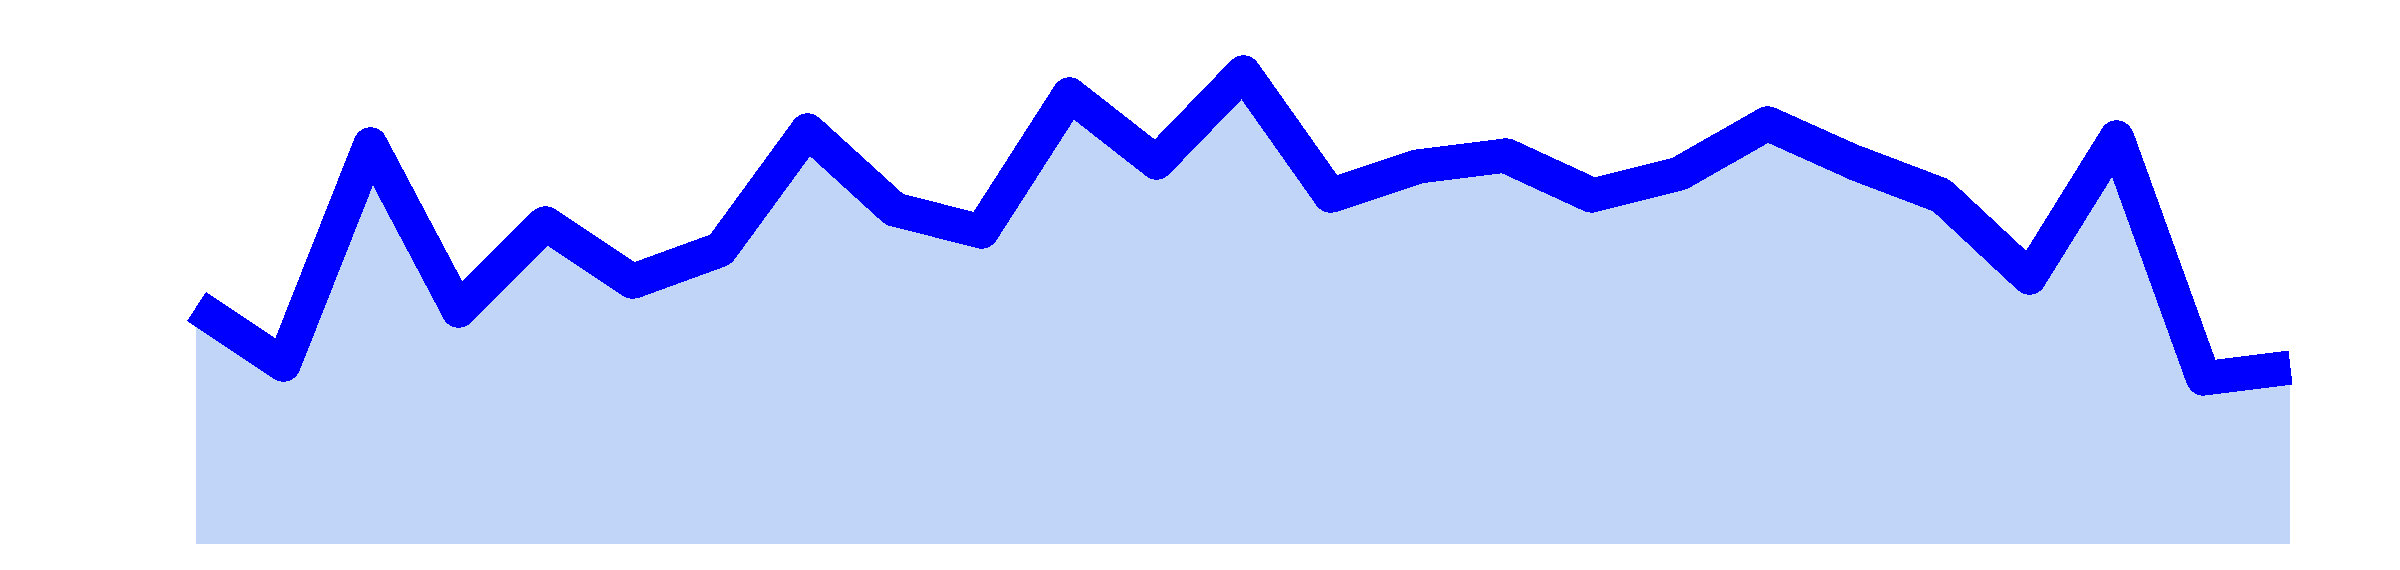
\includegraphics[width=2cm]{fig1.png}} & 0 & 0 & 163 & 162 & 554 & 72 & 49 & 49 & 49 & 49 & 72 & 0.43 & 536 & 569\\
2 & 932 & 454 & \raisebox{.12\height} {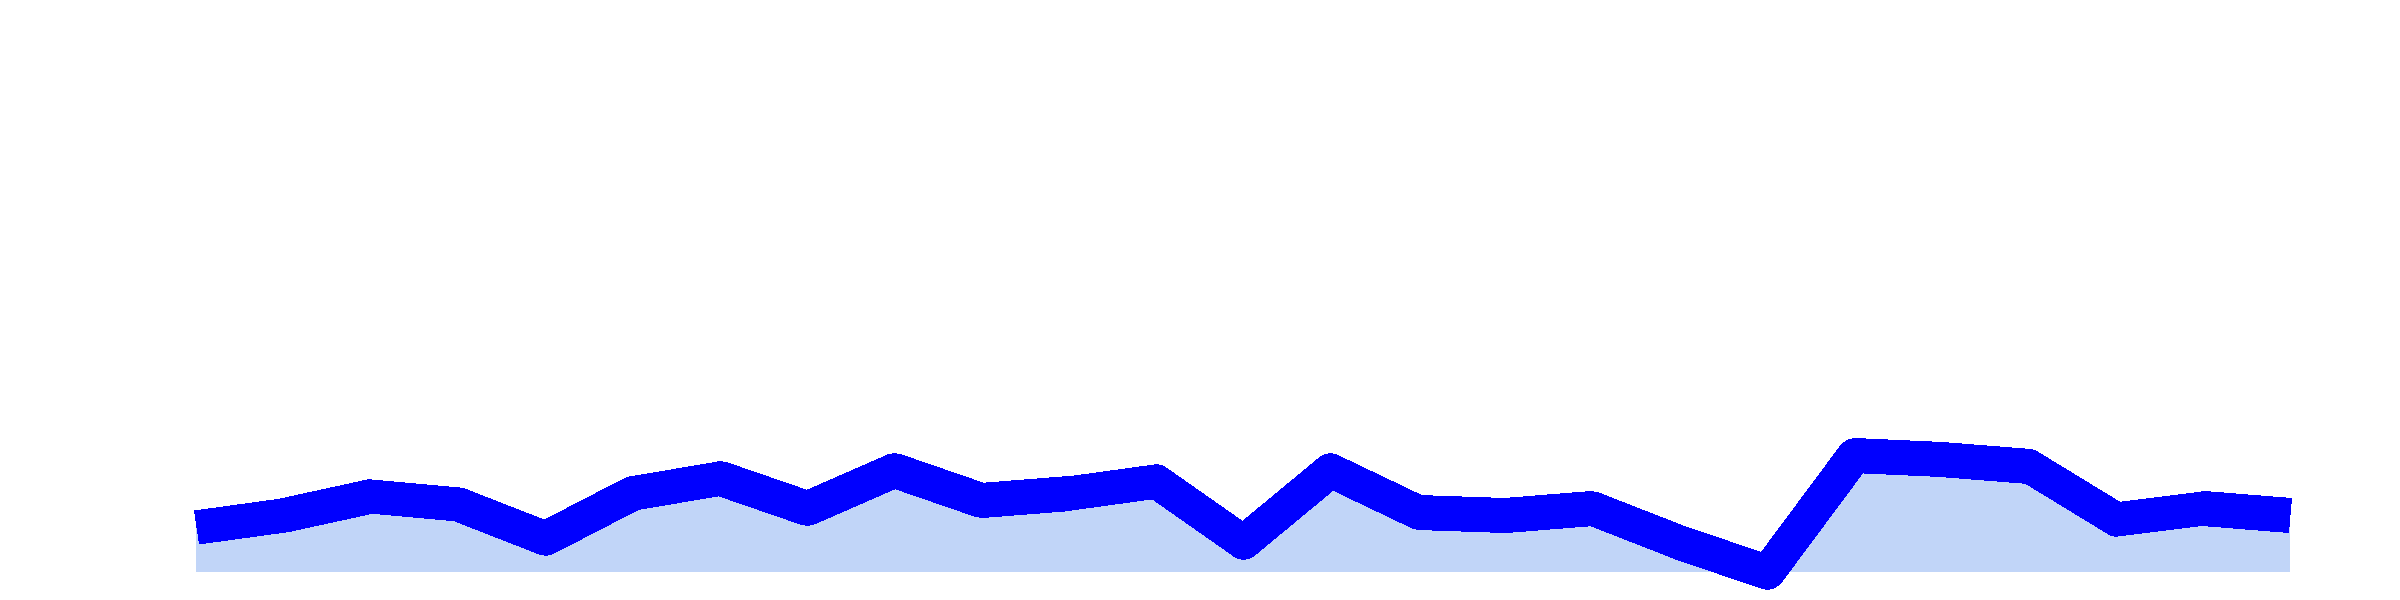
\includegraphics[width=2cm]{fig2.png}} & 1 & 0 & 126 & 127 & 575 & 48 & 48 & 48 & 48 & 48 & 48 & 0.46 & 541 & 589\\
3 & 748 & 287 & \raisebox{.12\height} {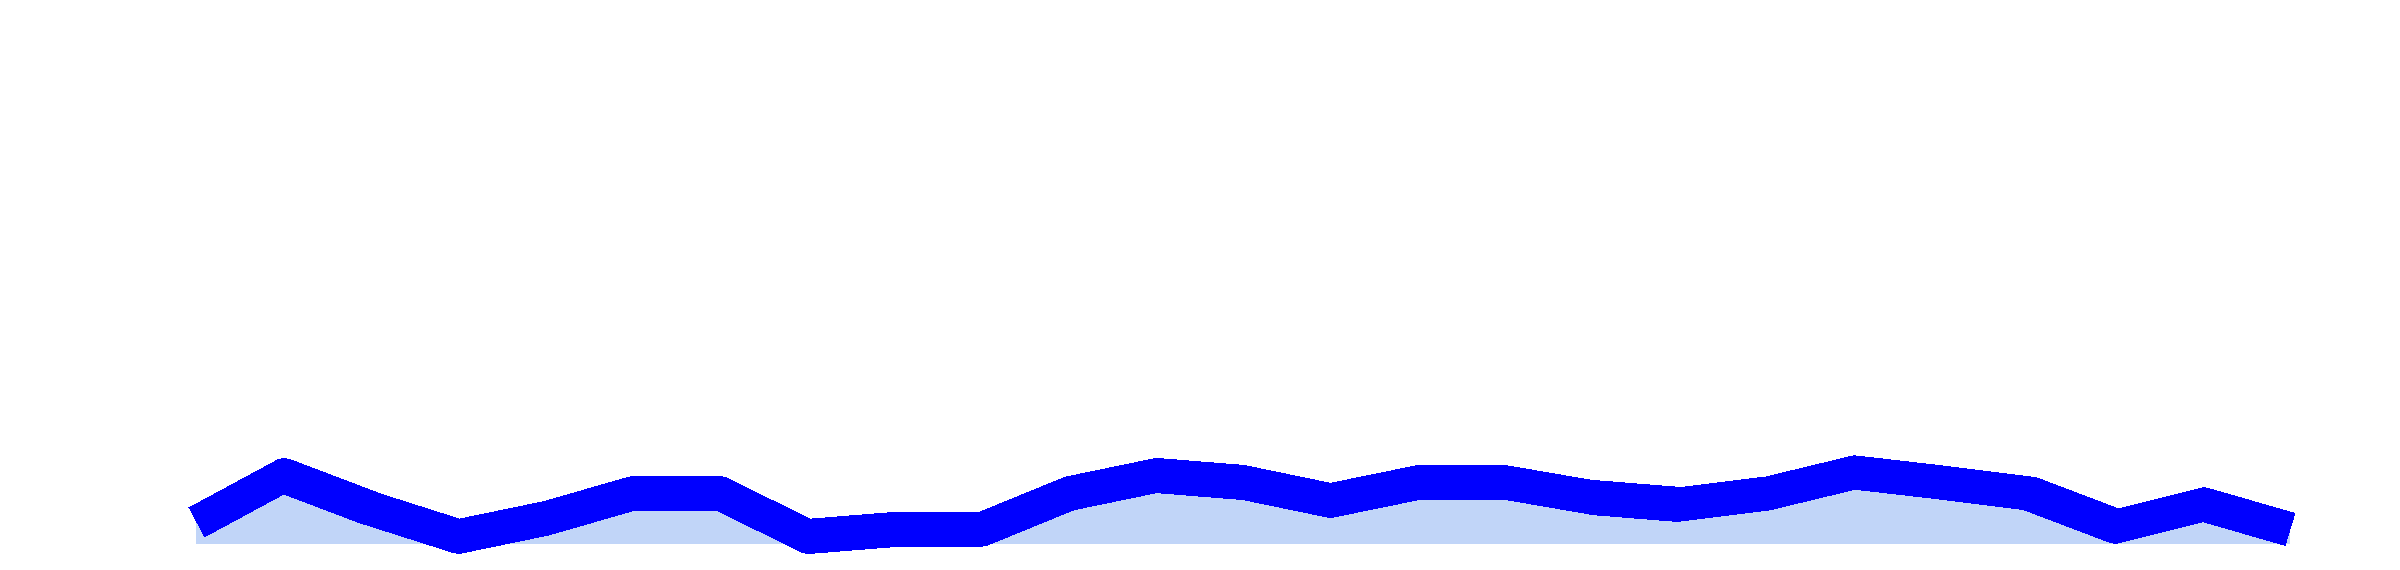
\includegraphics[width=2cm]{fig3.png}} & 0 & 0 & 91 & 91 & 619 & 43 & 43 & 43 & 43 & 43 & 43 & 0.19 & 568 & 636\\
4 & 2389 & 1355 & \raisebox{.12\height} {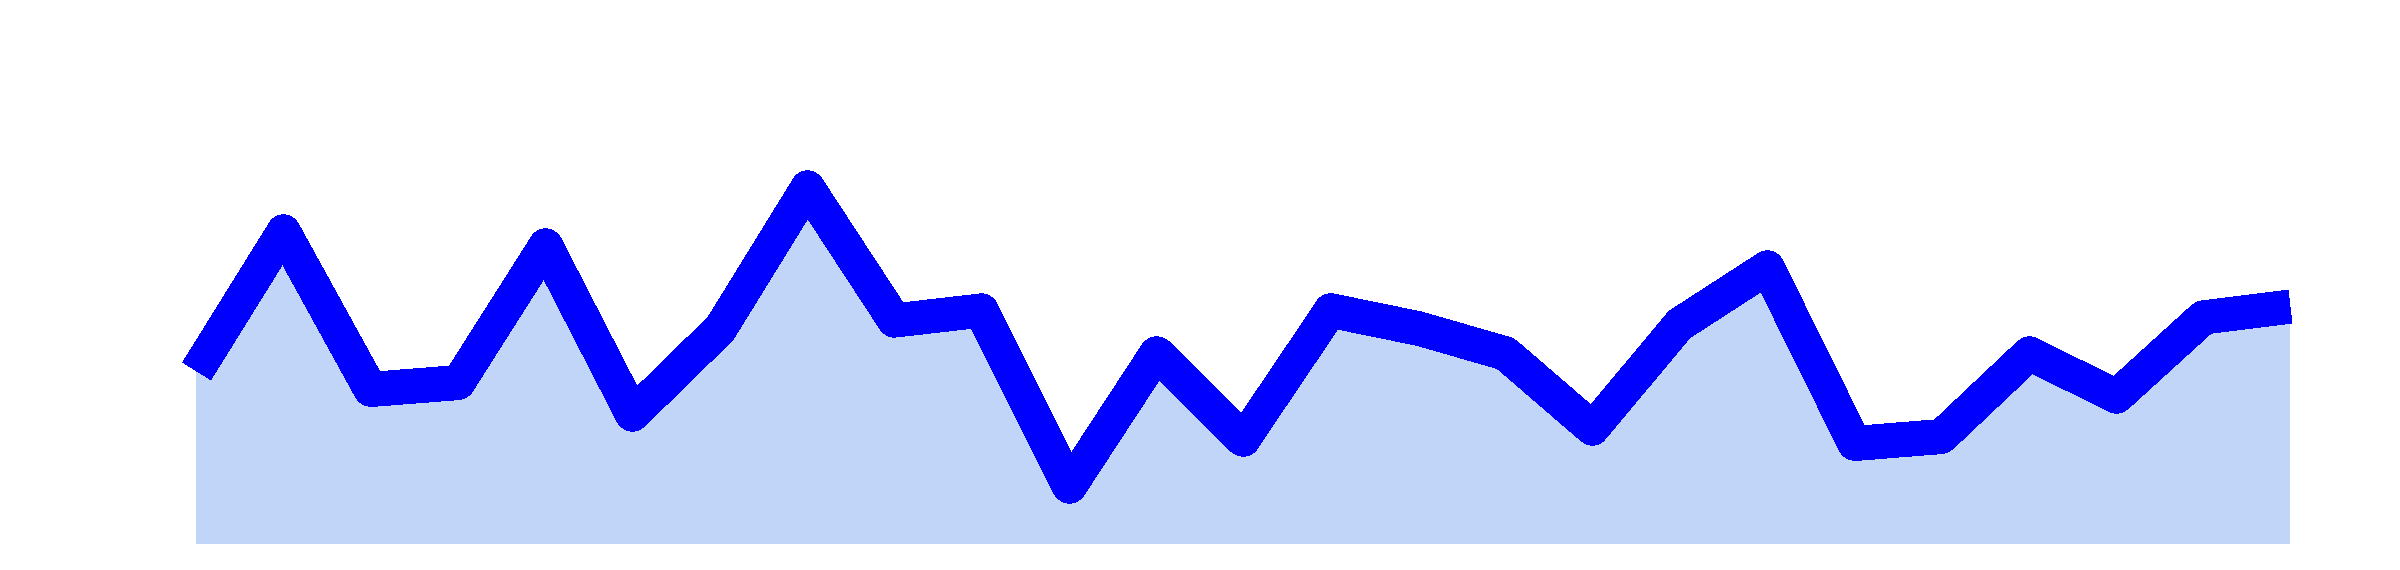
\includegraphics[width=2cm]{fig4.png}} & 0 & 0 & 156 & 155 & 554 & 50 & 50 & 50 & 50 & 50 & 50 & 0.40 & 557 & 583\\
5 & 2960 & 1625 & \raisebox{.12\height} {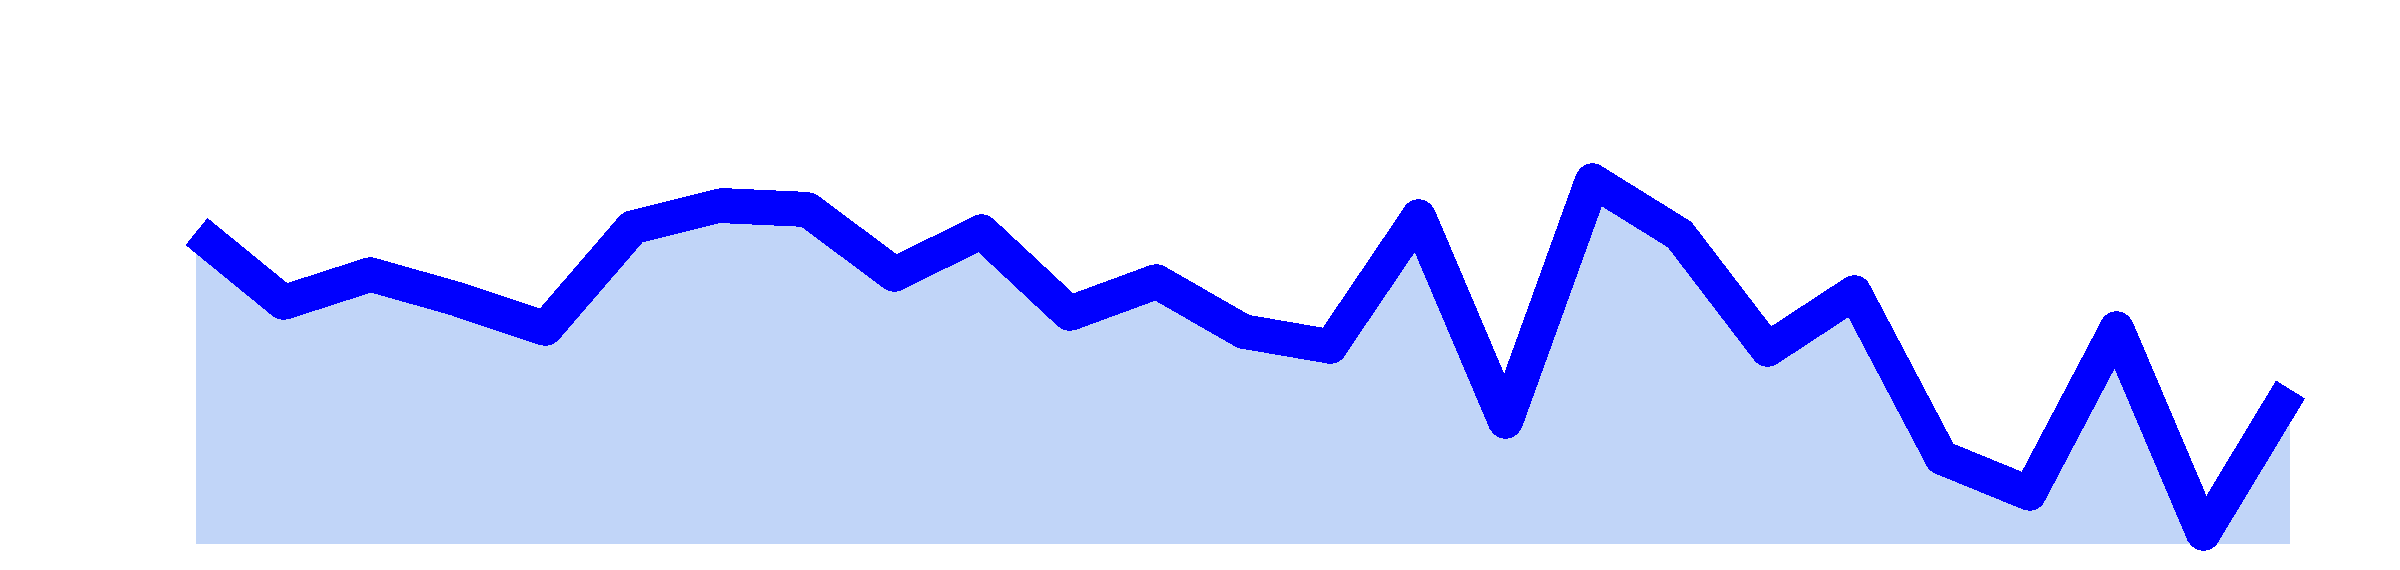
\includegraphics[width=2cm]{fig5.png}} & 0 & 0 & 116 & 116 & 556 & 48 & 41 & 41 & 41 & 41 & 48 & 0.51 & 541 & 583\\
6 & 917 & 372 & \raisebox{.12\height} {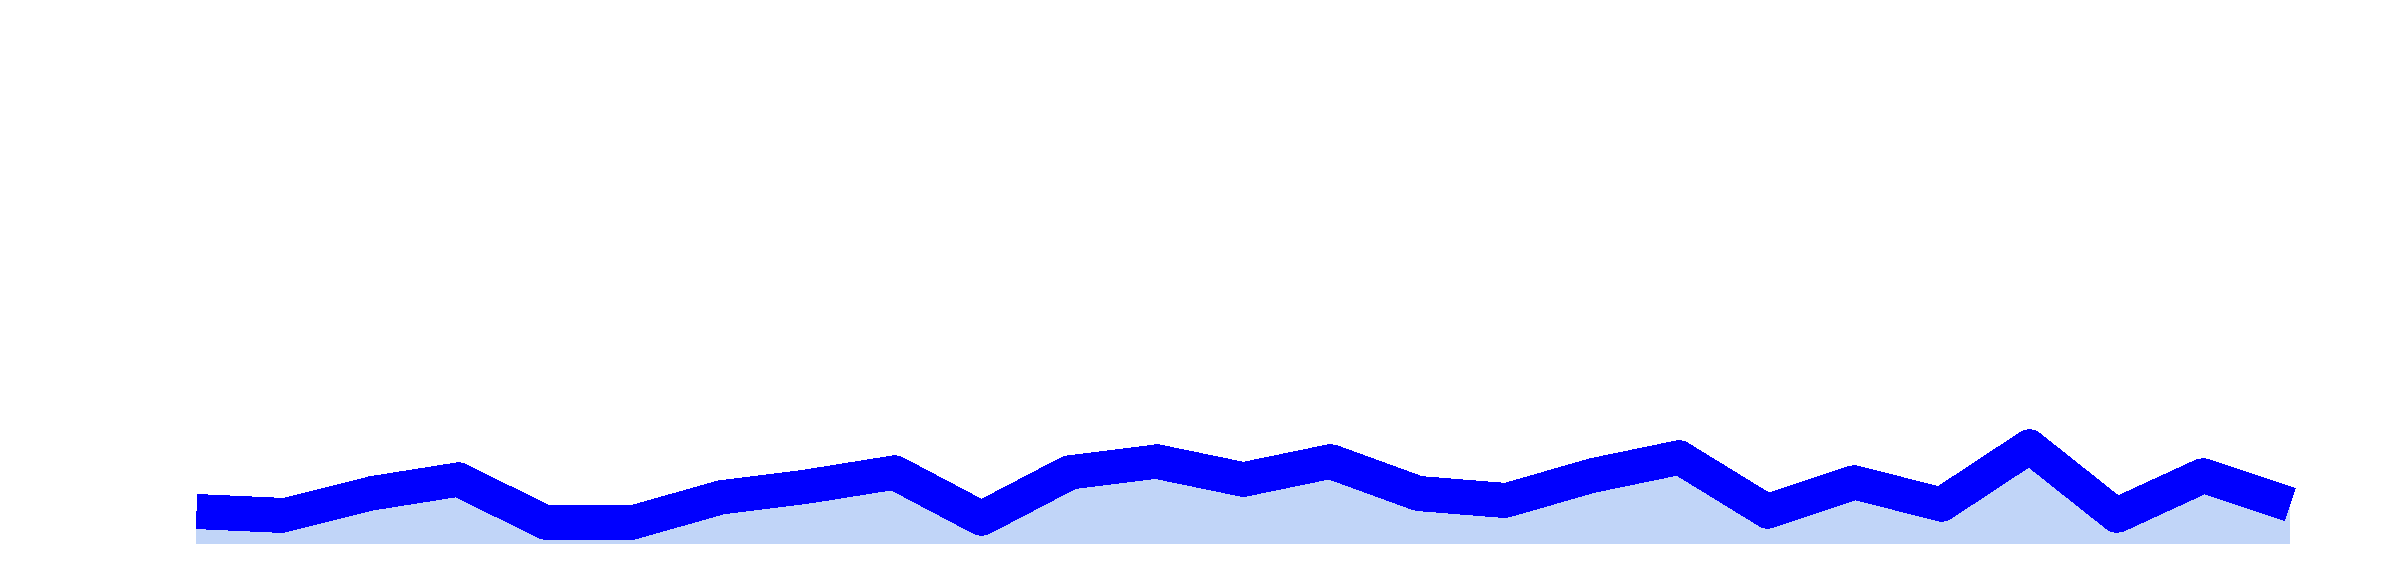
\includegraphics[width=2cm]{fig6.png}} & 2 & 0 & 115 & 117 & 617 & 44 & 46 & 46 & 46 & 46 & 47 & 0.17 & 599 & 615\\
7 & 573 & 214 & \raisebox{.12\height} {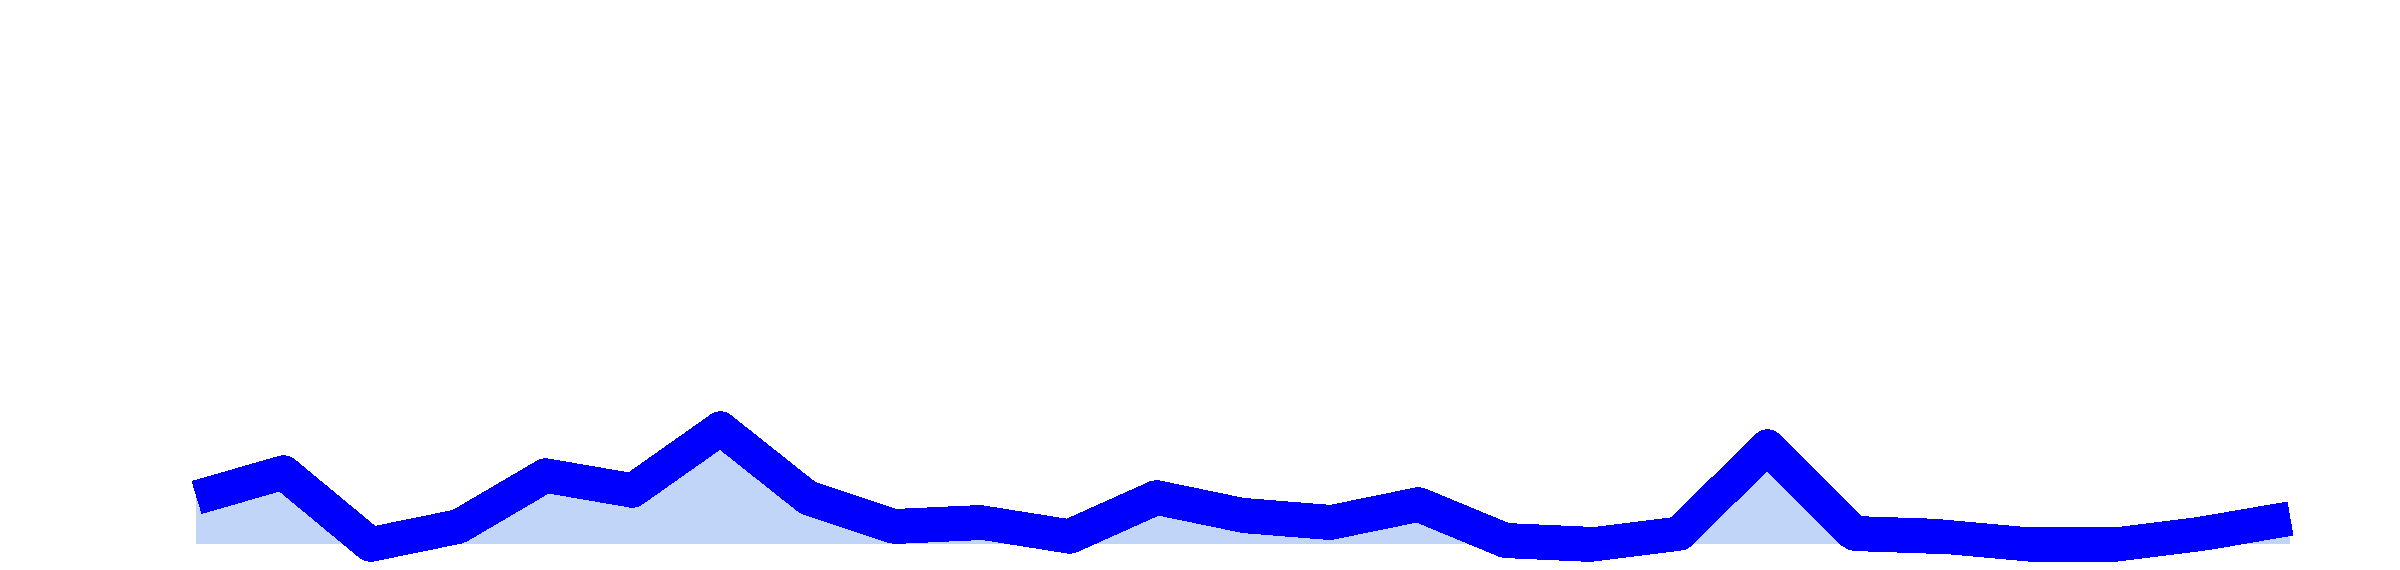
\includegraphics[width=2cm]{fig7.png}} & 1 & 0 & 97 & 98 & 606 & 45 & 45 & 45 & 45 & 45 & 46 & 0.07 & 580 & 627\\
8 & 20 & 6 & \raisebox{.12\height} {
\includegraphics[width=2cm]{fig8.png}} & 0 & 0 & 1 & 1 & 601 & 1 & 1 & 1 & 1 & 1 & 1 & 0.00 & 0 & 745\\
9 & 1159 & 788 & \raisebox{.12\height} {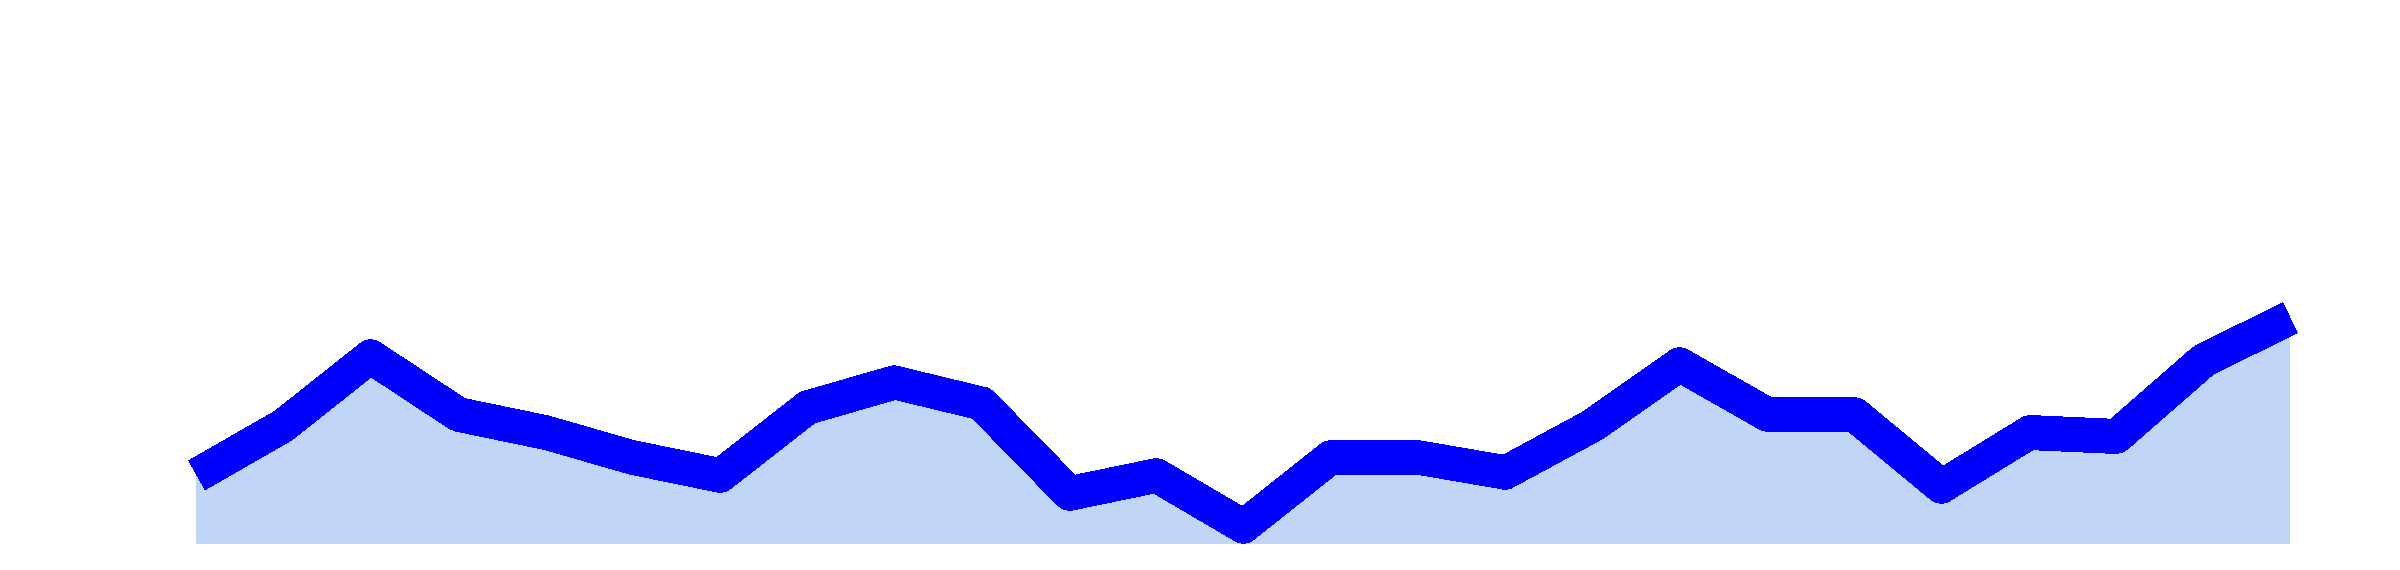
\includegraphics[width=2cm]{fig9.png}} & 1 & 0 & 140 & 140 & 518 & 57 & 57 & 57 & 56 & 57 & 61 & 0.74 & 516 & 539\\
10 & 1970 & 1032 & \raisebox{.12\height} {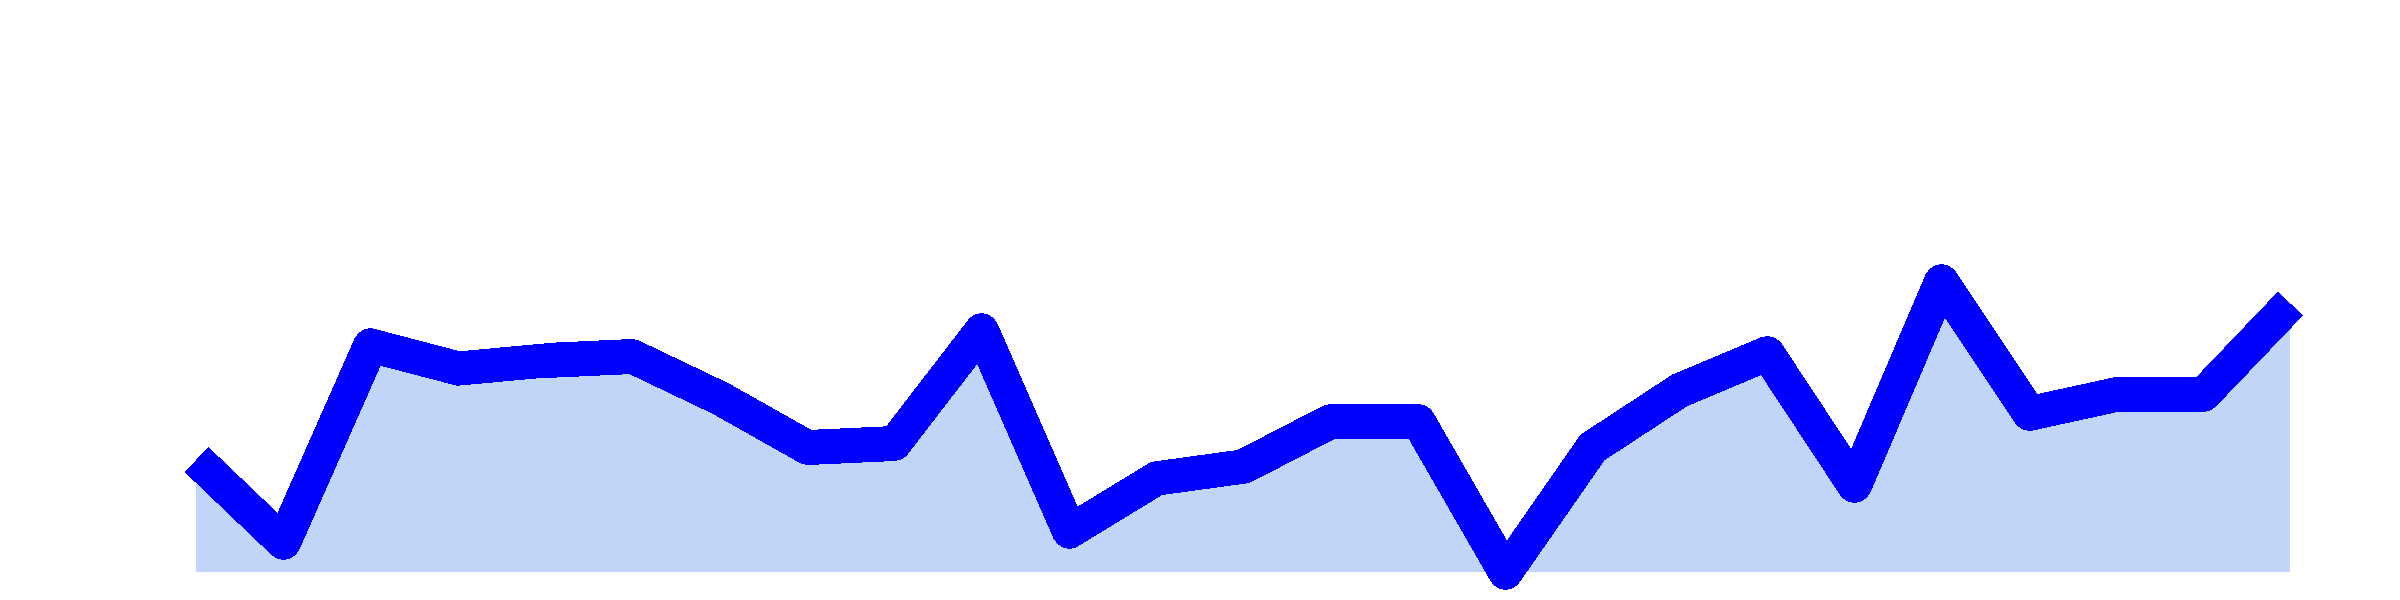
\includegraphics[width=2cm]{fig10.png}} & 0 & 0 & 112 & 112 & 572 & 54 & 53 & 54 & 54 & 54 & 54 & 0.23 & 561 & 590\\
11 & 2192 & 1230 & \raisebox{.12\height} {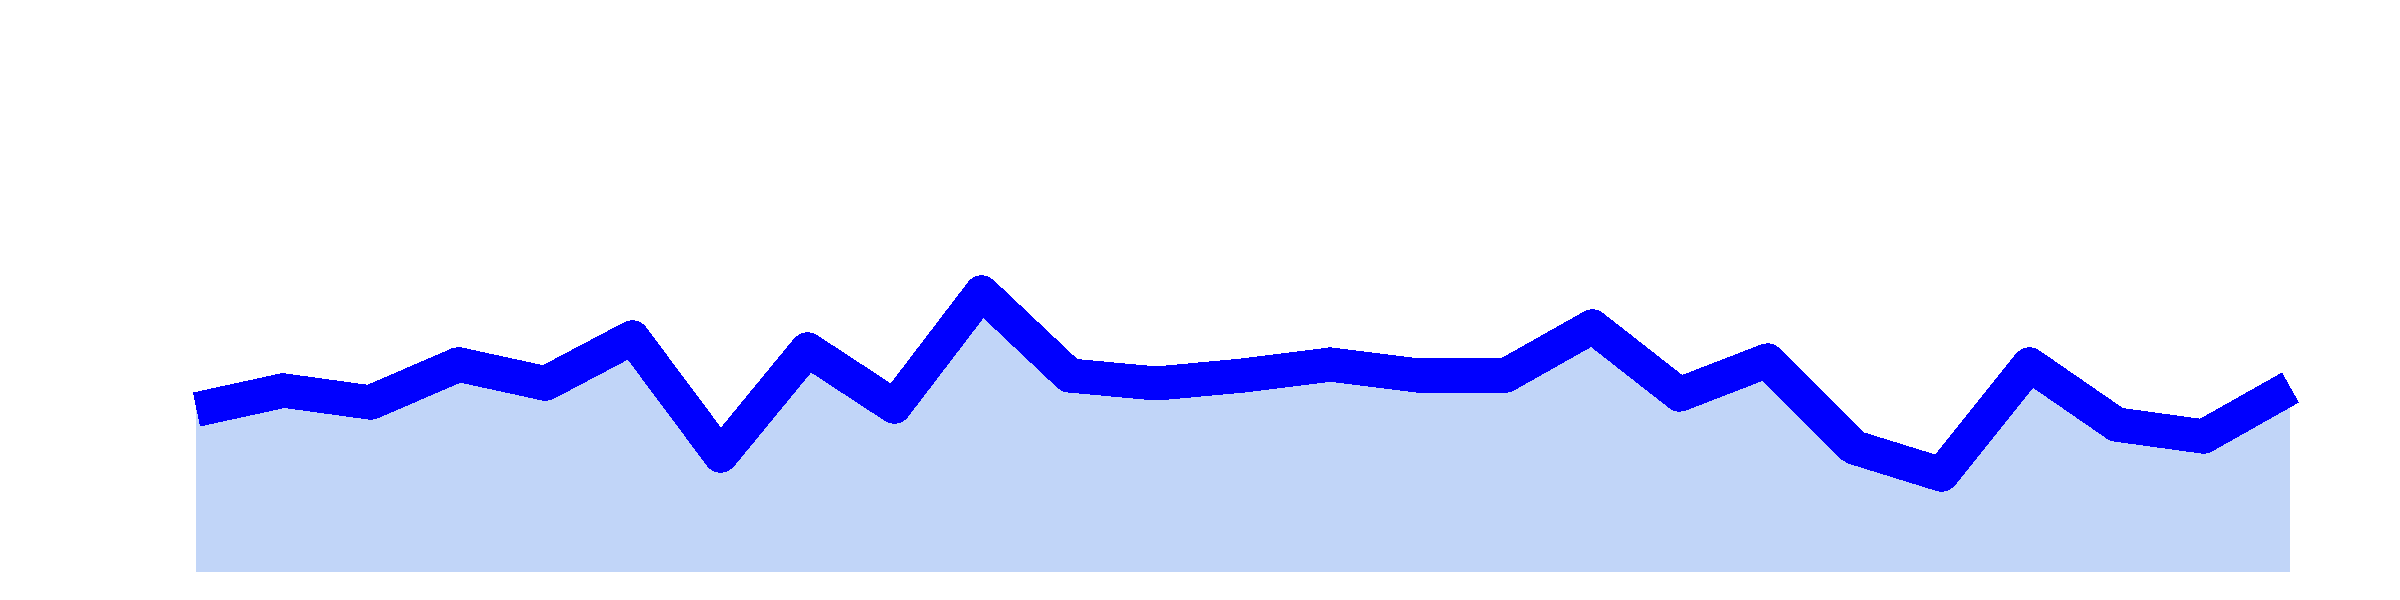
\includegraphics[width=2cm]{fig11.png}} & 0 & 0 & 159 & 159 & 539 & 54 & 54 & 54 & 54 & 54 & 54 & 0.74 & 518 & 582\\
12 & 1545 & 717 & \raisebox{.12\height} {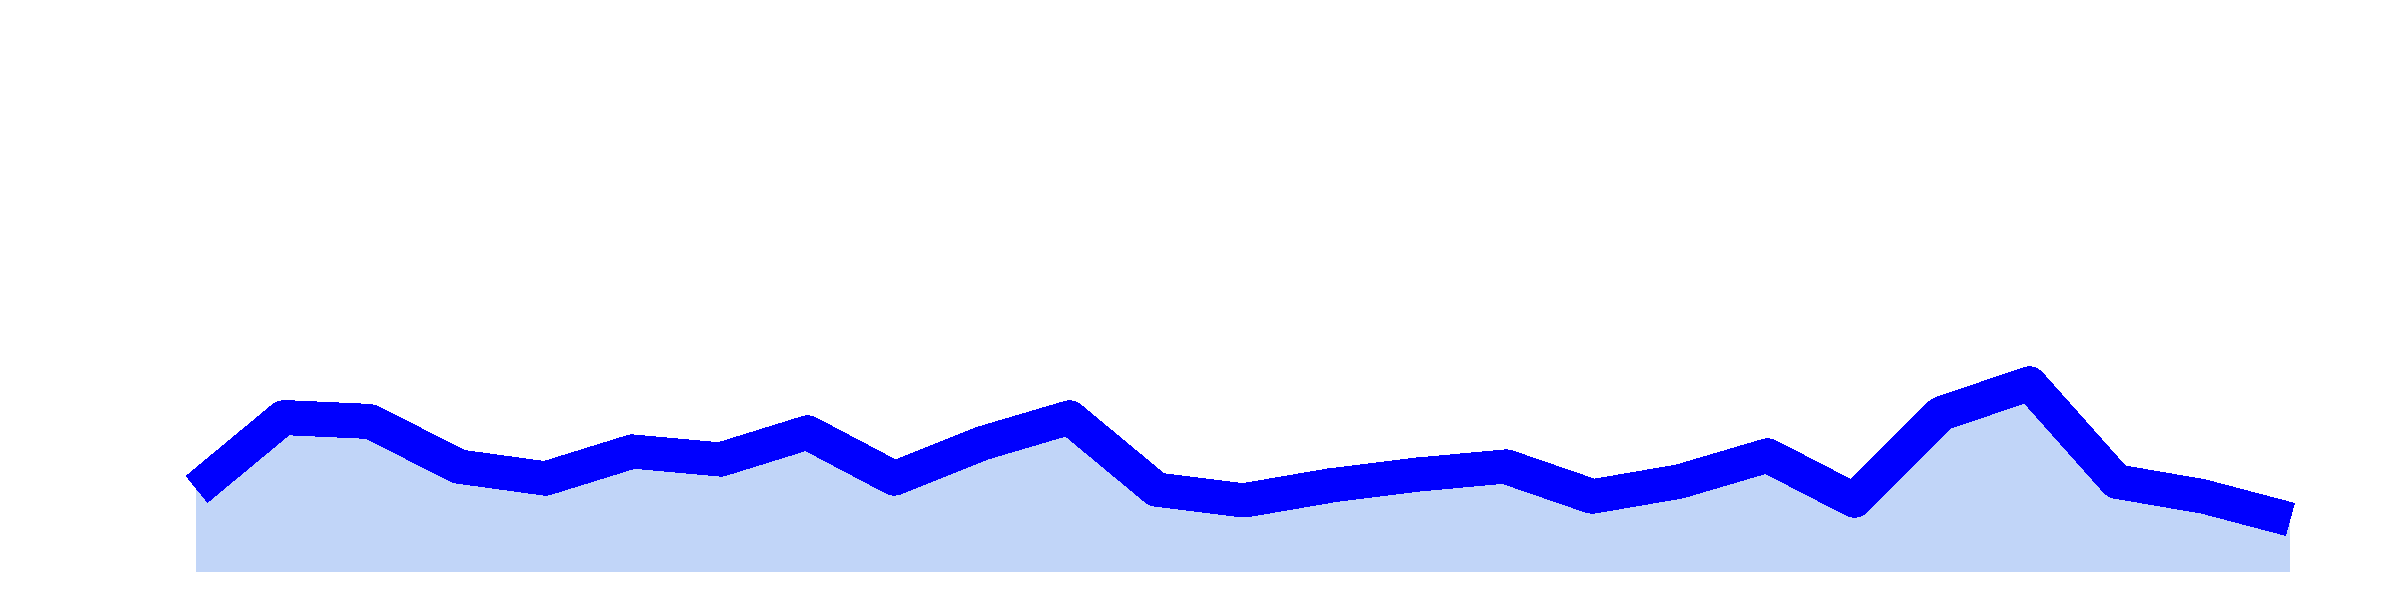
\includegraphics[width=2cm]{fig12.png}} & 2 & 0 & 121 & 123 & 602 & 50 & 49 & 49 & 49 & 49 & 50 & 0.45 & 535 & 596\\
13 & 2128 & 1283 & \raisebox{.12\height} {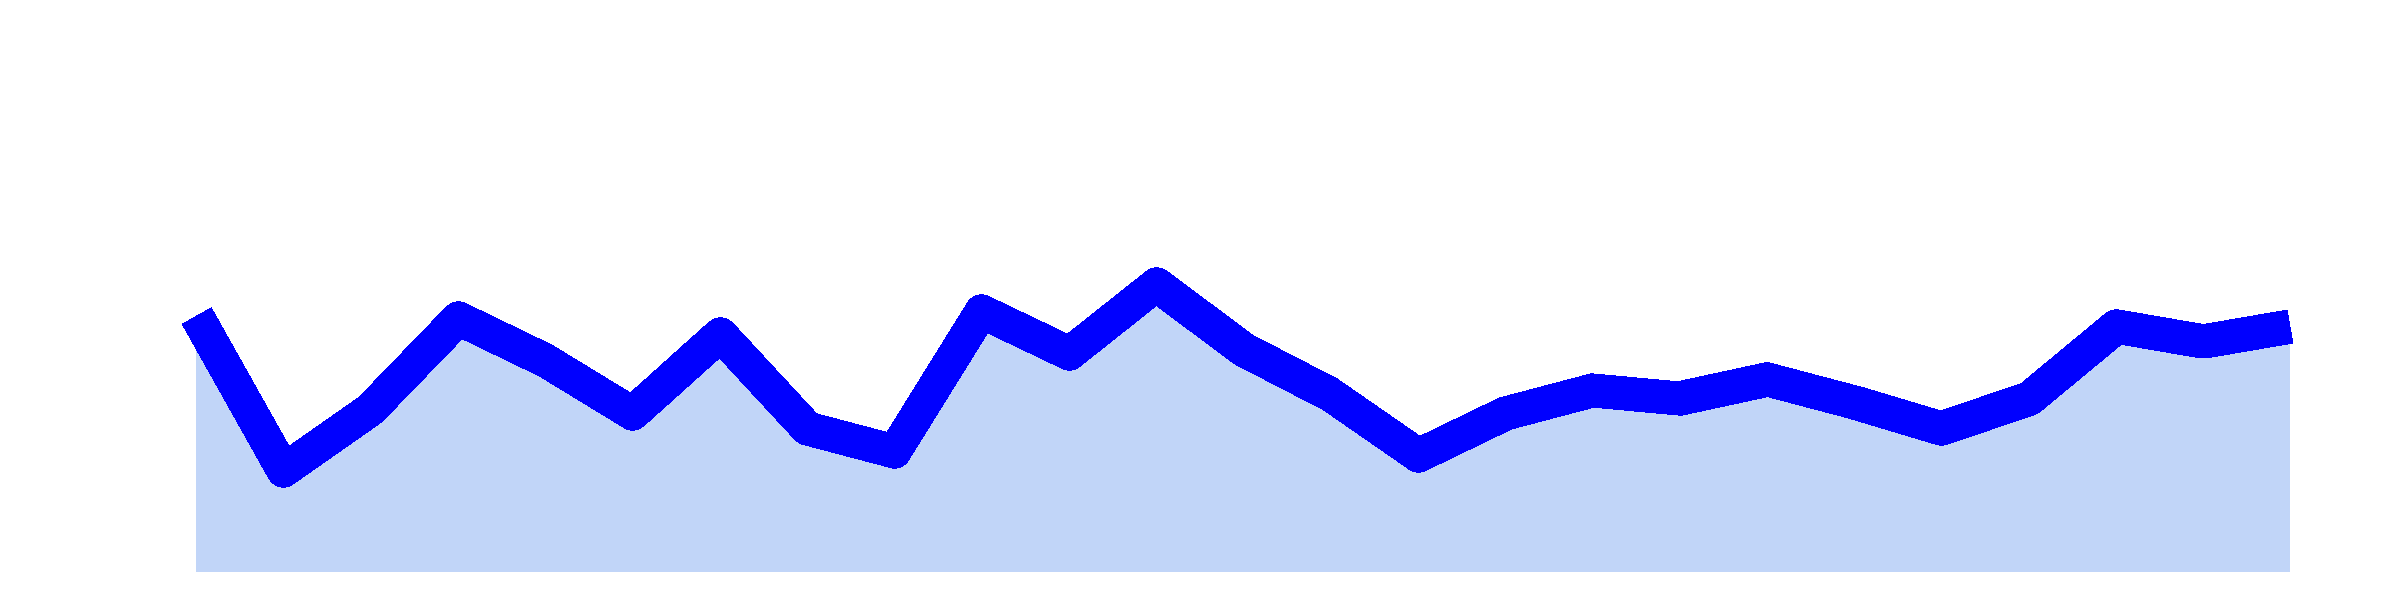
\includegraphics[width=2cm]{fig13.png}} & 2 & 0 & 127 & 129 & 535 & 50 & 50 & 50 & 50 & 49 & 50 & 0.50 & 526 & 566\\
14 & 2053 & 1160 & \raisebox{.12\height} {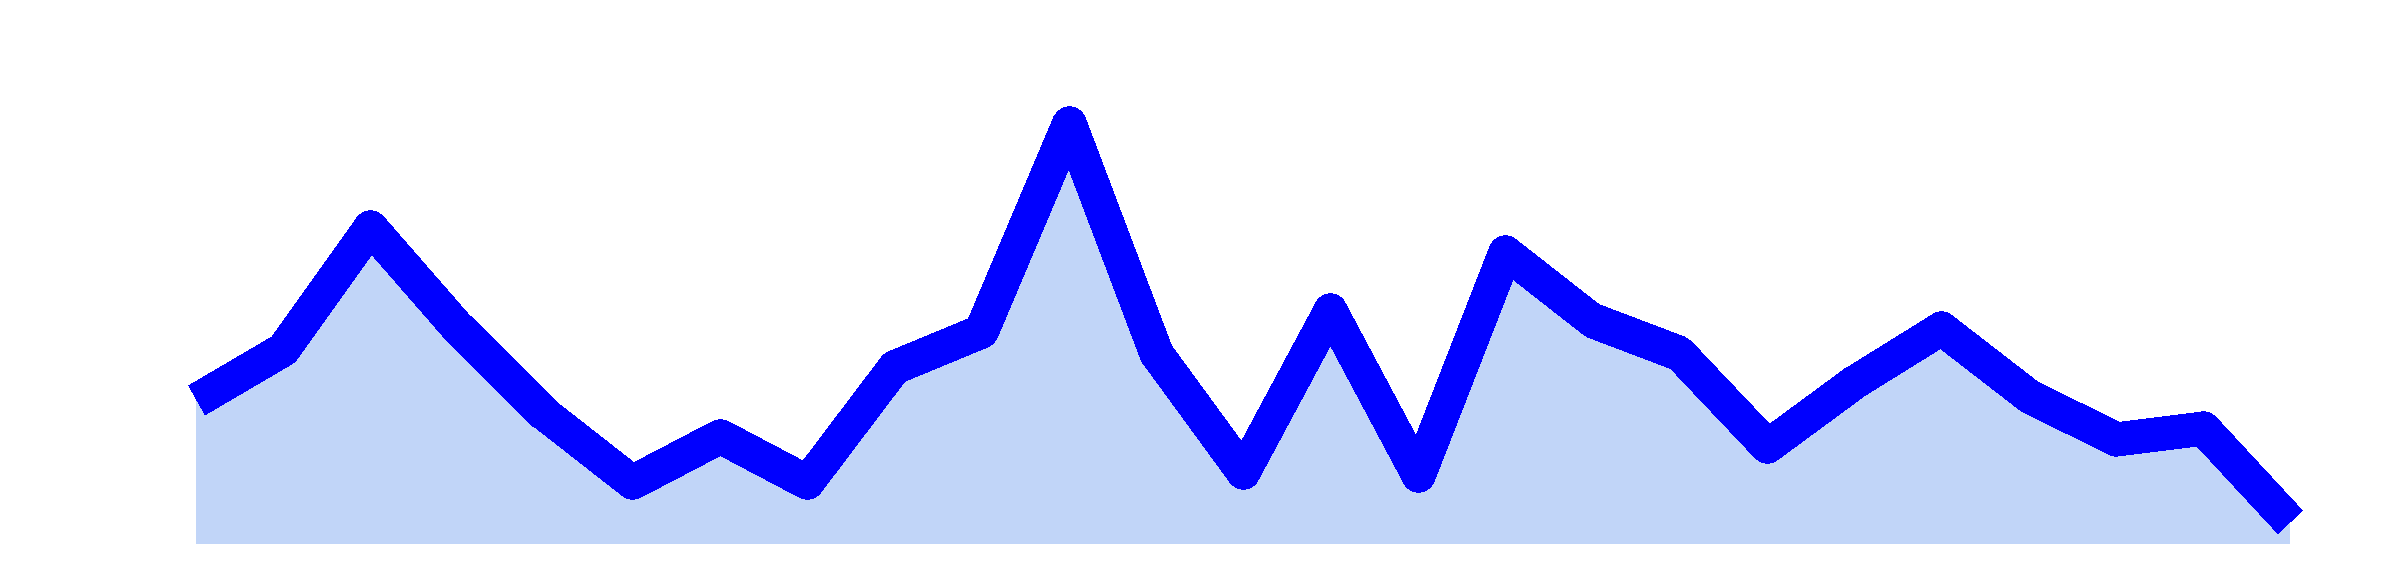
\includegraphics[width=2cm]{fig14.png}} & 1 & 0 & 113 & 114 & 545 & 61 & 61 & 61 & 61 & 61 & 61 & 0.39 & 543 & 573\\
15 & 1738 & 1155 & \raisebox{.12\height} {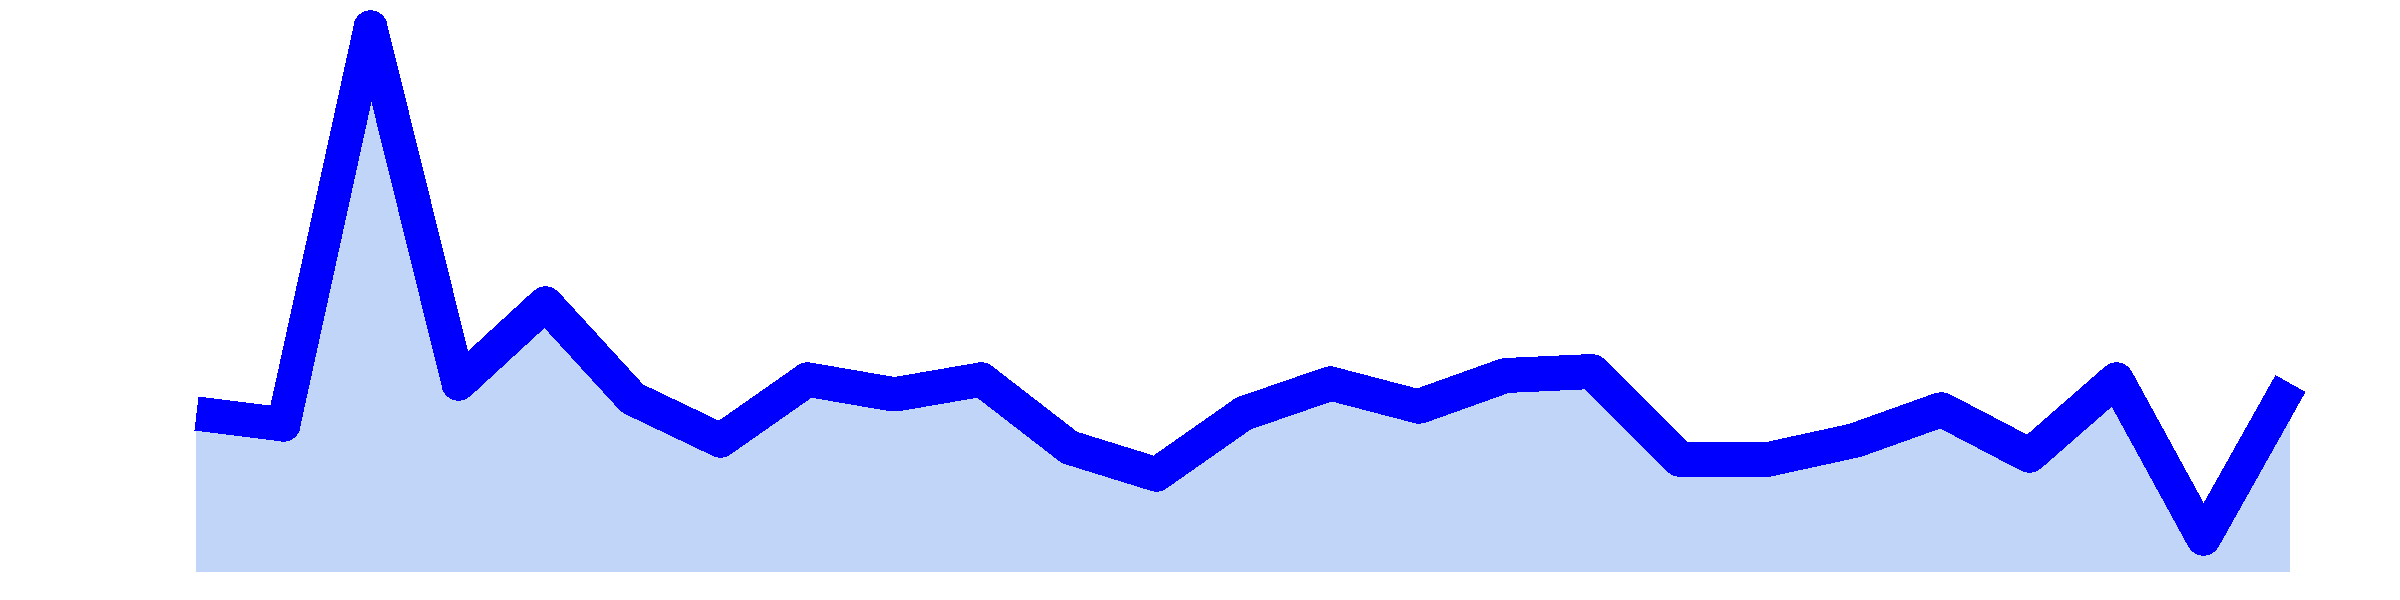
\includegraphics[width=2cm]{fig15.png}} & 2 & 0 & 144 & 146 & 528 & 57 & 57 & 57 & 57 & 57 & 57 & 0.63 & 509 & 514\\
16 & 1236 & 915 & \raisebox{.12\height} {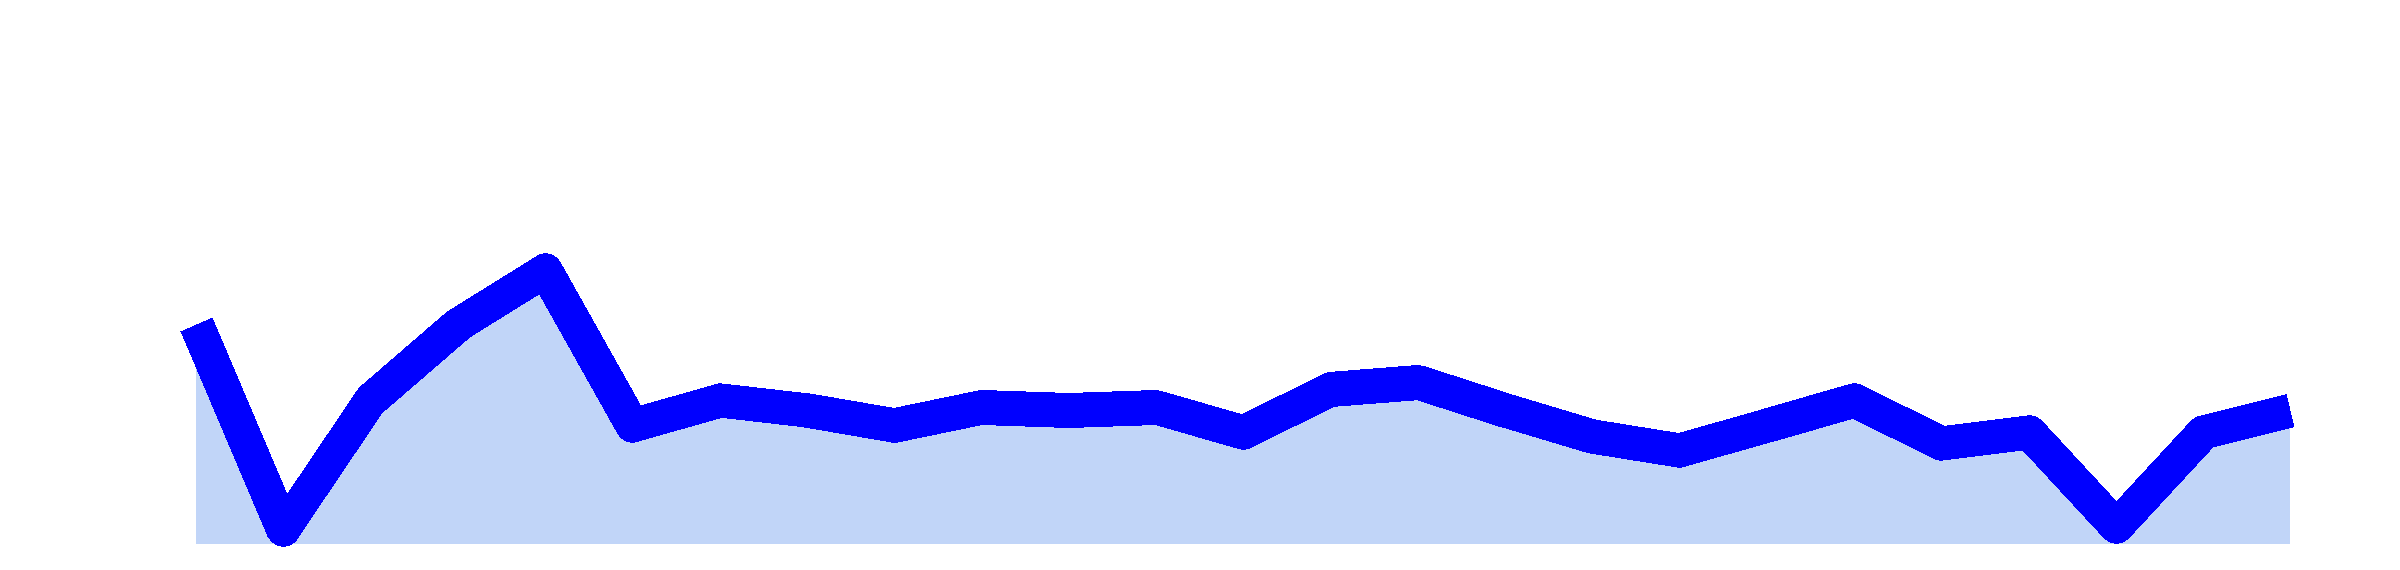
\includegraphics[width=2cm]{fig16.png}} & 0 & 0 & 152 & 152 & 503 & 46 & 46 & 46 & 46 & 46 & 46 & 0.74 & 499 & 508\\
17 & 1011 & 642 & \raisebox{.12\height} {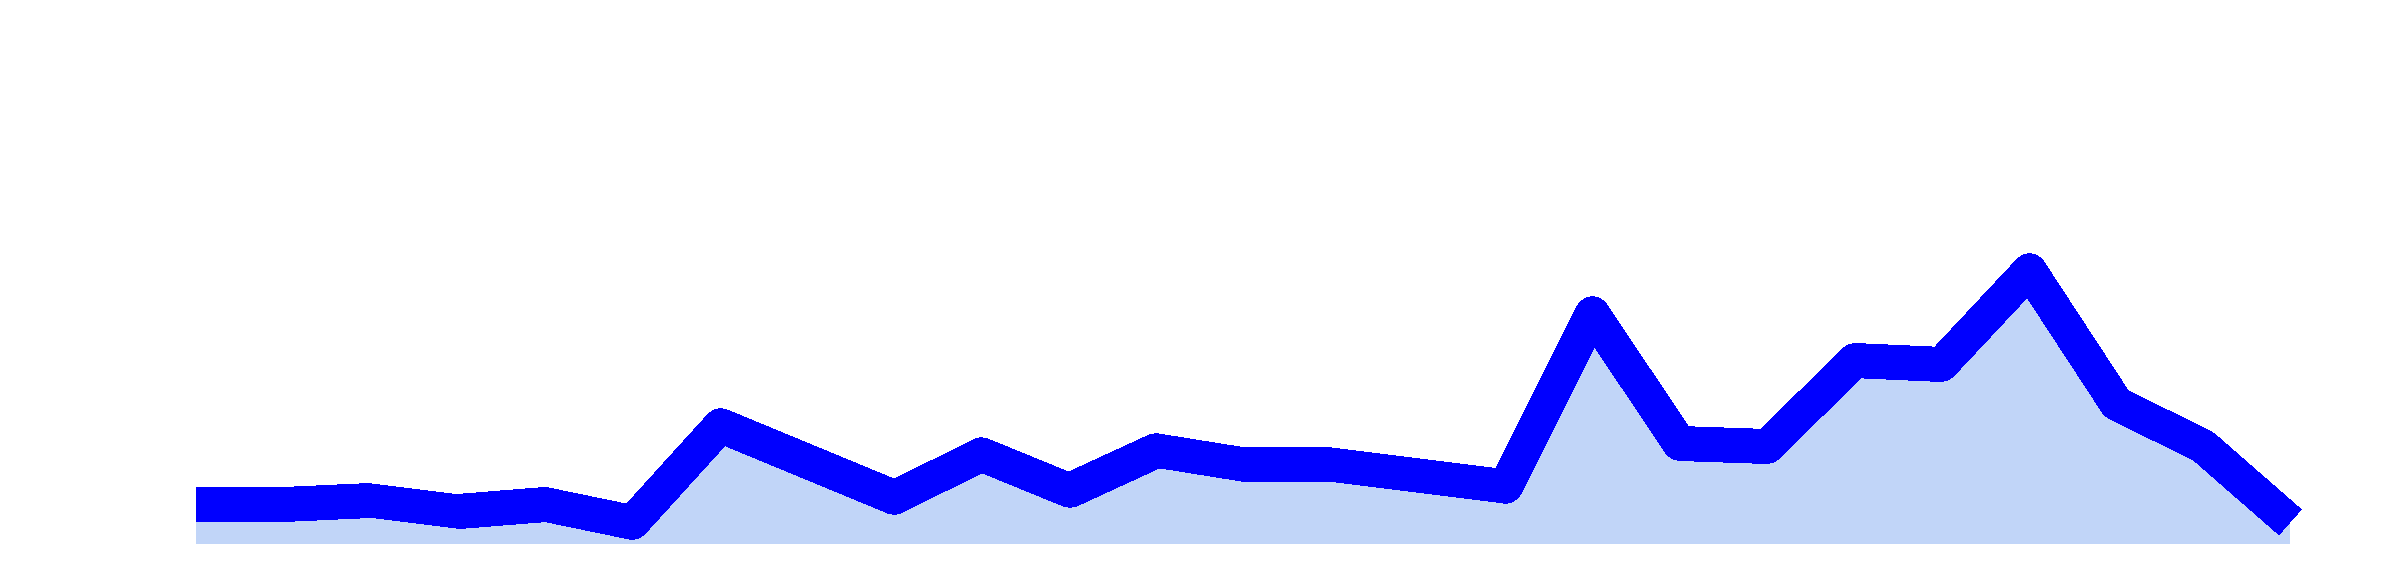
\includegraphics[width=2cm]{fig17.png}} & 0 & 0 & 115 & 115 & 524 & 58 & 57 & 57 & 56 & 57 & 58 & 0.70 & 511 & 550\\
18 & 2030 & 1033 & \raisebox{.12\height} {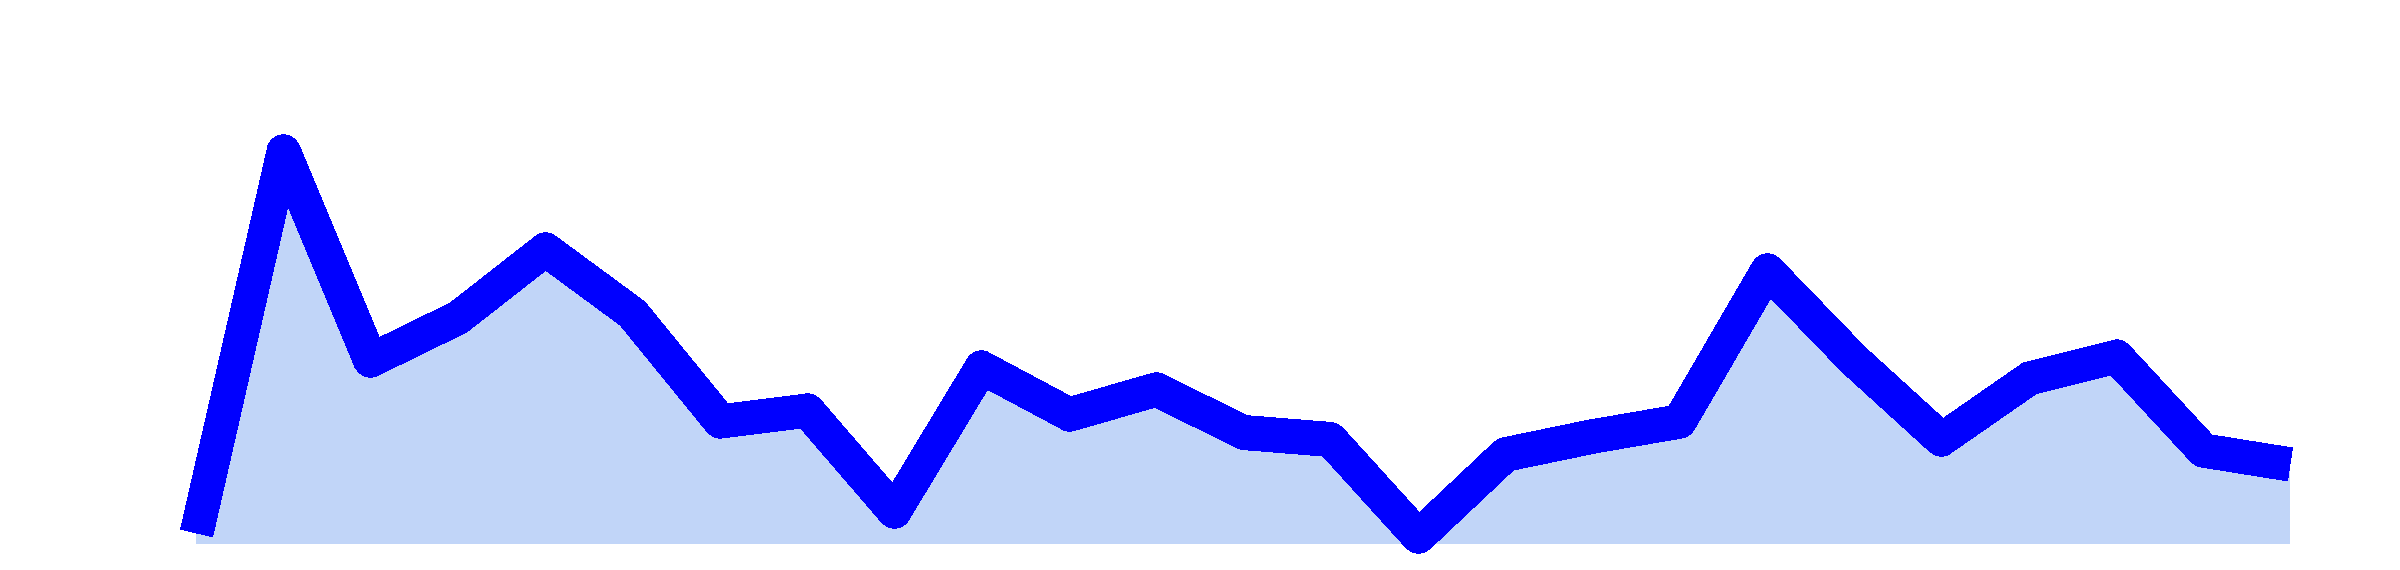
\includegraphics[width=2cm]{fig18.png}} & 0 & 0 & 124 & 124 & 563 & 54 & 54 & 54 & 54 & 54 & 54 & 0.39 & 545 & 579\\
19 & 1448 & 916 & \raisebox{.12\height} {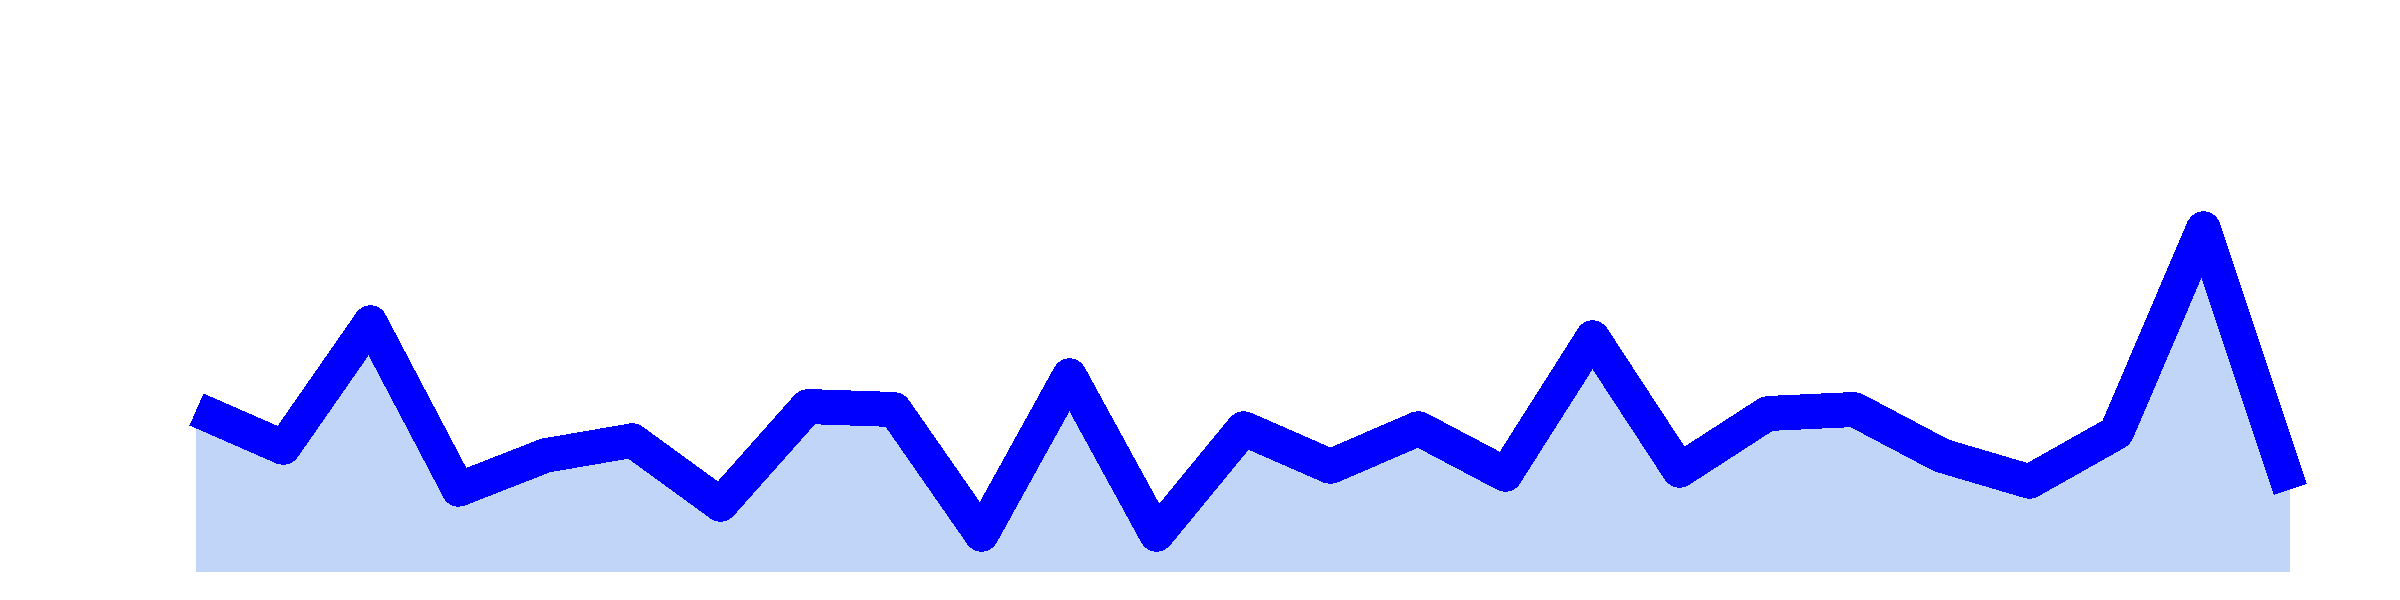
\includegraphics[width=2cm]{fig19.png}} & 0 & 0 & 127 & 127 & 522 & 48 & 48 & 48 & 47 & 48 & 48 & 0.67 & 514 & 545\\
20 & 1390 & 566 & \raisebox{.12\height} {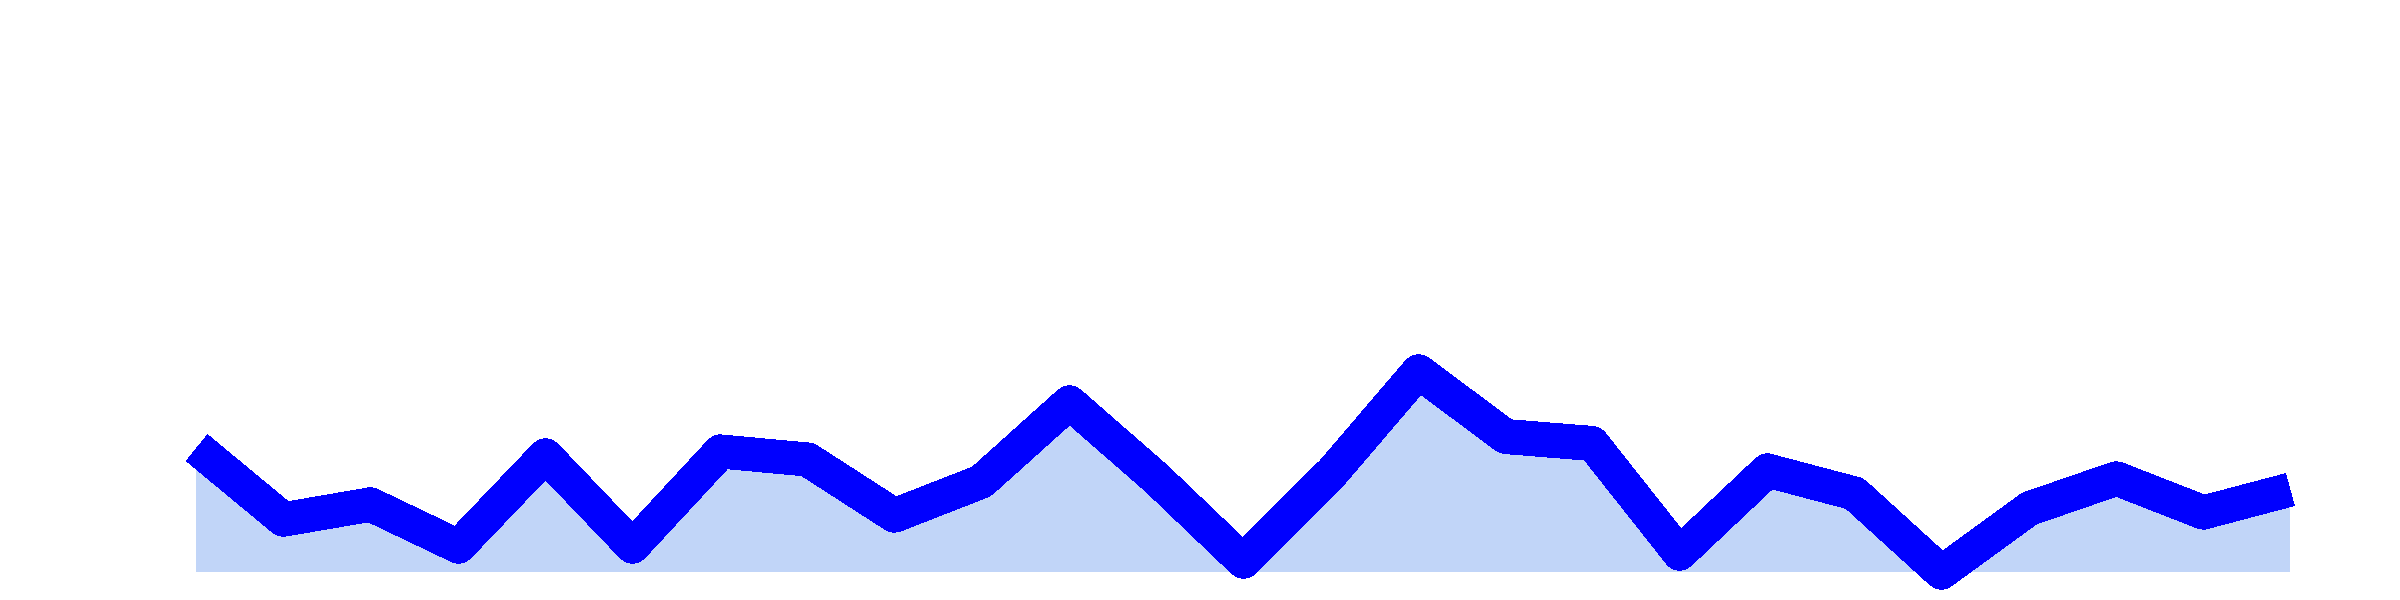
\includegraphics[width=2cm]{fig20.png}} & 1 & 0 & 135 & 136 & 600 & 52 & 52 & 52 & 52 & 52 & 52 & 0.37 & 573 & 623\\
21 & 772 & 294 & \raisebox{.12\height} {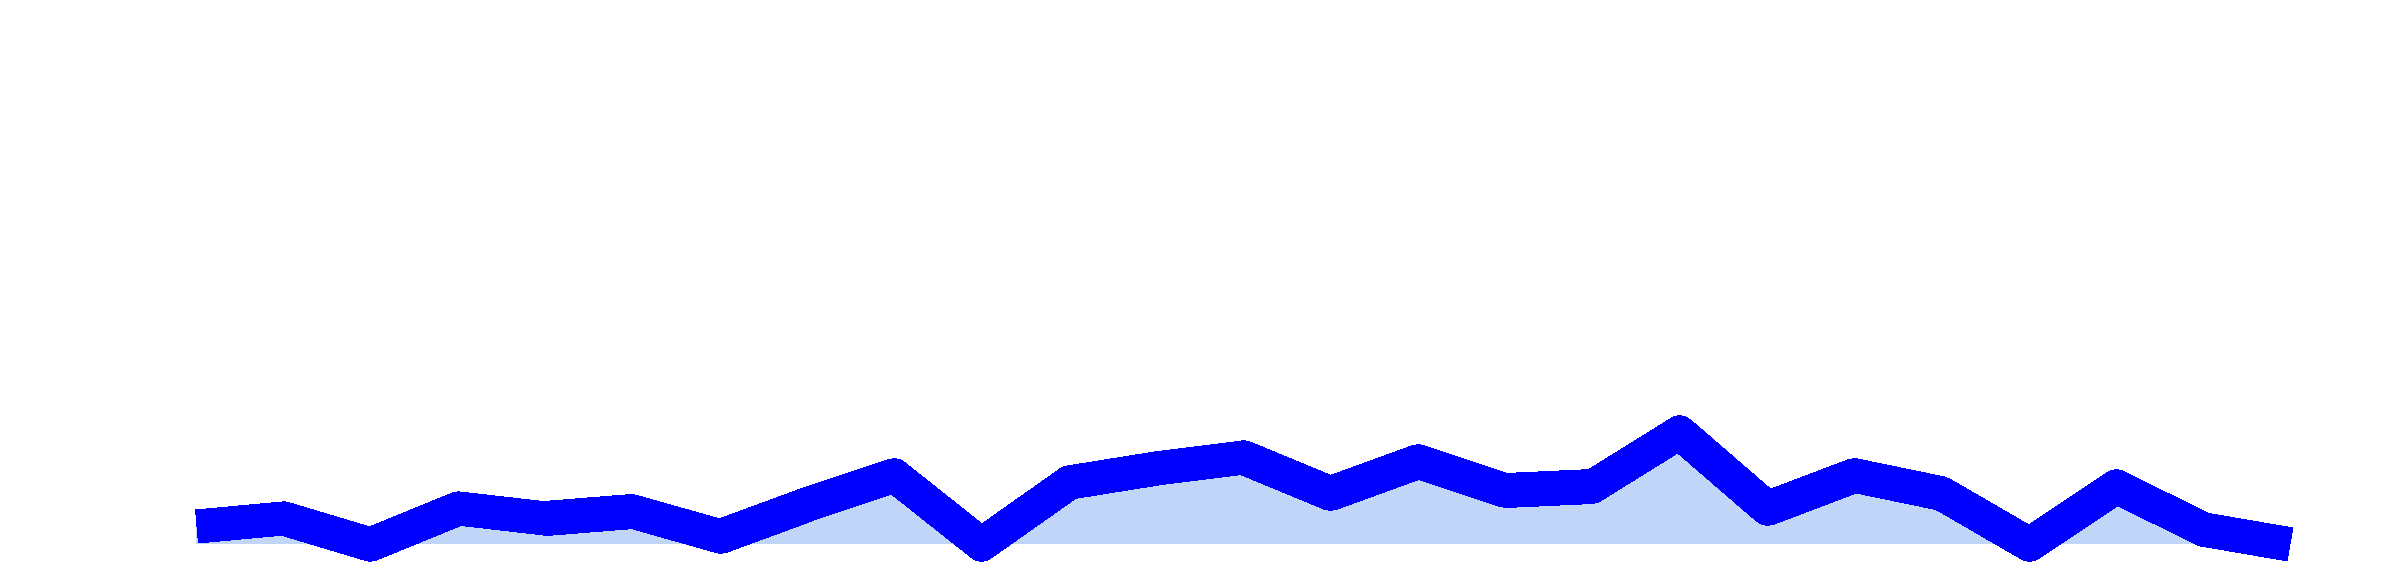
\includegraphics[width=2cm]{fig21.png}} & 2 & 0 & 66 & 68 & 624 & 48 & 48 & 48 & 48 & 48 & 48 & 0.42 & 569 & 629\\
22 & 480 & 244 & \raisebox{.12\height} {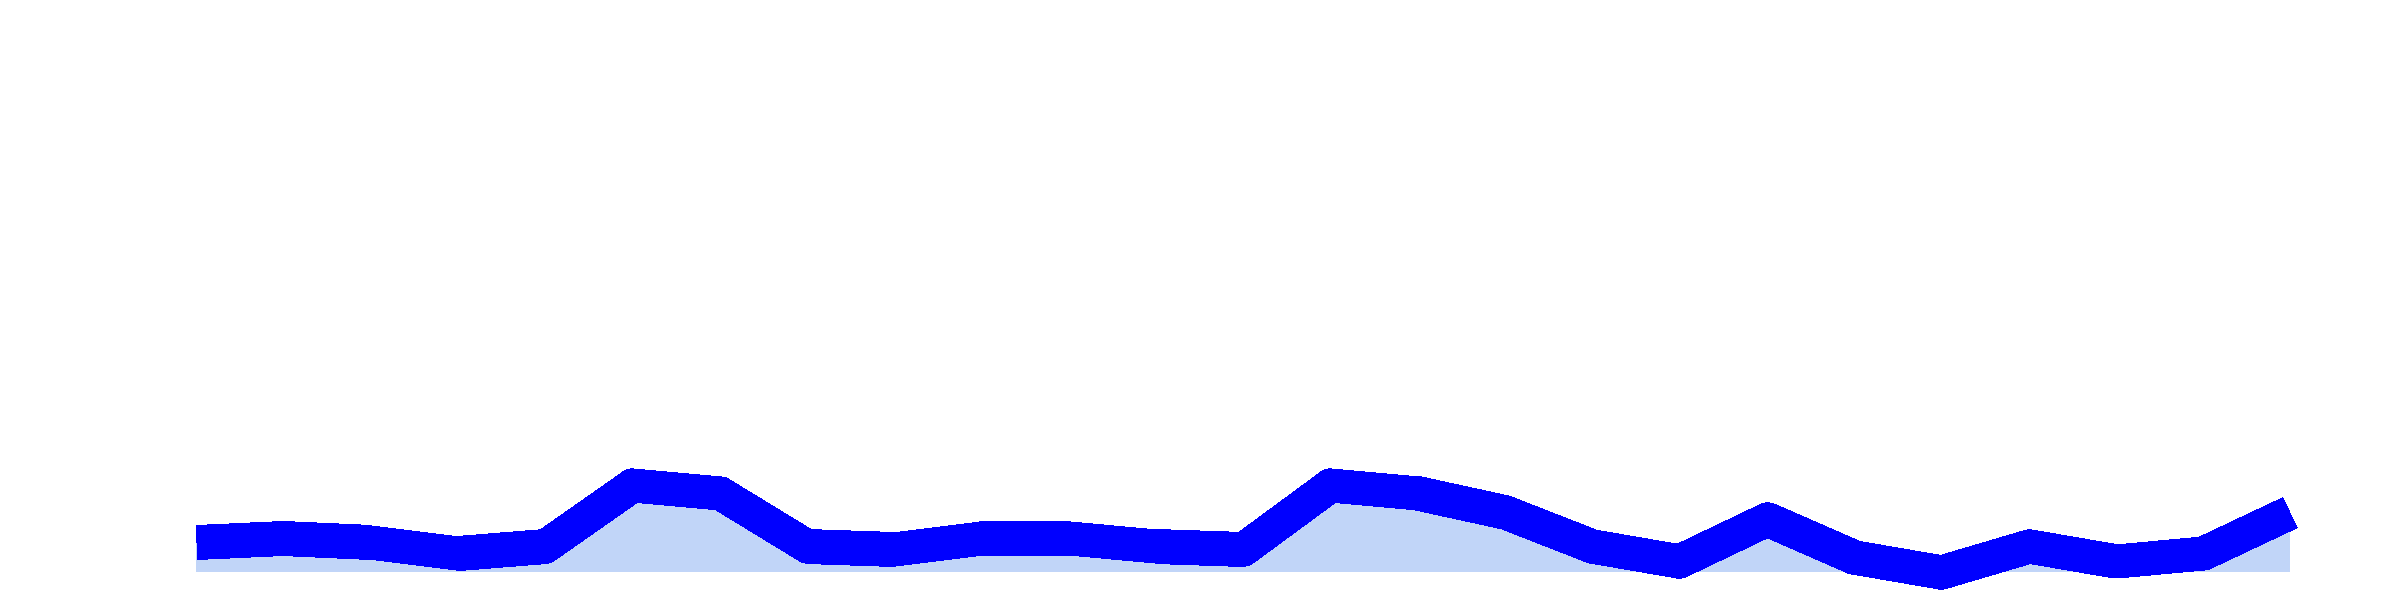
\includegraphics[width=2cm]{fig22.png}} & 1 & 0 & 72 & 73 & 568 & 55 & 55 & 55 & 55 & 55 & 55 & 0.69 & 558 & 631\\
23 & 977 & 403 & \raisebox{.12\height} {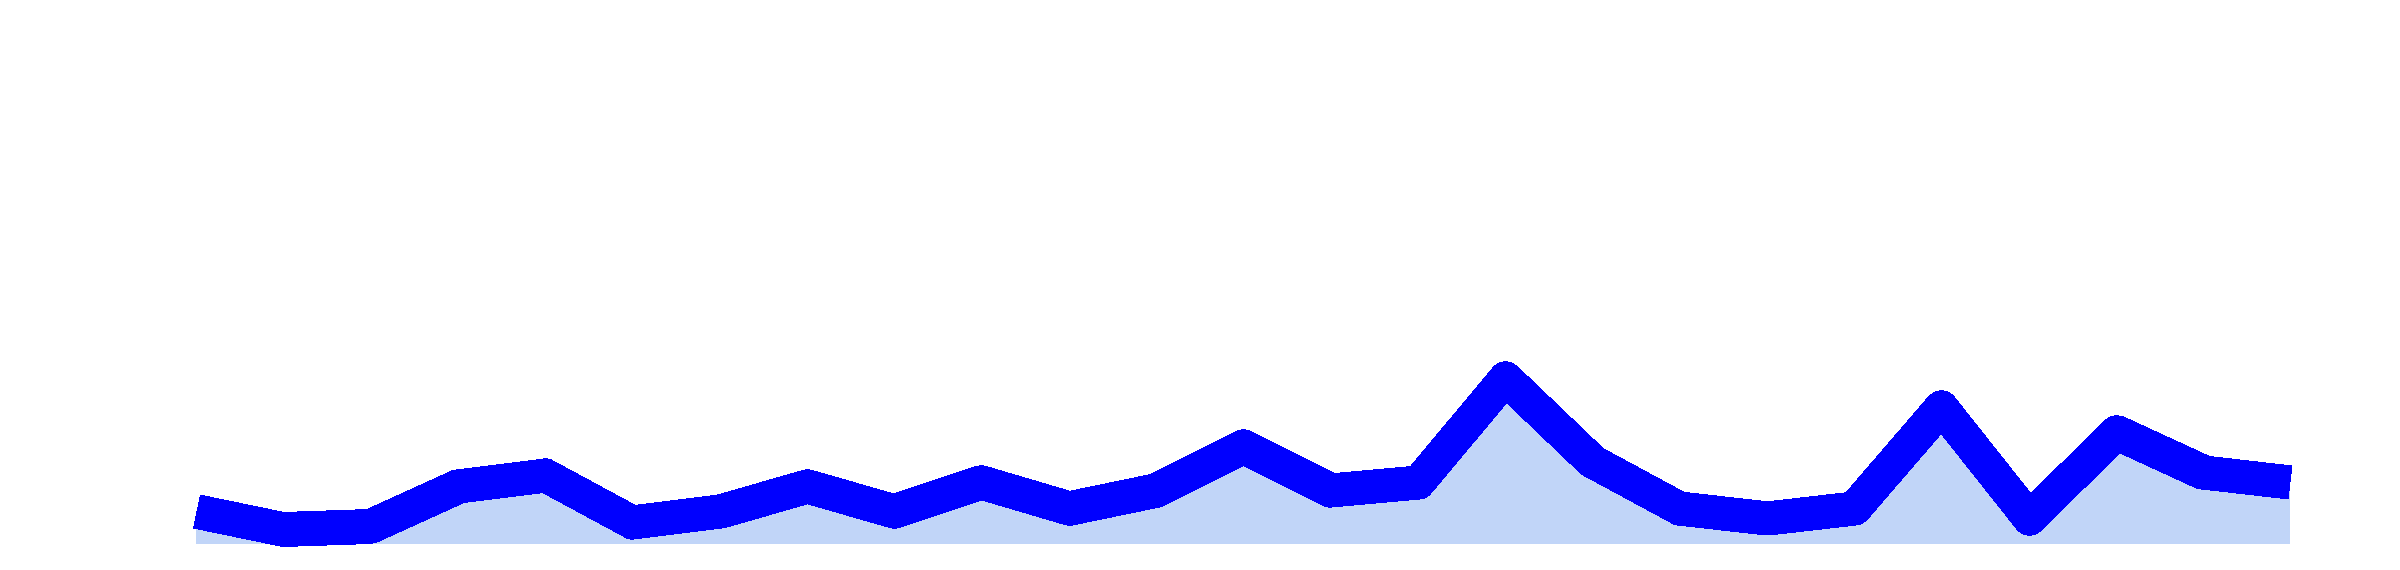
\includegraphics[width=2cm]{fig23.png}} & 1 & 0 & 120 & 121 & 596 & 47 & 47 & 47 & 47 & 47 & 47 & 0.45 & 586 & 607\\
24 & 807 & 400 & \raisebox{.12\height} {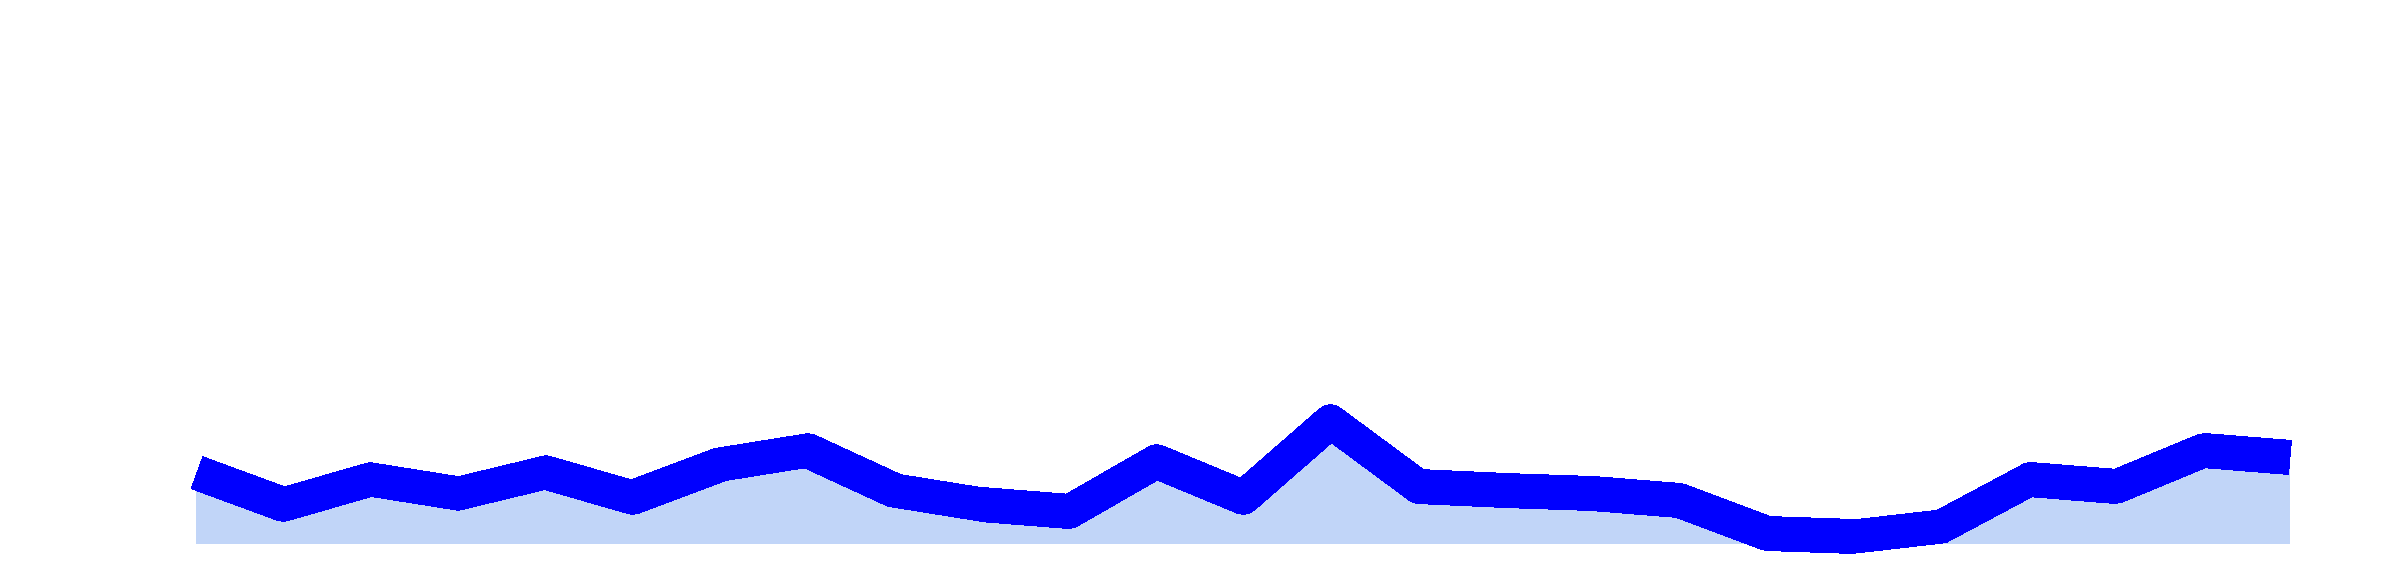
\includegraphics[width=2cm]{fig24.png}} & 0 & 0 & 131 & 131 & 566 & 48 & 48 & 48 & 47 & 48 & 48 & 0.73 & 571 & 616\\
25 & 1106 & 746 & \raisebox{.12\height} {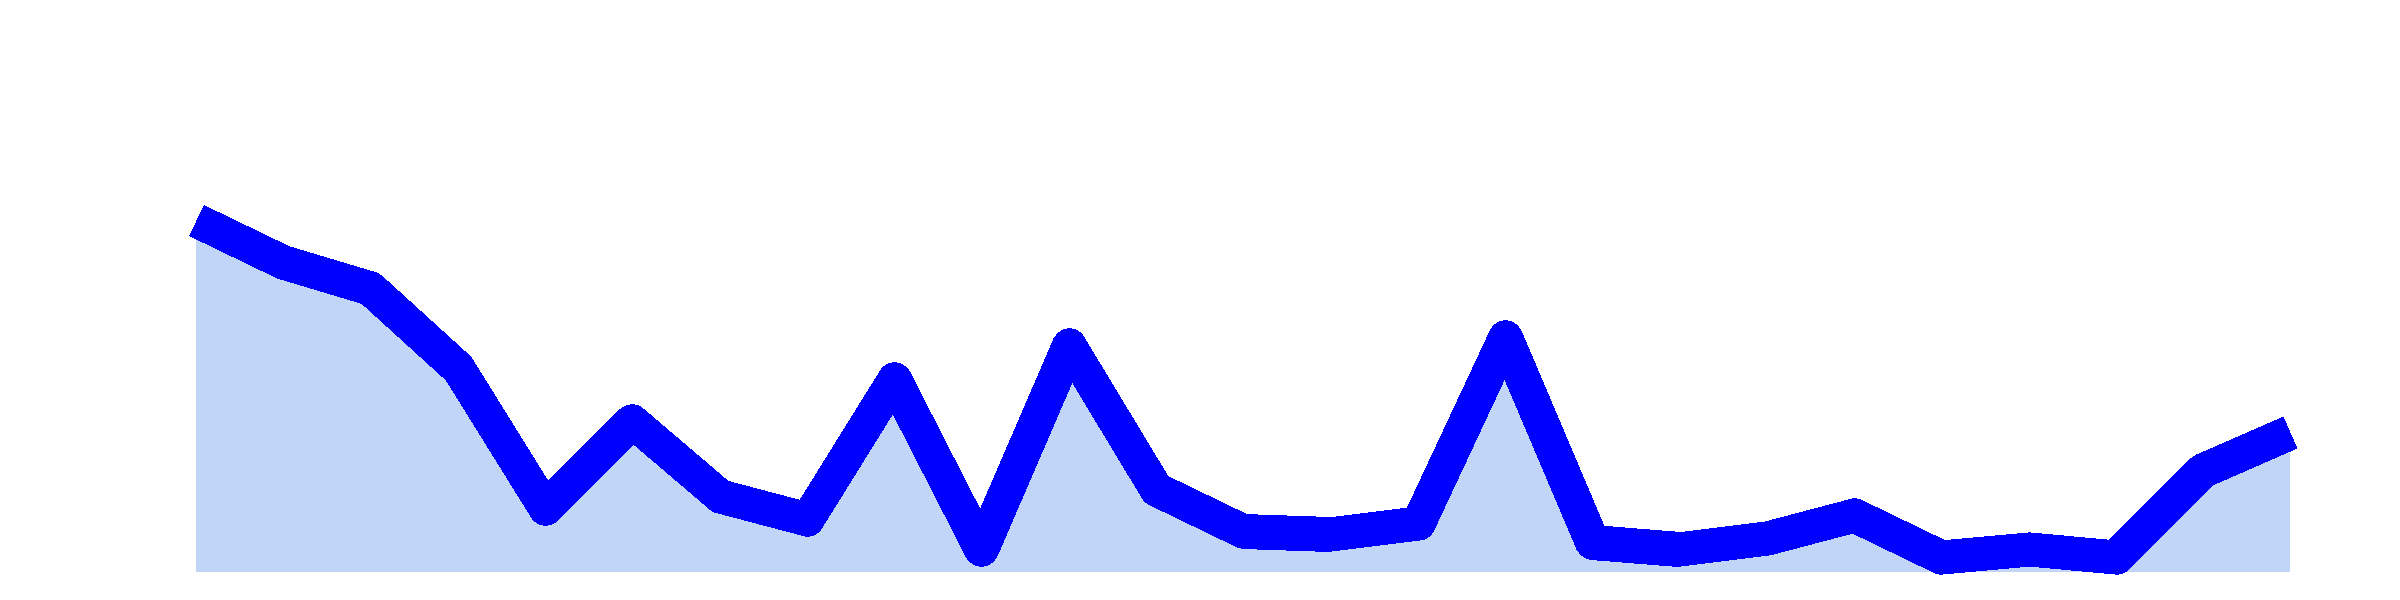
\includegraphics[width=2cm]{fig25.png}} & 1 & 0 & 112 & 113 & 522 & 58 & 58 & 58 & 57 & 58 & 58 & 0.67 & 503 & 548\\
26 & 561 & 252 & \raisebox{.12\height} {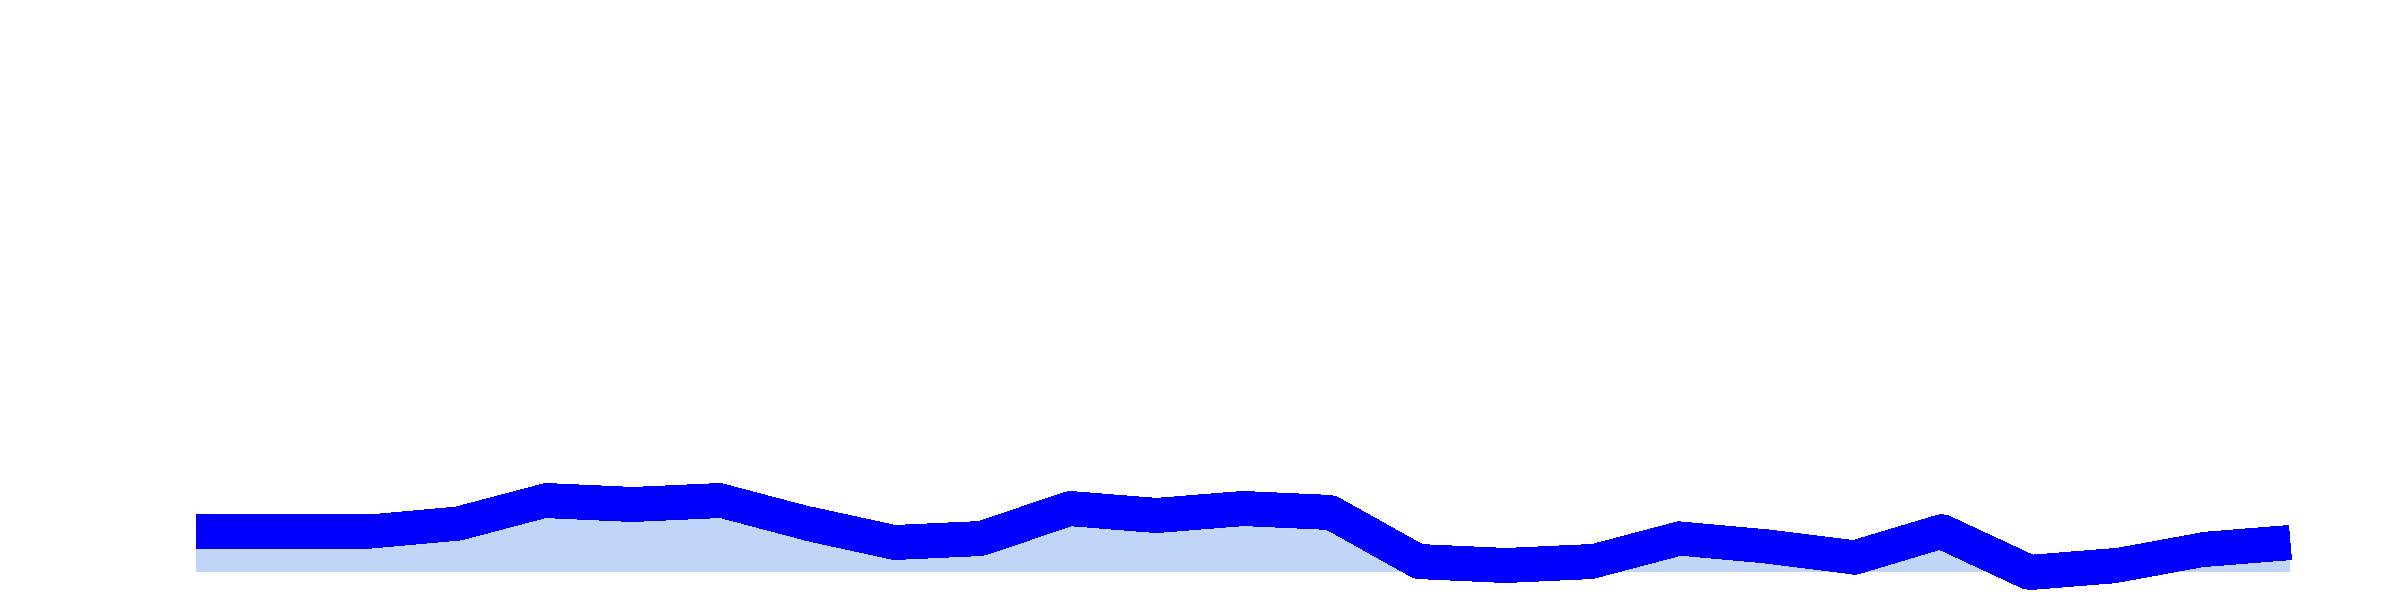
\includegraphics[width=2cm]{fig26.png}} & 1 & 0 & 84 & 85 & 578 & 53 & 52 & 52 & 52 & 52 & 53 & 0.58 & 552 & 641\\
27 & 938 & 463 & \raisebox{.12\height} {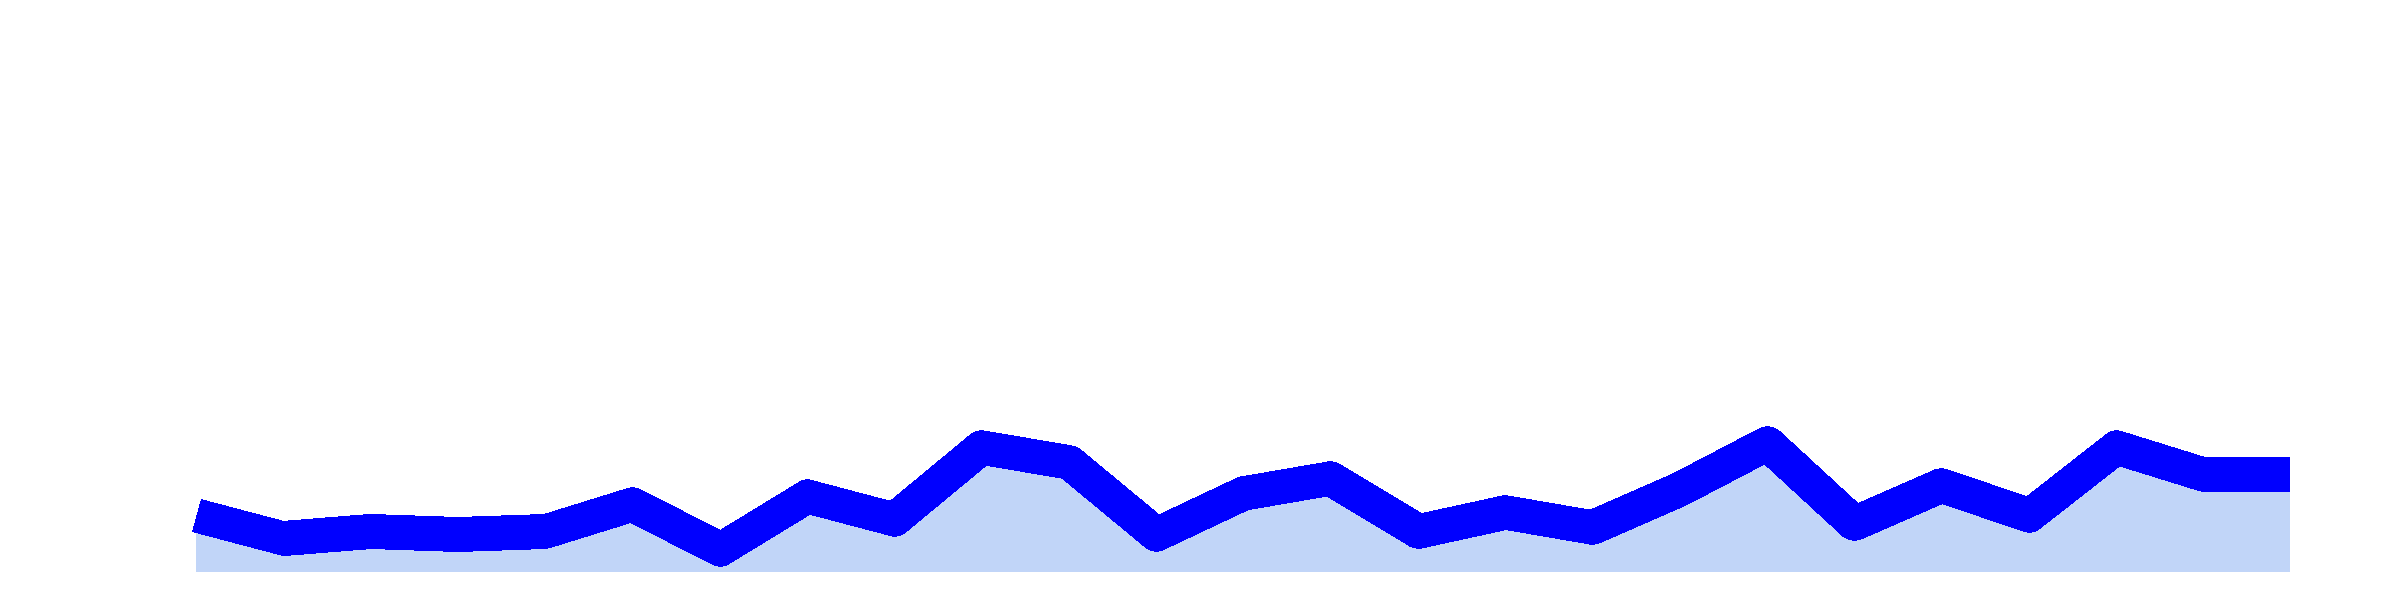
\includegraphics[width=2cm]{fig27.png}} & 2 & 0 & 135 & 137 & 583 & 40 & 40 & 40 & 40 & 40 & 40 & 0.73 & 536 & 588\\
28 & 1131 & 633 & \raisebox{.12\height} {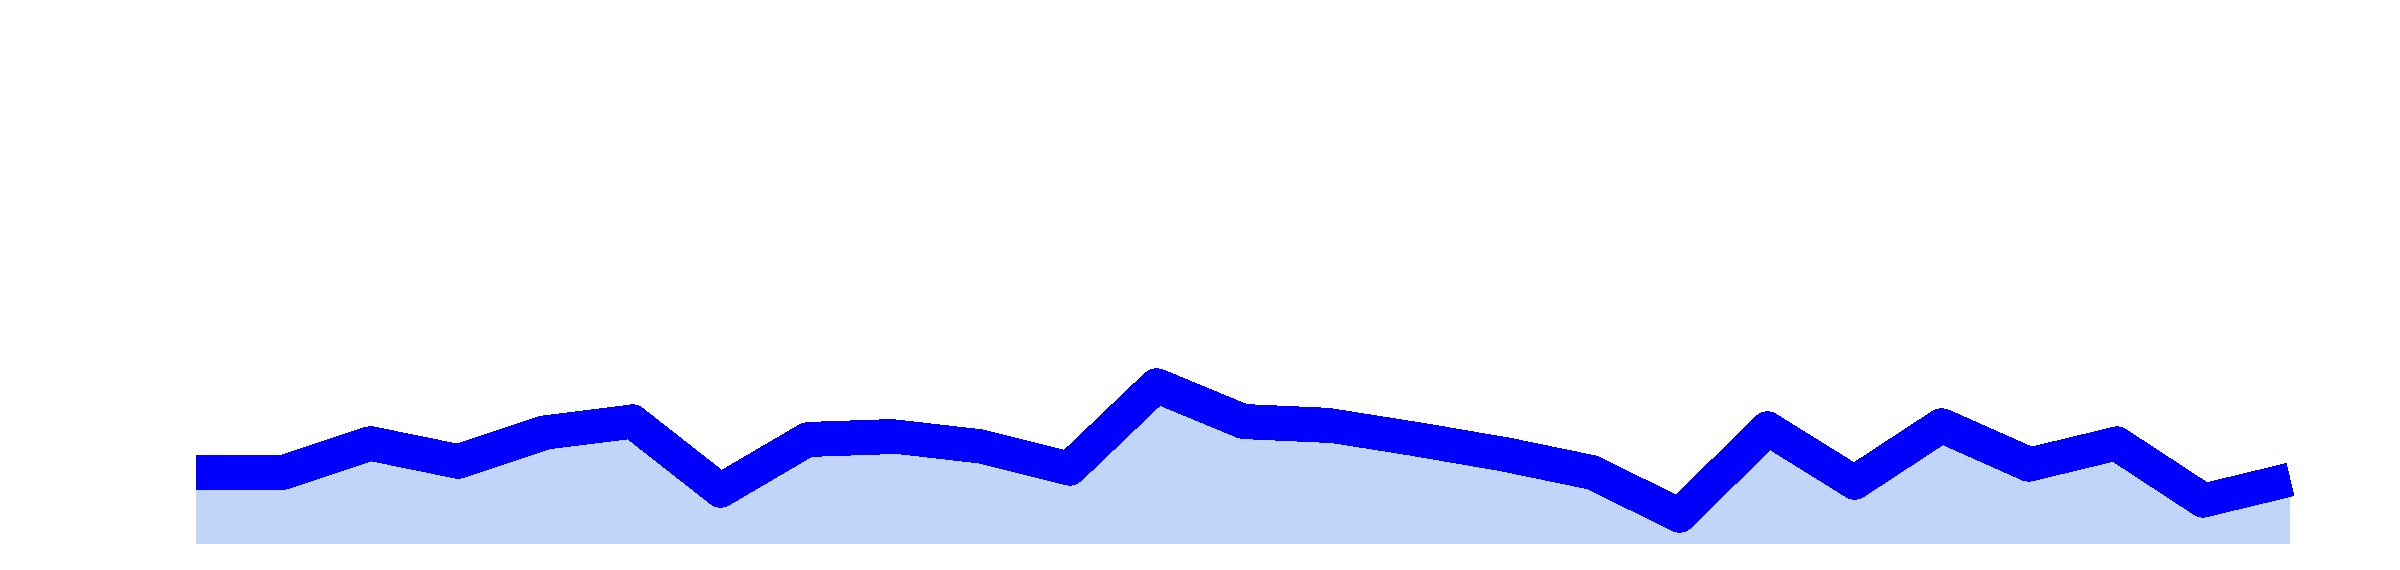
\includegraphics[width=2cm]{fig28.png}} & 0 & 0 & 135 & 135 & 548 & 45 & 45 & 45 & 45 & 45 & 45 & 0.60 & 531 & 580\\
29 & 1202 & 667 & \raisebox{.12\height} {\includegraphics[width=2cm]{fig29.png}} & 1 & 0 & 108 & 109 & 549 & 46 & 46 & 46 & 46 & 46 & 46 & 0.54 & 531 & 562\\
30 & 110 & 28 & \raisebox{.12\height} {\includegraphics[width=2cm]{fig30.png}} & 0 & 0 & 9 & 9 & 666 & 14 & 14 & 14 & 14 & 14 & 14 & 0.00 & 0 & 703\\
31 & 1183 & 476 & \raisebox{.12\height} {\includegraphics[width=2cm]{fig31.png}} & 2 & 0 & 125 & 127 & 605 & 52 & 52 & 52 & 52 & 52 & 52 & 0.58 & 588 & 665\\
32 & 664 & 244 & \raisebox{.12\height} {\includegraphics[width=2cm]{fig32.png}} & 1 & 0 & 64 & 65 & 619 & 55 & 55 & 55 & 55 & 55 & 55 & 0.33 & 594 & 637\\
33 & 243 & 92 & \raisebox{.12\height} {\includegraphics[width=2cm]{fig33.png}} & 1 & 0 & 22 & 23 & 612 & 19 & 19 & 19 & 19 & 19 & 19 & 0.53 & 544 & 642\\
34 & 2314 & 1033 & \raisebox{.12\height} {\includegraphics[width=2cm]{fig34.png}} & 0 & 0 & 147 & 147 & 588 & 51 & 46 & 46 & 46 & 46 & 51 & 0.17 & 584 & 613\\
35 & 738 & 297 & \raisebox{.12\height} {\includegraphics[width=2cm]{fig35.png}} & 0 & 0 & 100 & 100 & 615 & 52 & 50 & 50 & 49 & 50 & 52 & 0.08 & 569 & 610\\
36 & 1028 & 478 & \raisebox{.12\height} {\includegraphics[width=2cm]{fig36.png}} & 0 & 0 & 117 & 117 & 586 & 66 & 62 & 62 & 62 & 62 & 66 & 0.31 & 566 & 602\\
37 & 2092 & 928 & \raisebox{.12\height} {\includegraphics[width=2cm]{fig37.png}} & 0 & 0 & 115 & 115 & 594 & 47 & 47 & 47 & 47 & 47 & 47 & 0.30 & 576 & 617\\
38 & 308 & 84 & \raisebox{.12\height} {\includegraphics[width=2cm]{fig38.png}} & 0 & 0 & 33 & 33 & 677 & 26 & 26 & 26 & 26 & 26 & 26 & 0.19 & 571 & 733\\
39 & 20 & 9 & \raisebox{.12\height} {\includegraphics[width=2cm]{fig39.png}} & 0 & 0 & 1 & 1 & 537 & 6 & 6 & 6 & 6 & 6 & 6 & 0.17 & 602 & 635\\
40 & 9 & 3 & \raisebox{.12\height} {\includegraphics[width=2cm]{fig40.png}} & 0 & 0 & 1 & 1 & 641 & 1 & 0 & 0 & 0 & 0 & 1 & 0.00 & 0 & 0\\
41 & 539 & 152 & \raisebox{.12\height} {\includegraphics[width=2cm]{fig41.png}} & 0 & 0 & 56 & 56 & 667 & 53 & 53 & 53 & 53 & 53 & 53 & 0.45 & 638 & 701\\
42 & 1380 & 599 & \raisebox{.12\height} {\includegraphics[width=2cm]{fig42.png}} & 2 & 0 & 111 & 113 & 595 & 51 & 51 & 51 & 51 & 51 & 51 & 0.37 & 560 & 595\\
43 & 150 & 59 & \raisebox{.12\height} {\includegraphics[width=2cm]{fig43.png}} & 0 & 0 & 21 & 21 & 593 & 11 & 11 & 11 & 11 & 11 & 11 & 0.09 & 584 & 607\\
44 & 247 & 66 & \raisebox{.12\height} {\includegraphics[width=2cm]{fig44.png}} & 0 & 0 & 32 & 32 & 711 & 13 & 13 & 13 & 13 & 13 & 13 & 0.00 & 0 & 677\\
45 & 1208 & 646 & \raisebox{.12\height} {\includegraphics[width=2cm]{fig45.png}} & 3 & 0 & 139 & 142 & 567 & 51 & 51 & 51 & 51 & 51 & 51 & 0.86 & 545 & 564\\
46 & 1429 & 1031 & \raisebox{.12\height} {\includegraphics[width=2cm]{fig46.png}} & 2 & 0 & 119 & 121 & 512 & 49 & 49 & 49 & 49 & 49 & 49 & 0.63 & 513 & 579\\
47 & 1188 & 558 & \raisebox{.12\height} {\includegraphics[width=2cm]{fig47.png}} & 8 & 0 & 102 & 110 & 578 & 51 & 51 & 51 & 51 & 51 & 51 & 0.45 & 571 & 614\\
48 & 1102 & 557 & \raisebox{.12\height} {\includegraphics[width=2cm]{fig48.png}} & 0 & 0 & 114 & 114 & 570 & 52 & 52 & 52 & 52 & 52 & 57 & 0.46 & 552 & 591\\
49 & 1482 & 735 & \raisebox{.12\height} {\includegraphics[width=2cm]{fig49.png}} & 8 & 0 & 127 & 134 & 580 & 46 & 46 & 46 & 46 & 46 & 47 & 0.59 & 551 & 597\\
50 & 32 & 12 & \raisebox{.12\height} {\includegraphics[width=2cm]{fig50.png}} & 0 & 0 & 3 & 3 & 559 & 4 & 4 & 4 & 4 & 4 & 4 & 0.00 & 0 & 592\\
51 & 1350 & 674 & \raisebox{.12\height} {\includegraphics[width=2cm]{fig51.png}} & 1 & 0 & 122 & 123 & 563 & 58 & 58 & 58 & 58 & 58 & 63 & 0.59 & 549 & 565\\
52 & 39 & 13 & \raisebox{.12\height} {\includegraphics[width=2cm]{fig52.png}} & 0 & 0 & 1 & 1 & 573 & 10 & 10 & 10 & 10 & 10 & 10 & 0.40 & 674 & 643\\
53 & 1959 & 1128 & \raisebox{.12\height} {\includegraphics[width=2cm]{fig53.png}} & 0 & 0 & 139 & 139 & 548 & 56 & 56 & 56 & 56 & 56 & 56 & 0.45 & 525 & 558\\
54 & 2038 & 1233 & \raisebox{.12\height} {\includegraphics[width=2cm]{fig54.png}} & 0 & 0 & 119 & 119 & 559 & 67 & 47 & 47 & 44 & 47 & 67 & 0.49 & 519 & 567\\
55 & 1382 & 490 & \raisebox{.12\height} {\includegraphics[width=2cm]{fig55.png}} & 1 & 0 & 128 & 129 & 625 & 55 & 55 & 55 & 48 & 55 & 55 & 0.20 & 583 & 635\\
56 & 51 & 17 & \raisebox{.12\height} {\includegraphics[width=2cm]{fig56.png}} & 0 & 0 & 7 & 7 & 661 & 7 & 7 & 7 & 6 & 7 & 7 & 0.00 & 0 & 641\\
57 & 27 & 7 & \raisebox{.12\height} {\includegraphics[width=2cm]{fig57.png}} & 0 & 0 & 2 & 2 & 719 & 1 & 1 & 1 & 1 & 1 & 1 & 0.00 & 0 & 657\\
58 & 2123 & 1237 & \raisebox{.12\height} {\includegraphics[width=2cm]{fig58.png}} & 1 & 0 & 122 & 123 & 565 & 53 & 53 & 53 & 53 & 53 & 53 & 0.45 & 506 & 552\\
59 & 18 & 6 & \raisebox{.12\height} {\includegraphics[width=2cm]{fig59.png}} & 0 & 0 & 2 & 2 & 649 & 3 & 3 & 3 & 3 & 3 & 3 & 0.00 & 0 & 677\\
60 & 1370 & 840 & \raisebox{.12\height} {\includegraphics[width=2cm]{fig60.png}} & 1 & 0 & 151 & 152 & 543 & 49 & 49 & 49 & 49 & 49 & 49 & 0.55 & 546 & 571\\
61 & 264 & 120 & \raisebox{.12\height} {\includegraphics[width=2cm]{fig61.png}} & 2 & 0 & 28 & 30 & 575 & 44 & 44 & 44 & 44 & 44 & 44 & 0.45 & 558 & 648\\
62 & 184 & 87 & \raisebox{.12\height} {\includegraphics[width=2cm]{fig62.png}} & 0 & 0 & 27 & 27 & 590 & 29 & 29 & 29 & 29 & 29 & 29 & 0.79 & 563 & 595\\
63 & 323 & 113 & \raisebox{.12\height} {\includegraphics[width=2cm]{fig63.png}} & 0 & 0 & 56 & 56 & 641 & 35 & 35 & 35 & 35 & 35 & 35 & 0.29 & 612 & 658\\
64 & 64 & 24 & \raisebox{.12\height} {\includegraphics[width=2cm]{fig64.png}} & 0 & 0 & 10 & 10 & 647 & 6 & 6 & 6 & 6 & 6 & 6 & 0.17 & 652 & 641\\
65 & 1972 & 1100 & \raisebox{.12\height} {\includegraphics[width=2cm]{fig65.png}} & 2 & 1 & 140 & 143 & 552 & 60 & 60 & 60 & 60 & 60 & 61 & 0.47 & 523 & 566\\
66 & 773 & 459 & \raisebox{.12\height} {\includegraphics[width=2cm]{fig66.png}} & 0 & 0 & 139 & 139 & 543 & 44 & 44 & 44 & 44 & 44 & 44 & 0.64 & 547 & 577\\
67 & 1369 & 721 & \raisebox{.12\height} {\includegraphics[width=2cm]{fig67.png}} & 1 & 0 & 138 & 139 & 561 & 44 & 44 & 44 & 44 & 44 & 45 & 0.66 & 530 & 594\\
68 & 1173 & 654 & \raisebox{.12\height} {\includegraphics[width=2cm]{fig68.png}} & 1 & 0 & 134 & 135 & 559 & 52 & 52 & 52 & 52 & 52 & 52 & 0.33 & 532 & 568\\
69 & 1214 & 635 & \raisebox{.12\height} {\includegraphics[width=2cm]{fig69.png}} & 2 & 0 & 142 & 144 & 553 & 52 & 52 & 52 & 52 & 52 & 53 & 0.63 & 536 & 603\\
70 & 933 & 556 & \raisebox{.12\height} {\includegraphics[width=2cm]{fig70.png}} & 3 & 0 & 132 & 135 & 539 & 46 & 46 & 46 & 46 & 46 & 46 & 0.70 & 524 & 556\\
71 & 1388 & 695 & \raisebox{.12\height} {\includegraphics[width=2cm]{fig71.png}} & 0 & 0 & 110 & 110 & 557 & 49 & 49 & 49 & 49 & 49 & 49 & 0.57 & 526 & 570\\
72 & 1917 & 1111 & \raisebox{.12\height} {\includegraphics[width=2cm]{fig72.png}} & 1 & 0 & 130 & 131 & 551 & 61 & 61 & 61 & 61 & 61 & 61 & 0.48 & 552 & 558\\
73 & 773 & 398 & \raisebox{.12\height} {\includegraphics[width=2cm]{fig73.png}} & 9 & 0 & 109 & 118 & 576 & 53 & 53 & 53 & 53 & 53 & 53 & 0.62 & 558 & 592\\
74 & 1797 & 1035 & \raisebox{.12\height} {\includegraphics[width=2cm]{fig74.png}} & 0 & 0 & 118 & 118 & 570 & 46 & 46 & 46 & 46 & 46 & 46 & 0.54 & 542 & 610\\
75 & 67 & 25 & \raisebox{.12\height} {\includegraphics[width=2cm]{fig75.png}} & 0 & 0 & 7 & 7 & 626 & 11 & 11 & 11 & 11 & 11 & 11 & 0.36 & 548 & 631\\
76 & 24 & 9 & \raisebox{.12\height} {\includegraphics[width=2cm]{fig76.png}} & 0 & 0 & 4 & 4 & 645 & 4 & 2 & 2 & 2 & 2 & 4 & 0.50 & 530 & 625\\
77 & 1246 & 506 & \raisebox{.12\height} {\includegraphics[width=2cm]{fig77.png}} & 0 & 0 & 152 & 152 & 600 & 54 & 54 & 54 & 54 & 54 & 54 & 0.19 & 564 & 631\\
78 & 278 & 86 & \raisebox{.12\height} {\includegraphics[width=2cm]{fig78.png}} & 0 & 0 & 17 & 17 & 641 & 37 & 37 & 37 & 37 & 37 & 37 & 0.08 & 624 & 655\\
79 & 283 & 106 & \raisebox{.12\height} {\includegraphics[width=2cm]{fig79.png}} & 0 & 0 & 32 & 32 & 606 & 29 & 29 & 29 & 29 & 29 & 29 & 0.14 & 665 & 611\\
80 & 848 & 347 & \raisebox{.12\height} {\includegraphics[width=2cm]{fig80.png}} & 0 & 0 & 127 & 127 & 623 & 52 & 52 & 52 & 52 & 52 & 52 & 0.73 & 619 & 643\\
81 & 75 & 15 & \raisebox{.12\height} {\includegraphics[width=2cm]{fig81.png}} & 0 & 0 & 2 & 2 & 754 & 10 & 10 & 10 & 10 & 10 & 10 & 0.20 & 697 & 806\\
82 & 1667 & 924 & \raisebox{.12\height} {\includegraphics[width=2cm]{fig82.png}} & 0 & 0 & 126 & 126 & 543 & 50 & 50 & 50 & 50 & 50 & 50 & 0.58 & 561 & 592\\
83 & 776 & 281 & \raisebox{.12\height} {\includegraphics[width=2cm]{fig83.png}} & 0 & 0 & 71 & 71 & 621 & 46 & 46 & 46 & 46 & 46 & 46 & 0.26 & 593 & 650\\
84 & 1320 & 623 & \raisebox{.12\height} {\includegraphics[width=2cm]{fig84.png}} & 3 & 0 & 140 & 143 & 589 & 47 & 47 & 47 & 47 & 47 & 47 & 0.49 & 565 & 612\\
85 & 1415 & 648 & \raisebox{.12\height} {\includegraphics[width=2cm]{fig85.png}} & 0 & 0 & 137 & 137 & 579 & 49 & 49 & 49 & 49 & 49 & 49 & 0.39 & 570 & 591\\
86 & 1381 & 681 & \raisebox{.12\height} {\includegraphics[width=2cm]{fig86.png}} & 0 & 0 & 127 & 127 & 573 & 51 & 51 & 51 & 51 & 50 & 51 & 0.24 & 572 & 577\\
87 & 635 & 244 & \raisebox{.12\height} {\includegraphics[width=2cm]{fig87.png}} & 0 & 0 & 97 & 97 & 612 & 47 & 47 & 47 & 47 & 47 & 47 & 0.43 & 597 & 619\\
\midrule
\textbf{Total} & \textbf{92167} & \textbf{48092} & \textbf{\raisebox{.12\height} {\includegraphics[width=2cm]{figTotal.png}}} & \textbf{77} & \textbf{1} & \textbf{8200} & \textbf{8274} & \textbf{} & \textbf{3669} & \textbf{3603} & \textbf{3604} & \textbf{3587} & \textbf{3602} & \textbf{3691} & \textbf{} & \textbf{} & \textbf{}\\*
\end{longtable}
\endgroup{}
\end{landscape}
\clearpage

\section{SUMMARY OF BIOLOGICAL DATA FOR ROUGHEYE/BLACKSPOTTED ROCKFISH COMPLEX.}
\label{app:sixth-appendix}

Biological data collected for rougheye/blackspotted rockfish complex. Each set is listed with counts of specimens sampled, calculations of mean fork lengths and number of species visually identified as either a RE = rougheye rockfish, BS = blackspotted rockfish or a hybrid. ~\\
\hspace*{0.333em}\\
\begin{landscape}\begingroup\fontsize{8}{10}\selectfont
\begin{longtable}{>{\raggedright\arraybackslash}p{3.5cm}>{\raggedleft\arraybackslash}p{0.7cm}>{\centering\arraybackslash}p{0.7cm}>{\centering\arraybackslash}p{0.7cm}>{\centering\arraybackslash}p{0.7cm}>{\centering\arraybackslash}p{0.7cm}>{\centering\arraybackslash}p{0.7cm}>{\centering\arraybackslash}p{0.7cm}>{\centering\arraybackslash}p{0.7cm}>{\centering\arraybackslash}p{1.1cm}>{\centering\arraybackslash}p{0.7cm}>{\centering\arraybackslash}p{0.7cm}>{\centering\arraybackslash}p{0.7cm}>{\centering\arraybackslash}p{1.0cm}>{\centering\arraybackslash}p{1.2cm}>{\centering\arraybackslash}p{0.8cm}}
\toprule
\multicolumn{2}{c}{\textbf{ }} & \multicolumn{7}{c}{\textbf{Specimen Count}} & \multicolumn{4}{c}{\textbf{Mean Fork Length(mm)}} & \multicolumn{3}{c}{\textbf{Sampler Visual id Count}} \\
\cmidrule(l{3pt}r{3pt}){3-9} \cmidrule(l{3pt}r{3pt}){10-13} \cmidrule(l{3pt}r{3pt}){14-16}
\textbf{Species Name} & \textbf{Set} & \textbf{Fork Length} & \textbf{Weight} & \textbf{Sex} & \textbf{Maturity} & \textbf{Otolith} & \textbf{DNA} & \textbf{Total Count} & \textbf{Proportion Males} & \textbf{Males} & \textbf{Females} & \textbf{No sex} & \textbf{RE} & \textbf{BS} & \textbf{Hybrid}\\
\midrule
\endfirsthead
\multicolumn{16}{@{}l}{continued.}\\
\toprule
\multicolumn{2}{c}{\textbf{ }} & \multicolumn{7}{c}{\textbf{Specimen Count}} & \multicolumn{4}{c}{\textbf{Mean Fork Length(mm)}} & \multicolumn{3}{c}{\textbf{Sampler Visual id Count}} \\
\cmidrule(l{3pt}r{3pt}){3-9} \cmidrule(l{3pt}r{3pt}){10-13} \cmidrule(l{3pt}r{3pt}){14-16}
\textbf{Species Name} & \textbf{Set} & \textbf{Fork Length} & \textbf{Weight} & \textbf{Sex} & \textbf{Maturity} & \textbf{Otolith} & \textbf{DNA} & \textbf{Total Count} & \textbf{Proportion Males} & \textbf{Males} & \textbf{Females} & \textbf{No sex} & \textbf{RE} & \textbf{BS} & \textbf{Hybrid}\\
\midrule
\endhead

\endfoot
\bottomrule
\endlastfoot
ROUGHEYE/ BLACKSPOTTED ROCKFISH COMPLEX & 5 & 2 & 2 & 2 & 2 & 2 & 2 & 2 & 0.5 & 481 & 526 & 0 & 2 & 0 & 0\\
 & 14 & 7 & 7 & 7 & 7 & 7 & 7 & 7 & 0.57 & 457 & 494 & 0 & 5 & 2 & 0\\
 & 20 & 11 & 11 & 11 & 11 & 11 & 11 & 11 & 0.55 & 484 & 487 & 0 & 8 & 3 & 0\\
 & 23 & 4 & 4 & 4 & 4 & 4 & 4 & 4 & 0.5 & 468 & 483 & 0 & 2 & 2 & 0\\
 & 31 & 1 & 1 & 1 & 1 & 1 & 1 & 1 & 0 & 0 & 516 & 0 & 1 & 0 & 0\\
 & 34 & 1 & 1 & 1 & 1 & 1 & 1 & 1 & 1 & 389 & 0 & 0 & 1 & 0 & 0\\
 & 37 & 3 & 3 & 3 & 3 & 3 & 3 & 3 & 0.67 & 485 & 525 & 0 & 3 & 0 & 0\\
 & 42 & 1 & 1 & 1 & 1 & 1 & 1 & 1 & 0 & 0 & 450 & 0 & 0 & 1 & 0\\
 & 50 & 1 & 1 & 1 & 1 & 1 & 1 & 1 & 0 & 0 & 667 & 0 & 1 & 0 & 0\\
 & 55 & 18 & 18 & 18 & 18 & 18 & 18 & 18 & 0.61 & 450 & 438 & 0 & 4 & 14 & 0\\
 & 65 & 1 & 1 & 1 & 1 & 1 & 1 & 1 & 1 & 533 & 0 & 0 & 0 & 1 & 0\\
 & 69 & 3 & 3 & 3 & 3 & 3 & 3 & 3 & 0.67 & 518 & 546 & 0 & 1 & 2 & 0\\
 & 71 & 25 & 25 & 25 & 25 & 25 & 25 & 25 & 0.44 & 498 & 498 & 0 & 9 & 16 & 0\\
 & 72 & 3 & 3 & 3 & 3 & 3 & 3 & 3 & 0.33 & 490 & 483 & 0 & 1 & 2 & 0\\
 & 77 & 2 & 2 & 2 & 2 & 2 & 2 & 2 & 0.5 & 581 & 574 & 0 & 1 & 1 & 0\\
 & 83 & 22 & 22 & 22 & 22 & 22 & 22 & 22 & 0.5 & 464 & 471 & 0 & 14 & 8 & 0\\
 & 84 & 2 & 2 & 2 & 2 & 2 & 2 & 2 & 1 & 470 & 0 & 0 & 2 & 0 & 0\\
 & 85 & 11 & 11 & 10 & 10 & 11 & 11 & 11 & 0.5 & 458 & 477 & 408 & 8 & 3 & 0\\
 & 86 & 2 & 2 & 2 & 2 & 2 & 2 & 2 & 0.5 & 495 & 459 & 0 & 2 & 0 & 0\\
 & 87 & 6 & 6 & 6 & 6 & 6 & 6 & 6 & 0.67 & 486 & 492 & 0 & 3 & 3 & 0\\
\midrule
\textbf{Total} & \textbf{} & \textbf{126} & \textbf{126} & \textbf{125} & \textbf{125} & \textbf{126} & \textbf{126} & \textbf{126} & \textbf{} & \textbf{} & \textbf{} & \textbf{} & \textbf{68} & \textbf{58} & \textbf{0}\\*
\end{longtable}
\endgroup{}
\end{landscape}
\clearpage

\end{appendices}

\clearpage

\hypertarget{references}{%
\section{References}\label{references}}

\noindent \vspace{-2em} \setlength{\parindent}{-0.2in} \setlength{\leftskip}{0.2in} \setlength{\parskip}{8pt}

\hypertarget{refs}{}
\leavevmode\hypertarget{ref-Amaya2020}{}%
Amaya, M., D. J. 2020. Physical drivers of the summer 2019 North Pacific marine heatwave. Nat Commun (11, 1903).

\leavevmode\hypertarget{ref-Bond2015}{}%
Bond, N.A., Cronin, M.F., Freeland, H., and Mantua, N. 2015. Causes and impacts of the 2014 warm anomaly in the NE Pacific. Geophysical Research Letters 42(9): 3414--3420.

\leavevmode\hypertarget{ref-DFO2020}{}%
DFO. 2020. Evaluating the robustness of candidate management procedures in the BC Sablefish (\emph{Anoplopoma fimbria}) fishery for 2019-2020. DFO Can. Sci. Advis. Sec. Sci. Resp. (25).

\leavevmode\hypertarget{ref-DORANTESGILARD2020}{}%
Dorantes-Gilardi, M., and Rivas, D. 2019. Effects of the 2013-2016 Northeast Pacific warm anomaly on physical and biogeochemical variables off northwestern Baja California, derived from a numerical NPZD ocean model. Deep Sea Research Part II: Topical Studies in Oceanography 169-170: 104668.

\leavevmode\hypertarget{ref-Downes1997}{}%
Downes, A.J., Andrews, W.T., Smith, M.S., Saunders, M.W., and Jewsbury., G.D. 1997. Cruise details of Sablefish (\emph{Anoplopoma fimbria}) surveys conducted in B.C. waters, 1994-1995. Can. Data Rep. Fish. Aquat. Sci. 1997/1007: 106 p.

\leavevmode\hypertarget{ref-Lacko2020}{}%
Lacko, L.C., Acheson, S.M., and Connors, B.M. 2020. Summary of the annual 2018 and 2019 sablefish (\emph{Anoplopoma fimbria}) trap surveys, October 9 - November 19, 2018 and October 8 - November 25, 2019. Can. Data Rep. Fish. Aquat. Sci. 2020/3396: vii + 66 p.

\leavevmode\hypertarget{ref-Olsen2010}{}%
Olsen, N. 2010. CA user's guide to GFBioField: The Pacific Region's at-sea data acquisition system for groundfish trawl surveys. Can. Tech. Rep. Fish.Aquat. Sci. 2010/2887: x + 76 p.

\leavevmode\hypertarget{ref-Orr2008}{}%
Orr, J., and Wildes, S. 2008. Species of the rougheye rockfish complex: Resurrection of Sebastes melanostictus (Matsubara, 1934) and a redescription of Sebastes aleutianus (Jordan and Evermann, 1898) (Teleostei: Scorpaeniformes). Fishery Bulletin- National Oceanic and Atmospheric Administration 106: 111--134.

\leavevmode\hypertarget{ref-Smith1996}{}%
Smith, M.S., Saunders, M.W., and Andrews, W.T. 1996. Cruise details of sablefish (\emph{Anoplopoma fimbria}) surveys conducted in B.C. waters 1988-1993. Can. Tech. Rep. Fish.Aquat. Sci. 1996/976: 129 p.

\leavevmode\hypertarget{ref-Wyeth2003}{}%
Wyeth, M.R., and Kronlund, A.R. 2003. Sablefish (\emph{Anoplopoma fimbria}) Research and Assessment Surveys conducted in British Columbia waters from 1996 through 2000. Can. Data Rep. Fish. Aquat. Sci. 2003/1116: 130 p.

\leavevmode\hypertarget{ref-Wyeth2004b}{}%
Wyeth, M.R., Kronlund, A.R., and Elfert, M. 2004a. Summary of the 2003 British Columbia Sablefish (\emph{Anoplopoma fimbria}) Research and Assessment Survey. Can. Data Rep. Fish. Aquat. Sci. 2004/1148: 68 p.

\leavevmode\hypertarget{ref-Wyeth2004a}{}%
Wyeth, M.R., Kronlund, A.R., and Elfert, M. 2004b. Summary of the 2002 British Columbia Sablefish (\emph{Anoplopoma fimbria}) Research and Assessment Survey. Can. Data Rep. Fish. Aquat. Sci. 2004/1140: 59 p.

\leavevmode\hypertarget{ref-Wyeth2006}{}%
Wyeth, M.R., Kronlund, A.R., and Elfert, M. 2006. Summary of the 2004 British Columbia Sablefish (\emph{Anoplopoma fimbria}) Research and Assessment Surveys. Can. Data Rep. Fish. Aquat. Sci. 2006/2660: 74 p.
\end{document}
